\documentclass[a4paper]{article}

% Setup pdf creation
\usepackage[pdftex,bookmarks=true,pdfpagemode=UseOutlines,pdfborder={0 0 0},bookmarksopen=true]{hyperref}
\hypersetup{pdftitle={Master Thesis, Ulf Aslak}}

% Everything Non-content is put in style.sty
\usepackage{style}

% Uncomment and fill in if you want default front page
% \title{Personality archetypes reveal evolutionarily important behavioral strategies} 
% \author{Ulf Aslak}


\begin{document}


% Frontpage (custom)
% ------------------
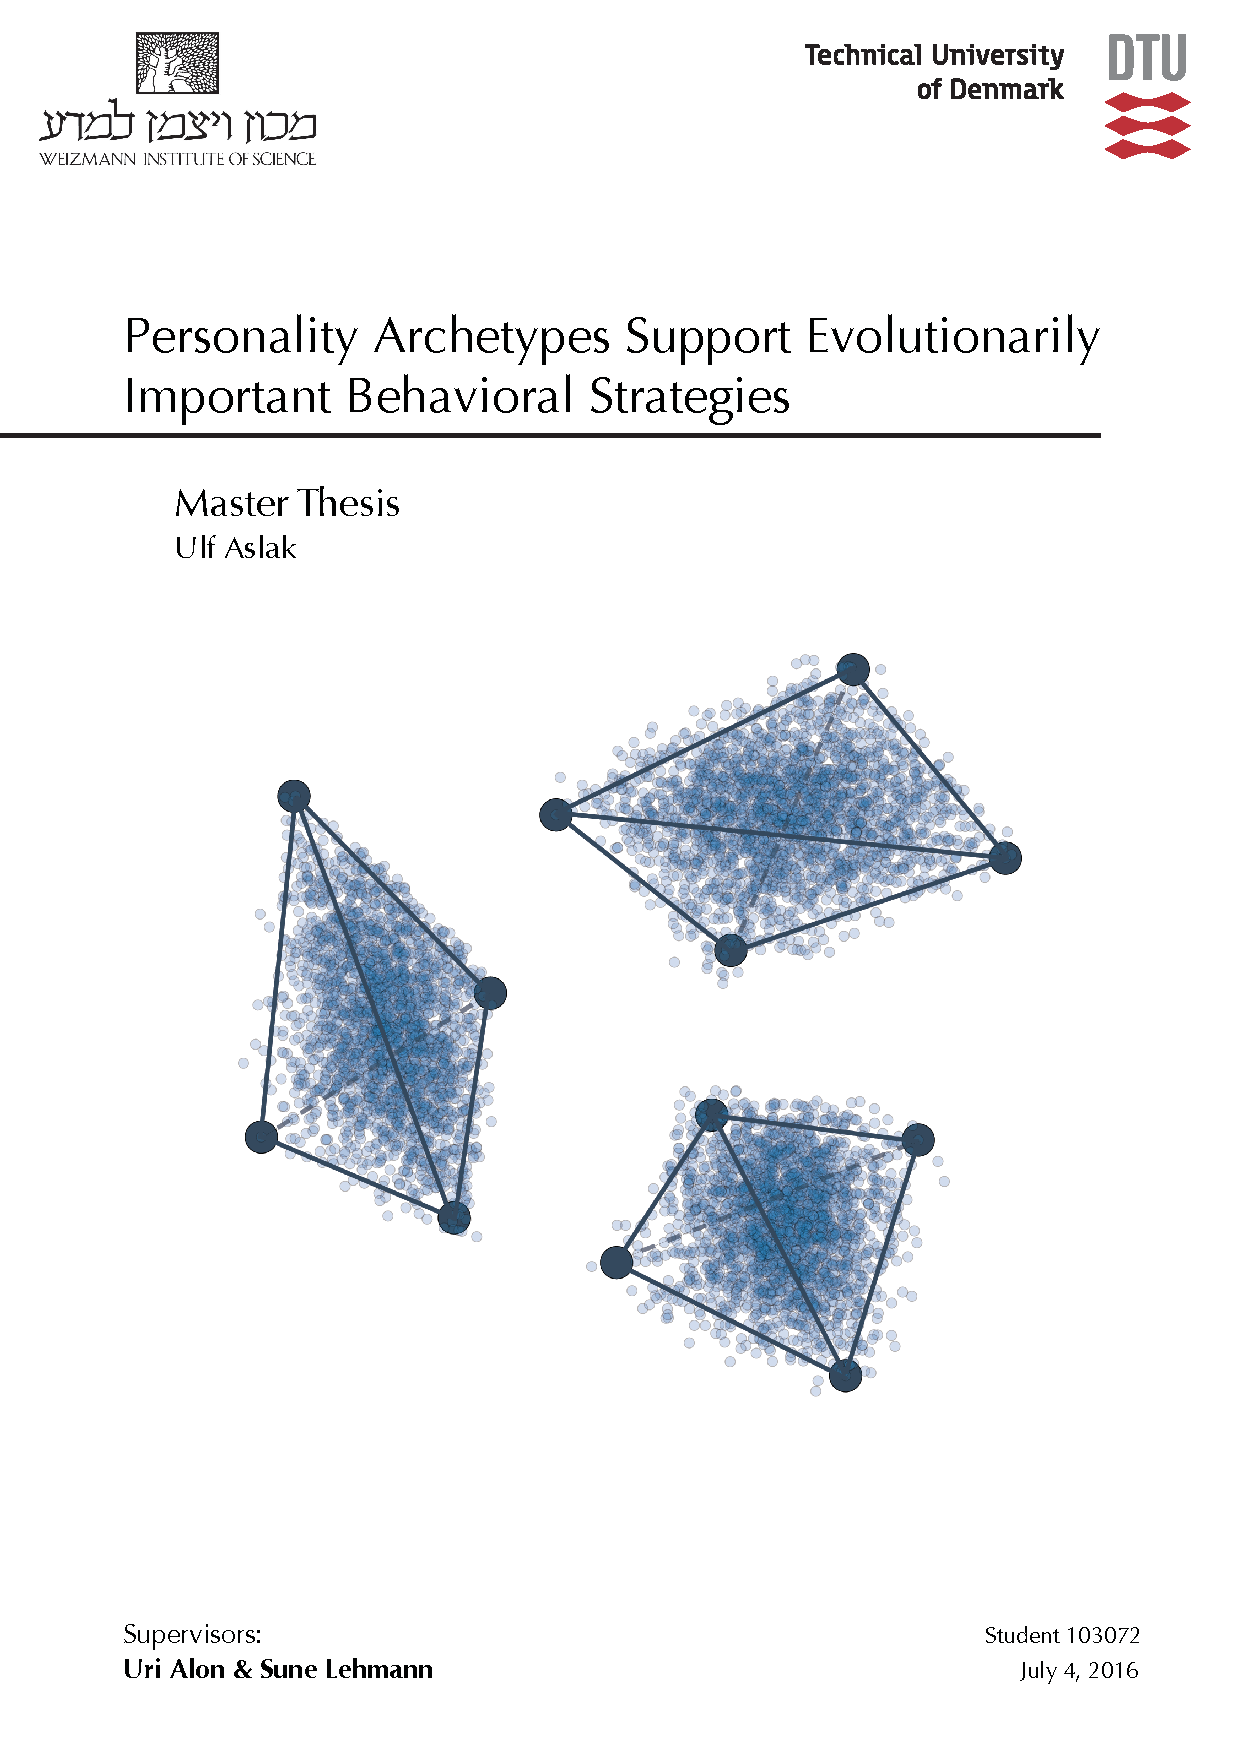
\includepdf{figures/frontpage}


% % Frontpage (default)
% ------------------
% \maketitle 
% \mbox{}
% \thispagestyle{empty}
% \newpage


% Preface
% -------
\pagenumbering{roman}
\section*{Preface}
\addcontentsline{toc}{section}{Preface}
This thesis was submitted as a final requirement for obtaining the degree of Master of Digital Media Engineering (cand. polyt.) at the Technical University of Denmark (DTU). It was carried out from january to july of 2016 as a collaboration between the Uri Alon Lab, at the Weizmann Institute of Science (WIS) in Israel, and the Social Fabric project at University of Copenhagen and DTU Compute. Throughout the project I lived in Israel and appeared in the lab where I, aside from conducting my own research, participated in group meetings, project sparing, and various other research activities. The project was mainly supervised by Uri Alon (Professor, WIS, Dept. of Molecular Cell Biology) and Sune Lehmann (Associate Professor, DTU, DTU Compute). Hila Sheftel and Pablo Szekely (PhD students, WIS, Dept. of Molecular Cell Biology) also took part in supervising and mentoring. 

I want to thank Uri for actively engaging in my work with childlike curiosity and genuine interest, and for never failing to identify the paths to the most interesting research objectives. I thank Sune for always believing in me and my motivations, for facilitating the whole arrangement and for his infinite resource of spirit. I thank Hila and Pablo for invaluable scientific guidance and mentoring, Avi Mayo for technical discussions of various sorts, all the members of the Theatre Lab for inspiration and enlightenment, and everyone in the Uri Alon Lab for accepting me as a member of their nurturing research environment. I also thank my dear friend Daniel Svendsen for endless videocall discussions about the hardship of research and the meaning of life.

For economical support I want to thank Oticon Fonden, Reinholdt W. Jorck og Hustrus Fond, Ingeni\o rforeningen i Danmarks og Berg-Nielsens Studie- og St\o ttefond, KnuH\o jgaards Fond, Dansk Tennisfond, Otto M\o nsteds Fond and Dansk-Israelsk Studiefond.

Finally, I thank Vivi Lai for her tremendous courage and faith, and for letting me travel so far away for so long and still be right there, in the hammock by the window, upon my return.

\begin{figure}[!ht]
	\begin{minipage}[l]{\textwidth}
		\flushleft
		
\includegraphics[width=0.3\textwidth]{figures/underskrift}
	\end{minipage}
	\begin{minipage}[l]{\textwidth}
		\flushleft
		$\,\,\,$Ulf Aslak\\
		$\,\,\,$July 4th, 2016
	\end{minipage}
\end{figure}
\newpage


% Abstract
% --------
\section*{Abstract}
\addcontentsline{toc}{section}{Abstract}
Evolutionary psychology suggests that different strategies for performing evolutionarily important tasks shaped our personality differences. But what these strategies are remain guesswork. Here, we apply Pareto Task Inference to infer the strategies and their behavioral correlates. We find the same six personality archetypes to consistently emerge from archetypal analysis applied to a diverse selection of datasets describing personality of millions in broad western culture. Enrichment of demographic attributes, personality facets, values and behavior near the archetypes reveal behavioral strategies, some of which are mentioned in the literature. We test how well distance from personality archetypes can be predicted for individuals using behavioral data, and compare the resulting accuracy to that of prediction models for Big Five traits and Big Five questionnaire inventory principal components. We find that distance from personality archetypes can be predicted more accurately than the other personality targets. Based on the findings and supported by literature in evolutionary psychology we argue that personality archetypes can be viewed as fundamental behavioral strategies.
\newpage


% Resume
% ------
\section*{Resume}
\addcontentsline{toc}{section}{Resume}
Evolution\ae r psykologi foresl\aa r at forskellige strategier for at udf\o re evolution\ae rt vigtige opgaver i livet har formet vores individuelle forskelle som mennesker. Men hvad disse strategier er har indtil videre v\ae ret g\ae tv\ae rk. Her anvender vi Pareto Task Inference til at udlede strategierne og deres adf\ae rdsm\ae ssige korrelater. Vi finder, at de samme seks personlighedsarketyper opst\aa r, p\aa  konsistent vis, p\aa \, tv\ae rs af et diverst ensemble af datas\ae t, som til sammen beskriver personligheder af millioner af mennesker i den vestlige verden. Berigelse n\ae r arketyper af variable som demografiske attributter, personlighedsfacetter, menneskelige v\ae rdier og adf\ae rd m\aa lt gennem smartphones, giver evidens for forskellige personlighedsstrategier hvoraf nogle r\ae sonnerer med kendte strategier fra literaturen. Vi sammenligner hvor godt individuel afstand fra personlighedsarketyper, Big Five tr\ae k samt principiel-komponenter af varians i sp\o rgeskema-svar kan modelleres ud fra adf\ae rdsdata. Simuleringen viser at afstand fra personlighedsarketyper kan modelleres bedst. P\aa \, baggrund af disse resultater, og underst\o ttet af litteratur i evolution\ae r psykologi, foresl\aa r vi at de fundne personlighedsarketyper kan betragtes som fundamentale adf\ae rdsstrategier.

\newpage


% Table of contents
% -----------------
\begin{spacing}{1.22}
	\begin{adjustwidth}{-1cm}{-1cm}
		\setcounter{tocdepth}{4}
		\thispagestyle{plain}
		\renewcommand\contentsname{Table of Contents}
		\tableofcontents
		\newpage
	\end{adjustwidth}
\end{spacing}


% % Nomenclature
% % ------------
% \begin{spacing}{1.41}

% 	% Abbreviations
% 	\section*{List of Abbreviations}
% 	\addcontentsline{toc}{section}{List of Abbreviations}
% 	\thispagestyle{plain}
% 	\begin{longtable}{m{2.5cm} m{6.0cm} m{2.5cm}}
Abbreviation \& Acronyms \T \B & Interpretation \T \B & \T \B  \\

\hline 
DTU \T& \multicolumn{2}{l}{The Technical University of Denmark} \\
no. \T& \multicolumn{2}{l}{number of} \\
SD \T& \multicolumn{2}{l}{standard deviation} \\
NDA \T& \multicolumn{2}{l}{non-disclosure agreement} \\
AA \T& \multicolumn{2}{l}{archetypal analysis} \\
KDE \T& \multicolumn{2}{l}{Kernel Density Estimation} \\
BF \T& \multicolumn{2}{l}{Big Five} \\
BFM \T& \multicolumn{2}{l}{Big Five model} \\
FFM \T& \multicolumn{2}{l}{Five Factor model} \\
EP \T& \multicolumn{2}{l}{evolutionary psychology} \\
sig. \T& \multicolumn{2}{l}{significance} \\
PC \T& \multicolumn{2}{l}{principle component} \\
QI \T& \multicolumn{2}{l}{questionnaire item} \\
F2F \T& \multicolumn{2}{l}{face-to-face} \\

\\
\end{longtable}


% 	\newpage

% 	% Symbols
% 	\setcounter{secnumdepth}{0}
% 	\section{List of Symbols}
% 	\thispagestyle{plain}
% 	\begin{longtable}{m{1.5cm} m{7cm} m{2.5cm}}

% List of symbols
Symbol \T \B & Description \\
\hline

$d$ \T & Number of spacial components \\
$n$ \T & sample size \\
$\matr{A}$ \T & Archetype tensor \\


$\,$\\\\

% List of subscripts
Subscript & Description \\
\hline

$a$ \T & Archetype tensor archetype-index (0th axis) \\
$t$ \T & Archetype tensor trait-index (1st axis) \\
$D$ \T & Archetype tensor dataset-index (2nnd axis) \\

\end{longtable}


% 	\newpage

% 	% Glossary
% 	\setcounter{secnumdepth}{0}
% 	\section{Glossary}
% 	\thispagestyle{plain}
% 	\subparagraph*{Indicator} High-level unit of behavior measured in the data. Practically interchangable with what is commonly referred to as a \textit{feature} in statistics and machine learning, but is called indicator, because behavior is dynamic and can thus only be quantified as an indication, not a feature which linguistically is something more static.
\subparagraph*{Conversation} Set of interactions (\texttt{text}, \texttt{call}, \texttt{F2F}) grouped by max. time distance criteria. For \texttt{text} this forms intuitive text conversations, and similarly for \texttt{call} it corresponds to missed calls returned a short time after but could potentially be an indefinite series of back and forth calls. For \texttt{F2F} a \textit{conversation} corresponds to the physical co-presence over a period of time. \textit{Conversations} are strictly between two individuals.
% 	\newpage

% \end{spacing}

\mbox{}
\thispagestyle{empty}
\newpage
\setcounter{secnumdepth}{4}


% Introduction
% ------------
\section{Introduction \label{sec:theoryIntroduction}}
\thispagestyle{plain}
\pagenumbering{arabic}
From one perspective humans are all the same.
We think with our brains and act with our bodies, feel sadness and share laughter.
Yet we are also different from each other.
No two people are exactly the same, and even for identical twins the firstborn will always be the firstborn and will never know what it's like to be the secondborn.
Somewhere between our common humanity and individual differences lies \textit{personality}.
We are all variations of the same basic template, and personality captures those differences: how our shared human nature can manifest itself in different behaviors, feelings and ways of thinking.

\textbf{Personality can be measured}.
Throughout the 20th century, many have concerned themselves with understanding and quantifying personality.
Rooted in the assumption that personality attributes that are truly important should manifest themselves in language\mcite{galton1949measurement}, various systems for measuring personality using questionnaire methods have been developed.
Models like the \textit{Big Five}, the \textit{16PF} and the \textit{Eysenck} model score personality along dimensions such as \textit{extraversion} and \textit{neurotiscm} and are well established and widely applied.
The Big Five model especially provides an effective and intuitive framework and is generally recognized as the gold standard instrument of measurement\mcite{workman2014evolutionary}.
It measures personality along five nearly orthogonal dimensions called \textit{traits} which are \textit{openness to experience}, \textit{conscientiousness}, \textit{extraversion}, \textit{agreeableness} and \textit{neuroticism}.
It is argued to represent the most evolutionarily plausible way of representing human personality, due to the property that its traits are nearly independent\mcite{buss1991evolutionary, larsen2008personality}.

\textbf{Personality can be viewed as behavioral strategy}.
Past studies in evolutionary biology did not recognize personality as important to an organism's ability to propagate its genes, i.e. its \textit{fitness}, because other factors like physical attributes were considered far more important.
Recent findings from twin-studies have, however, shown that personality is $30-50\%$ inherited suggesting that there are fitness benefits to different genetically inheritable aspects of personality\mcite{newman1998individual, THG:8492454}.
This finding, joined with the observation that personality differs between people, has roused significant interest in the emerging field of evolutionary psychology (EP).
EP established the following notion: if a human has to perform a certain set of tasks to propagate its genes - such as self-protection, status affirmation and mate acquisition - and these tasks can be performed, from an evolutionary perspective, equally well in a multitude of ways, the personality held by an individual is its adopted strategy for performing these tasks\mcite{workman2014evolutionary}.
Hereinafter 'personality' and 'strategy' will be used interchangeably.

\textbf{Frequency dependence causes individual personality differences}.
Evolutionary psychologists argue that variation in personality between individuals arise because there is no single optimal strategy for performing life's many tasks\mcite{workman2014evolutionary}.
In fact there are many, which causes people's personalities to vary greatly.
This argument is best presented using an example.
A fundamental strategy to cope with life's tasks could be to rely on trust and benevolence to establish a network to rely on, conform with society's rules and opt for stability over risk. 
Another fundamental strategy might then be to take advantage of people's weaknesses, lie to get ahead and trust no one.
If everyone adopted the first strategy it would be too easy to succeed using the second, and if everyone adopted the second there would be no one for the second to take advantage of.
The fitness associated with each strategy is therefore \textit{frequency dependent}, which drives constant fluctuations in fitness as the frequency of each changes.
Furthermore, because these fluctuations occur asynchronously across local environments, variation will be perpetuated globally.

\textbf{Individual personality is a trade-off between fundamental strategies}.
To fully adopt one fundamental strategy is rarely a robust solution due to the fitness fluctuations that result from frequency dependence.
An individual will therefore tend to adopt a strategy that is a mix of many fundamental strategies.
This can be thought of as a multi-objective optimization problem: individuals must ensure maximal fitness but personal strategies must obey inherent trade-offs between performance of fundamental strategies.
It confines solutions to a surface in performance space called the \textit{Pareto front}.
The Pareto front defines the boundary where increasing performance in one strategy comes at the expense of performance in others.
Evolution tends to not allow individuals to stay off the Pareto front because their fitness advantage would be inferior to those on it, and as such personalities of people should be confined to the Pareto front where they remain \textit{Pareto optimal} trade-offs between fundamental strategies.

\textbf{Fundamental personality strategies can be inferred from archetypes}.
Recent theoretical advances due to Uri Alon et. al. enable the inference of evolutionary biological objectives subject to performance trade-offs\mcite{shoval2012evolutionary, hart2015inferring}.
The Pareto Task Inference (ParTI) principle developed by Alon et. al. establishes that for a representatively large population of individuals, the distribution of points in trait-space will fall on a simplex (a polytope of $d_{dimensions}+1$ vertices that evaluates to a triangle in 2D, a tetrahedron in 3D, a 4-simplex in 4D, etc.) either in the original trait-space or in a lower-dimensional subspace spanned by the first principle components.
The vertices of this simplex are \textit{archetypes} and each represents a combination of traits that are suited for a specific objective.
Depending on the system that is analyzed the objectives that are inferred can be single tasks such as nut cracking or branch grasping in the case of Darwinian finches, or something more complex like personality strategies which are optimized to solve multiple tasks in different ways in the case of humans.
The ParTI principle has proven successful in explaining functions of cancer cells\mcite{hart2015inferring}, morphology of ammonite shells\mcite{tendler2015evolutionary}, mass and longevity design of mammals\mcite{szekely2015mass}, and more\mcite{korem2015geometry, shoval2012evolutionary}.\\

\textbf{This study sets out to infer fundamental personality strategies}.
In the established context there is a gap in our knowledge about fundamental personality strategies.
Given the ready availability of instruments to measure personality, a whole field of theory which treats personality as behavioral strategy, and a proven theoretical principle for inferring evolutionary objectives from traits there is strong motivation to pursue an understanding of fundamental personality strategies.\\

The research project documented here is novel and ongoing, and as such this thesis presents the trajectory of first exploration with strong emphasis on outlook.
The research idea is due to Hila Sheftel, Uri Alon and Ulf Aslak.
In brief, the reader will be presented with the following narrative:
Six personality archetypes are found across a multitude of independent Big Five datasets using the ParTI principle.
By studying how different personal attributes and questionnaire items have higher/lower means or are in over/under-representation for individuals near each archetype (i.e. are \textit{enriched}/\textit{depleted}) and how certain types of behavior correlate with distance from archetypes, an understanding of possible strategies for each archetype emerges.
For this purpose the book \textit{Evolutionary Psychology} (2014) by Workman et. al.\mcite{workman2014evolutionary} is used as a literary reference framework for establishing sound arguments for which scientifically investigated evolutionary strategies that the archetypes may correspond to.
To infer the viability of the archetypes a supervised machine learning approach is taken to infer the predictive power between behavior and distance from the archetypes, as compared to Big Five traits as well as principle components of questionnaire items.
The result of this analysis gives a preliminary picture of what the landscape of fundamental personality strategies looks like.
Since the discoveries are of sensitive nature, due discussion is made to clarify doubts about their implications.
Furthermore, results relating to race and gender are omitted for moral reasons.

%The reader is first presented with a short literature overview in Section \ref{sec:literatureOverview}.
The relevant theory is presented in Section \ref{sec:backgroundTheory} which primarily treats personality psychology, EP and ParTI.
% a brief introduction to supervised machine learning that supports the most important terms and methods used in the analysis.
Section \ref{sec:datasets} describes the datasets used for analysis.
Section \ref{sec:results}, which is the main section, presents the conducted research.
It reads like an investigative research story separated into shorter subsections that each has a single premise.
Section \ref{sec:discussion} discusses the results, their uncertainties and limitations, implications and impact.
Section \ref{sec:conclusions} sums up the outcomes of the study in a list of conclusions, and gives an outlook on future directions for the project.
The methods are presented last in Section \ref{sec:methods} as supporting information and serves as reference to consult for clarification on aspects of the analysis, and provides necessary information to allow for future reproducibility.
\newpage 


% Background Theory
% ------------------
\section{Background Theory \label{sec:backgroundTheory}}
This chapter introduces the most relevant theory used in the current study. It first examines the concept of \textit{personality} in evolutionary psychology, giving an account of the related field personality psychology from which it uses many ideas. It then introduces the reader to the Pareto Task Inference principle which is the fundamental research paradigm on which this study is based. Although a large number of computational tools from machine learning, and concepts from statistics are used in the analysis, this chapter does not treat them because, although important to understand for the purpose of usage, they are not a central part of the research problem. For reference on topics in machine learning used in this thesis the reader is referred to \cite{bishop2006pattern}.
\thispagestyle{plain}

	% Topics in Psychology
	\subsection{Evolutionary Psychology \label{subsec:evolutionaryPsychology}}
	This section is as much about personality psychology (PP) as it is about evolutionary psychology (EP), but that is only because EP is as much about any subfield of psychology as any subfield is about itself. EP boldly sets out to treat all parts of psychology from the fundamental assumption that all psychological processes result from Darwinian \textit{natural selection} - a mechanism which over time pressures "unfit" traits out of existence. It views the brain as an evolved organ designed by natural selection to guide the individual in making decisions that increase the chance of survival and reproduction. EP was conceived in 1992 following the publication of \textit{The Adapted Mind} by Leda Cosmides et. al., and is still considered an emerging field. Cosmides et. al. defines the discipline as \textit{"simply psychology that is informed by the additional knowledge that evolutionary biology has to offer..."}\mcite{barkow1995adapted}. Despite having earned a substantial amount of controversy and criticism (which even has a dedicated Wikipedia article to it\mcite{wikiCriticismEP}), EP has proven useful in explaining many concepts in e.g. language, cognition, intelligence, learning, adaptation, perception and personality\mcite{workman2014evolutionary, nettle2006evolution}.

Since the author of this thesis has not been given the appropriate schooling, in the field of psychology, to lecture any reader beyond the mere introductory aspects of EP, each part of this section is presented as a query rather than a block of knowledge. The first sections treat topics in PP mainly dealing with personality and behavior, how personality can be measured and what inherent limitations remain in the existing methods. Following this, personality is presented as treated by EP and the view of personality as a behavioral strategy is given due motivation. The material relating to PP relies mostly on Icek Ajzen's textbook \textit{Attitudes, Personality and Behavior} (2005)\mcite{ajzen2005attitudes}, while the material on EP uses Lance Workman and Will Reader's textbook \textit{Evolutionary Psychology} (2013)\mcite{workman2014evolutionary}.

% Evolutionary psychology (EP) is a theoretical approach that applies principles from Darwinian natural selection to the study of the mind. It views the brain as an evolved organ designed by natural selection to guide the individual in making decisions that increase the chance of survival and reproduction. The field was conceived in 1992 following the publication of \textit{The Adapted Mind} by Leda Cosmides et. al. The book defines the discipline as "simply psychology that is informed by the additional knowledge that evolutionary biology has to offer..."\mcite{barkow1995adapted}. Among many other topics, EP treats language, cognition, intelligence, learning and adaptation, perception and personality. This section will give an account of personality as it is treated in EP. It uses mainly the textbook \textit{Evolutionary Psychology} (2013) by Lance Workman and Will Reader as a source of information\mcite{workman2014evolutionary}, but also takes ques from Icek Ajzen's 'Attitudes, Personality and Behavior' to support some of the topics introduced from personality psychology and trait theory.

% What are the tasks:
% Renovating the Pyramid of Needs: Contemporary Extensions Built Upon Ancient Foundations

% Emergence of variation
% The fitness benefit of a strategy is thought to be \textit{frequency dependent} meaning that it either becomes less or more attractive when more individuals adopt it, and as such variation is perpetuated. Due to this constant change of tides, individuals are rarely optimized towards one strategy only, but typically adopt a mixture of multiple. Those who are, however, can be thought of as \textit{archetypes}.

% Recent work by Douglas Kendrick et. al., based in argument and literature review, suggests a revised version of Maslow's pyramid to capture \textit{motives} rather than \textit{needs}\mcite{kenrick2010renovating}, which reflect the type of tasks that are important to evolutionary fitness. Furthermore, various efforts make educated speculations and guesses about why personality traits have evolved\mcite{nettle2006evolution, workman2014evolutionary}. Given the abundance of personality data available to researchers it 

		% What is personality?
		\subsubsection{What is personality and how does it relate to behavior? \label{subsubsec:behaviorAndPersonality}}
		In both psychology and everyday reasoning, human behavior is often explained by referencing underlying personality traits. When people cancel appointments they are called unreliable, when they make others laugh they are said to be charming, and when they are caught lying they are considered dishonest. As such, personality should be understood as that which you \textit{are} while behavior is that which you \textit{do}. More elaborate definitions characterize personality as \say{the set of emotional qualities, ways of behaving, etc., that makes a person different from other people}, and behavior as \say{the way a person or animal acts or behaves} or \say{the manner of conducting oneself}\footnote{"personality", "behavior". Merriam Webster.com. Merriam-Webster, 2011. Sat. 7 May 2016.}. Given these definitions it stands to reason that personality and behavior should be highly coupled constructs. Undoubtedly, the personality of an individual will affect its behavior, and in turn, its behavior will reveal information about its personality. This particular notion is of central concern to Icek Ajzen's \textit{Attitude, Personality and Behavior} (2005, 2nd Ed.)\mcite{ajzen2005attitudes}. The remainder of this discussion follows that discourse.

\begin{table}
	\centering
	\bgroup
	\def\arraystretch{1.7}
	\begin{tabular}{L{1.6cm}L{2.5cm}L{2.5cm}L{2.5cm}}
		\toprule
		\multirow{3}{1.6cm}{\textit{Nature of response}\vspace{0.2cm}}
		 & \multicolumn{3}{c}{\textit{Source of information about responses}} \\
		\cline{2-4}
		  & \textit{Observation} & \textit{Person} & \textit{Acquaintances }\\
		\hline
		Overt      & Motor acts, nonverbal cues, verbal response  & Self-reports of motor acts, nonverbal cues   & Peer-reports of motor acts, nonverbal cues   \\
		Covert  & Physiological responses, \textbf{personal device monitoring} & Self-reports of thoughts, feelings, needs, desires    & Peer-reports of thoughts, feelings, needs, desires   \\
		\bottomrule
	\end{tabular}
	\egroup
	\caption{\label{tab:responsesUsedToInferPersonality} Responses used to infer personality. As the columns indicate, behavioral responses may be recorded by observing the individual from the outside, by personal questioning or by interviewing acquaintances of the individual. For each of these approaches, researcher can either aim at measuring overt or covert behavioral responses. This table is an excerpt from {\normalfont [Ajzen 2005]}. The bolded text indicate information which has been added by this author.}
\end{table}

Ajzen argues that personality consists of latent, hypothetical characteristics which are not directly accessible, and can only be inferred from records of observable responses. Table \ref{tab:responsesUsedToInferPersonality}, which is an excerpt from Ajzen's book, establishes that response measurements can come from three sources: an observer, the subject itself, or someone who is acquainted with the subject. Responses can either be \textit{overt} - meaning directly observable acts/cues/expressions - or \textit{covert} - meaning not directly observed but inferred from interaction with the subject or from electronic measurements. It is important to note that responses need not be behavioral, but can also be answers to direct or indirect questions about the subject's personality, which is, for example, the case when inferring personality from questionnaires. In this study, measurements of behavior (for the sake of measuring behavior) are obtained through personal device monitoring (\textit{observation}/\textit{covert}) while measurements of personality are obtained through a questionnaire inventory (\textit{person}/\textit{covert}).

Trait theory is a field of inquiry that seeks to model personality as a set of traits (or characteristics) that each has influence on a range of behaviors. This, along with the earlier stated notion that personality and behavior are coupled, implies a degree of correlation between traits and behavioral manifestations, and so it is obvious to seek to construct predictive models between personality and behavior. In fact, a large parts of trait theory and an extensive amount of research, both historically and contemporary, addresses the modeling problem\mcite{mann1959review, behnke1974evaluation, paunonen2003big, de2013predicting, monsted2016phone}. Common for all, is that in no case has it been possible to produce statistically significant correlations between behavioral indicators and personalty traits that exceeded 0.3 in absolute correlation. This limit has been observed so frequently that is has come to be known as the "personality coefficient" (coined by Walter Mischel (1969)\mcite{mischel1969continuity}). Regardless of its broad acceptance, however, it is important to note that the personality coefficient is an empirical value.

Ajzen attributes the low correlation to effects governed by behavioral inconsistency, that is, even though someone might consider themself highly altruistic, they may not always act accordingly due to natural fluctuations in mood, circumstance, attitude, etc. Furthermore the notion of behavioral multi-determinism -  that traits express themselves through multiple behaviors, and reversely that behavior results from multiple trait expressions - is argued to be a contributing factor to low predictive validity between personality and behavior\mcite{ajzen2005attitudes}.

It is important to note that two variables with low correlation can still be statistically significant, and that often times this is the only thing which matters. In the case of this study, the purpose of correlating personality with behavior is not to build predictive models, but rather to study whether there is a significant relationship at all.

		% How is personality measured?
		\subsubsection{How is personality measured? \label{subsubsec:dimensionsOfPersonality}}
		\begin{figure}[h!]
\centering
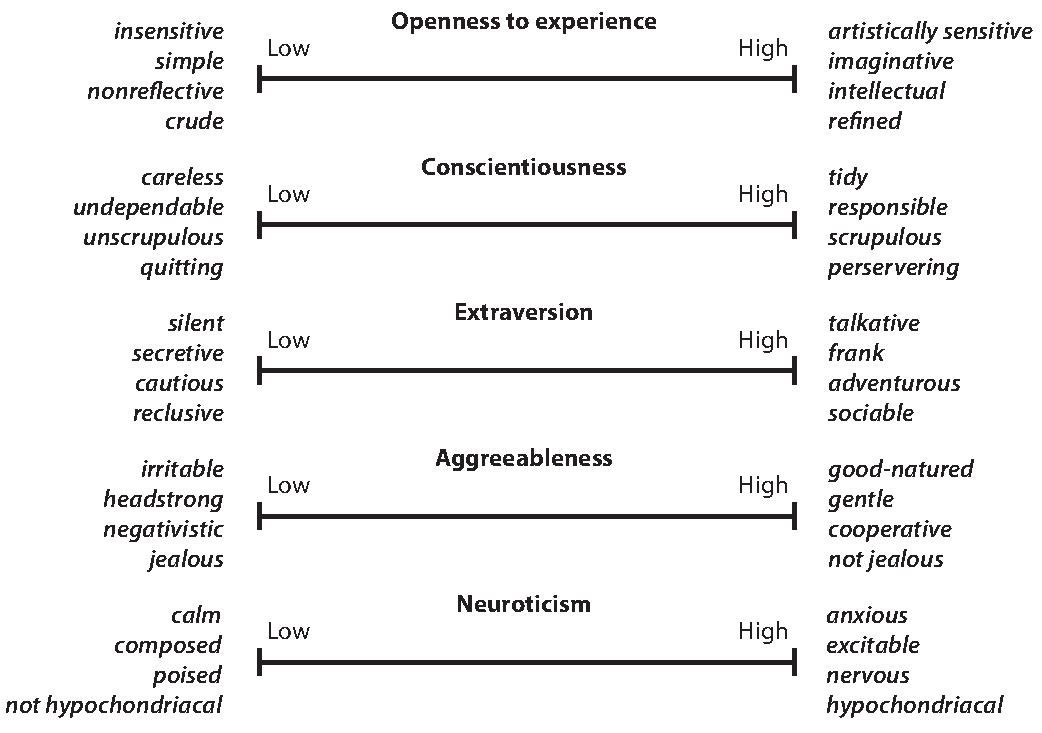
\includegraphics[width=\linewidth]{figures/bigfive}
\caption{\label{fig:bigfive}Visualization of the BFM. Traits are shown in the order 'OCEAN', each constituting a continuous domain between low trait value, associated with adjectives that oppose the name of the trait, and high trait value, associated with adjectives that support the trait name. The model explains an individual's personality as a vector with one score per trait. Scored are typically obtained through a questionnaire inventory.}
\end{figure}

Human efforts to derive a taxonomy for character traits predate our calender. Early efforts include the four \textit{Cardinal Virtues} - prudence, temperance, courage and justice - due to Plato and Aristotle\mcite{Broadie1991-BROEWA}, as well as the four humors - blood, yellow bile, black bile and phlegm - said to have originated in Ancient Egyptian medicine but formalized by Hippocrates\mcite{lloyd1978hippocratic}.
The foundation of the field now known as \textit{trait theory} is, however, not considered rooted in this way thinking. Rather it started in 1884 when Sir Francis Galton established the \textit{lexical hypothesis} which states that any trait that is truly important to humans will become encoded into their language\mcite{galton1949measurement}. Galton reported finding exactly 1000 personality descriptive adjectives in the English language. A similar effort was later made by Gordon Allport and Henry Odbert (1936) using the \textit{Webster's Unabridged Dictionary} (2nd Ed.), which resulted in a 17,953 long list of unique words to describe personality and behavior\mcite{allport1936trait}. The first effort to understand the underlying structure of this vocabulary was taken by Raymond B. Cattell (1943) who applied factor analysis to the covariance structure of words when used to describe individuals in large test groups, and found 16 primary and eight secondary traits\mcite{cattell1945description}. This result was refined by Donald. M. Fiske (1949) who, in an effort to replicate Cattell's result, arrived at a five factor solution\mcite{digman1990personality}. Supported by later research, this is still the prevailing result. It was coined the \textbf{Big Five model}\footnote{Also commonly referred to as the Five Factor model (FFM).} (BFM) by Lewis Goldberg (1981)\mcite{goldberg1981language}, but credit for its invention is typically given to Fiske\mcite{fiskepersonality}. The model is shown in Figure \ref{fig:bigfive}. It offers five high-level personality traits: \textit{openness to experience} (\OPE), \textit{conscientiousness} (\CON), \textit{extraversion} (\EXT), \textit{aggreeableness} (\AGR) and \textit{neuroticism} (\NEU)\mcite{920817074619920601}, which are typically recalled using acronyms OCEAN or CANOE. Traits in the BFM is typically measures using a questionnaire inventory such as the Big Five Inventory or the IPIP100 Inventory which relies on honest self-report by the subject\mcite{IPIPwebsite}. Rather than reducing the rich tapestry of the human psychology to mere five traits, the model seeks to provide a compelling framework for organizing the enormous variety of psychological differences characterizing humans. It assumes a hierarchical view of psychological traits, where the Big Five traits (BFT) are independent roots that each branch into many facets and subfacets.

\subparagraph*{Criticism} The BFM is widely accepted among a substantial number of researchers, by some even considered a universally valid structure that transcends culture and language\mcite{bouchard2001genes, mccrae1997personality}. Unsurprisingly this particular viewpoint is not unchallenged. Recent findings have shown the BFM to only explain variance in a subset of traits (\CON, \EXT, \NEU) for indigenous societies\mcite{gurven2013universal}, which resonates with the finding that \textit{humility} emerges as a trait when studying populations in Asia (as captured by the HEXACO model, see below). Furthermore the lexical hypothesis has been argued to have the two following problems: (1) since language itself is not developed by experts, the inherent ambiguity of words causes any model based on language sampling to, at best, reflect only a lay perceptions of the traits\mcite{cervone2007a, westen1996model}, and (2) words can't accurately capture the spectrum of personality because some very important traits are tacit\mcite{argyle1973a}.

\subparagraph*{Limitations} It has been shown that the BFM only captures up to 56\% of a persons personality spectrum\mcite{boyle1995measurement}. This is very important knowledge to have when using the BFM in any study that attempts to make general statements about personality. In the current undertaking, it too must be respected that certain fine-grained aspect of personality won't be captured and therefore shouldn't be speculated about. Unlike the Eysenck model (presented below) the BFM doesn't for example capture personality variance due to \textit{psychotism}. It thus stands to reason that any strategies inferred from a dataset of BFTs cannot possibly be purely psychopathy, although it is in fact a proven evolutionarily stable strategy (ESS, see Section \ref{subsubsec:individualDifferencesAndPersonality})\mcite{workman2014evolutionary}.

\subparagraph*{Alternative models} While the BFM is the most commonly used system for measuring personality traits, it is not the only one. The HEXACO model of personality structure is another widely accepted model which has deeper roots in European and Asian languages. Using factor analysis it finds six traits, where five are similar to those in the BFM, and one is related to honesty and humility\mcite{ashton2004six}. Another important model is Cattell's 16PF questionnaire which measures personality on 16 out of his original 24 personality dimensions\mcite{cattell2008sixteen}. Finally, the Eysenck personality questionnaire reduces personality into mere three traits: \textit{psychoticism},	\textit{extraversion} and \textit{neuroticism}. In this model psychoticism captures the aggressive and more extreme nuances of neuroticism. Rather than capturing a wide spectrum of personality the Eysenck model aims only at capturing personality variance associated with temperament.

		\subsubsection{How does evolutionary psychology treat personality? \label{subsubsec:individualDifferencesAndPersonality}}
		Evolutionary psychologists are interested in personality because there are clues that suggest it might play an important role in natural selection. The first such clue is that much research shows personality to exhibit stability over time and contexts\mcite{cooper2015individual, larsen2008personality, buss2009can}. The second is that studies have shown individual personality traits to be $30-50\%$ inherited\mcite{newman1998individual, THG:8492454}. This strongly suggests that there are fitness benefits to different genetically inheritable aspects of personality.
EP suggests that due the heredity of personality it may be seen, from an evolutionary point of view, as \textbf{a type of behavioral strategy}, i.e. a motivational system which predisposes people to seek out particular situations and respond in particular ways\mcite{workman2014evolutionary}.
This argumentation, however, gives rises to a paradox: in trying to explain the heredity of personality traits by assuming that the traits increase fitness, the question of why personality is \textit{only} $30-50\%$ genetic must be addressed.
EP has several theories to explain this, of which the two central ones are: (1) the brain develops as it does due to \textit{chance} because the genome only contains \textasciitilde20,300 genes of information which cannot possibly code exactly for a brain that has \textasciitilde100 billion complexly interacting neurons and (2) the individual is born with an adapted capacity for environmental calibration because inherent uncertainty of the world renders a fixed strategy on birth suboptimal\mcite{workman2014evolutionary}.

% Personality is treated as a strategy in large part because it conveniently explains empirical observations, but there are no and as such it should be considered a \textit{hypothesis}, which is a notion that should be respected when using this view as a basic assumption for further research. In fact, key founders of EP, Leda Cosmides and John Tooby, argued in an early paper (1990) that heritable individual differences are simply noise irrelevant to the basic functioning of the psychological machinery, similar to how the color of wires in a car engine have no effect on the actual functioning of the car\mcite{tooby1990universality}. This view has changed today. High-profile evolutionary psychologist and linguist Stephen Pinker openly talks about personality as strategy in his acclaimed book \textit{How The Mind Works} (1999}\mcite{pinker1999mind}, and the most cited personality researchers in EP David Buss and Daniel Nettle are firmly dedicated to this view\mcite{buss2009can, nettle2006evolution}.

EP's primary instrument for measuring personality is the BFM because, as argued by Buss, it represents the most evolutionarily plausible way of carving up human personality\mcite{buss1991evolutionary, larsen2008personality}. The main reason for this is because the traits are orthogonal and they capture a wide array of individual differences. To compare, in one end of the scale Cattell's 16PF model elaborately cover many aspects of personality at the cost of using a very non-orthogonal system of traits, whereas in reverse the Eysenck model is too narrow and disregards evolutionarily important traits like \textit{agreeableness}, \textit{conscientiousness} and \textit{openness to experience}.

% Trade-offs
\subparagraph*{Trade-offs cause trait variations}
Trade-offs between physical and psychological traits are inherent to almost all biological systems. It can be understood intuitively as the problem of having to choose between things that are good for something but can't be had simultaneously. Like being big or small: each has advantages, but obviously an organism must somehow choose to be either like one or a \textit{trade-off}. An investigated example from Darwinian evolutionary theory explains the practical value of this problem. 
Ground finches on the Galapagos are typically sectioned into three types: (1) long beak/medium body, (2) large thick beak/large body and (3) small thick beak/small body. Shoval et. al. shows that each of these trait configurations are in fact archetypes of traits exhibited by all ground finches, and that each archetype is optimized to perform a specific task (see Figure \ref{fig:trade_offs_finch_paretoOptimality}.b)\mcite{shoval2012evolutionary}. Archetype-(1) is optimized for picking insects and extracting nectar, archetype-(2) is optimized for cracking large hard seeds and archetype-(3) is optimized for crushing small soft seeds. Shoval et. al. observes that most ground finches are, however, not exactly like any archetype, rather each seems to \textit{trade off} archetypal traits such as to be able to perform all tasks to some ability. This is thought to be a strategy for coping with changing ecological pressures, such that when a niche becomes unavailable (e.g. small soft seeds disappear) the organism has other ways of leveraging its fitness.

\begin{figure}[ht]
	\centering
	\textbf{a)}
	\hspace{0.2cm}
	\begin{minipage}[r]{0.4\textwidth}
		\centering
		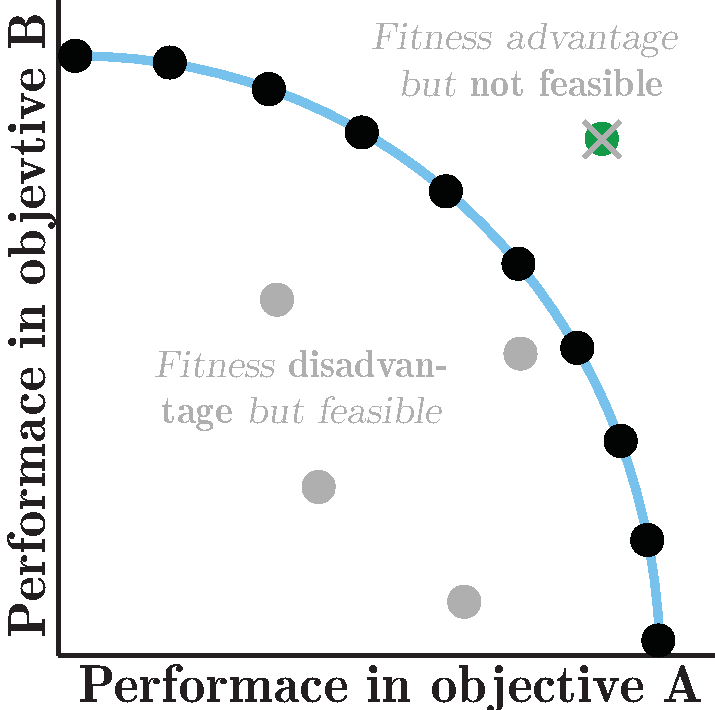
\includegraphics[width=1\textwidth]{figures/paretoOptimality}
	\end{minipage}
	\hspace{0.7cm}
	\textbf{b)}
	\hspace{0.2cm}
	\begin{minipage}[l]{0.4\textwidth}
		\centering
		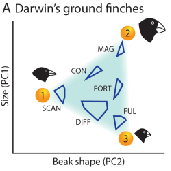
\includegraphics[width=1\textwidth]{figures/trade_offs_finch}
	\end{minipage}
	\caption{\label{fig:trade_offs_finch_paretoOptimality} \textbf{a)} Illustration of distribution of points in a two-objective performance space where the black points are Pareto optimal and the blue curve signify the Pareto front where no objective can be optimized further without decreasing performance in the other. \textbf{b)} Illustration of how members of a species is distributed in trait-space to respect trade-offs between archetypal traits (source: Shoval et. al.\cite{shoval2012evolutionary}).}
\end{figure}

It is reasonable to ask what the best trade-off configuration of traits is, but the immediate answer is that there are infinite. To explain what this means, the concept of \textit{Pareto optimality} must be introduced. Pareto optimality is a concept that stems from Economics and characterizes the set of solutions to a multi-objective optimization problem where no objective can be further optimized without having to compromise performance of another. For two objectives this means that solutions that are Pareto optimal are distributed along a curve in performance space, as illustrated in Figure \ref{fig:trade_offs_finch_paretoOptimality}.a. For an individual organism, traits will be adopted in such a way the the organism remain Pareto optimal, i.e. good enough at all evolutionarily important tasks to remain fit. Those that are not on the Pareto front will have a fitness disadvantage and be selected against in the long run, thus not passing on the genes that caused the disadvantage. The propensity to seek niches of least competition, i.e. \textit{Niche filling}, drives populations to distribute traits somewhat evenly across the Pareto front.

The configuration of traits that a ground finch inherits from its parents can, in an evolutionary view, be considered a \textit{strategy} for coping with the environment. This view is conceptually similar to the way evolutionary psychologists treat personality. For this reason, an individuals configuration of personality traits is also considered to be under influence of trade-offs. For example a person cannot (disregarding personality disorders) be both extroverted and introverted at the same time, and if life in general can be viewed as a complex collection of tasks then a persons level of intro-/extraversion poses an evolutionary trade-off problem just as much as beak shape does to seed-cracking.

\subparagraph*{Frequency dependence drives emergence of multiple strategies}
EP treats the predominance of different personalities/behavioral strategies using the concept of \textit{frequency dependence} from evolutionary theory. It argues that the reason why all humans have not simply adapted the \textit{single best strategy} is that, while at times there may be one strategy which is the best, this quickly changes when too many individuals adopt it. This can be compared to how driving to work early is a good strategy for avoiding traffic as long as not too many people do it. Another example is that of \textit{psychopathy}. Workman et. al. argues that psychopathy is in fact (purely evolutionarily speaking) a very effective behavioral strategy to maximize personal fitness \footnote{Also: \textit{exclusive fitness} - only increasing fitness of self as opposed to \textit{inclusive} fitness which measures fitness of all kin.}, provided there are not too many psychopaths around\mcite{workman2014evolutionary}. In most populations only 1-3\% of individuals will adopt this strategy to a sub-clinical level whereas clinical psychopathy is as low as 0.2\%\mcite{kring2005abnormal}. The psychopath strategy revolves around gaining peoples trust and then using them for own goals, and imaginably this strategy wouldn't work well if there were so many psychopaths that otherwise trusting people were used to getting cheated by psychopaths and therefore in general learned only to trust kin or long-term friends.

\newcommand*\rot{\rotatebox{90}}
\newcommand*\OK{\ding{51}}
\newcommand{\lbo}[1]{\multicolumn{1}{|c|}{#1}}
\newcommand{\rbo}[1]{\multicolumn{1}{c|}{#1}}
\newcommand\Tstrut{\rule{0pt}{4ex}}
\newcommand\Bstrut{\rule[-1.9ex]{0pt}{0pt}}
\newcommand{\playerA}{\multirow{2}{*}{\rotatebox{90}{\textbf{You}}}}
\begin{table}
	\vspace{-0.75cm}
	\centering
	\begin{minipage}[l]{0.49\textwidth}
		\hspace{-0.5cm}
		\begin{tabular}{R{0.1cm}C{0.9cm}C{1.5cm}C{1.5cm}}
			{} 		& {}	& \multicolumn{2}{c}{\textbf{Opponent}} \vspace{0.15cm}\\
			{} 		& {}	& \multicolumn{1}{C{1.5cm}}{Hawk}& 	\multicolumn{1}{C{1.5cm}}{Dove}	\\ \cline{3-4}
			\playerA& Hawk	& \lbo{$(V-C)/2$} 	& \rbo{$V$} 	\Tstrut\Bstrut					\\ \cline{3-4}
			{} 		& Dove	& \lbo{0} 			& \rbo{$V/2$} 	\Tstrut\Bstrut\Bstrut			\\
			\cline{3-4}
		\end{tabular}
	\end{minipage}
	\hspace{0.1cm}
	\begin{minipage}[r]{0.45\textwidth}
		\vspace{1.4cm}
		\caption{\label{tab:prisoners_dilemma} Reward table for the hawk-dove game. It models an exchange between 'you' and an opponent where each chooses e.g. to be like a dove (cooperate) or hawk (cheat). Each combination of moves has a different reward for each player.}
	\end{minipage}
	\vspace{-0.25cm}
\end{table}

\subparagraph*{Game theory can explain some behavioral strategies}
The suggestion that personality is a behavioral strategy must be understood in terms of what evolutionary psychologists already identify with the term 'strategy'. It has its roots in the field of game theory, which examines how people behave depending on the strategies of others. Here the term is simply synonymous with \textit{algorithm}. A central goal of applying game theory is to find a strategy for an individual which, given what everybody else is doing, cannot make the individual better off. Such as strategy is said to represent a state of \textit{Nash Equilibrium}. A commonly treated paradigm is the so-called \textit{hawk-dove game} which is illustrated in Table \ref{tab:prisoners_dilemma}.
It models an interaction between two players, \textit{you} and an \textit{opponent}, who have to share a resource $V$. Each player can choose to cooperate or defect, i.e. act as a \textit{dove} or as a \textit{hawk}. If both cooperates $V$ is shared equally, but if one chooses to cooperate while the other doesn't the gullible player gets nothing while the defector gets all. In case both players choose the hawk-strategy the resources are shared equally but at the cost of battle, $C$. This game has been studied extensively, and for repeated games - between rational players - the winning strategy is a so-called \textit{tit-for-tat} strategy\mcite{workman2014evolutionary}, where one simply copies the opponents' last move. This strategy constitutes a Nash equilibrium because, provided the opponent doesn't change strategy, there is nothing to gain from changing strategy\mcite{nash1950equilibrium}. Other strategies such as a \textit{generous-tit-for-tat} which chooses cooperation with some probability even if the opponent has defected, or \textit{win-stay lose-shift} which (even simpler) just repeats past moves if they were successful and tries something new if not, have been shown to work slightly better when the opponent acts irrationally\mcite{nowak2006five}. Other less sophisticated strategies which are not in equilibrium are \textit{uncompromising cooperation} as well as \textit{constant defecting}.

A generalization of the Nash equilibrium to describe evolutionary stability which is used in biology, behavioral ecology and EP is the concept of the evolutionarily stable strategy (ESS). An ESS is a behavioral strategy that, if it exists abundantly enough in a population, it cannot be replaced by an invading strategy\mcite{smith1974theory}. It links to the concept of frequency dependence examined above, when multiple ESSs exist alongside, because they depend on each other in complex ways (recall the example with psychopathy), and can therefore be said to be \textit{inter}-frequency dependent (this terminology is not used in literature but resonates with notions raised by Workman et. al.\mcite{workman2014evolutionary} and Buss \mcite{buss2009can}).

EP considers a number of behavioral strategies to be ESS. Firstly the psychopathy strategy is thought to be ESS. Another is \textit{reciprocal altruism} which has been extensively studies in tribe cultures\mcite{workman2014evolutionary}, where individuals tend to give presents to non-kin with the expectation that presents will be returned to them at another time of greater need. Reciprocal altruism is formally treated as either: (1) \textit{direct} where reciprocity is expected from the same person/group and of equal value as was donated (compared to the tit-for-tat strategy) or (2) \textit{indirect} which relies on good reputation, established through gossip of altruistic acts, to eventually provide the giver with resources from like-minded (cooperation strategy)\mcite{nowak2006five}.
Another important strategy which is thought to be ESS is the \textit{freeloader}, which utilizes the cooperators trusting nature to cheat as frequently as possible within the limit of remaining an ESS. Evolutionary psychologists speculate the \textit{freeloader} to have significant importance to community formation through exemplifying morally wrong behavior\mcite{workman2014evolutionary}.

% \textbf{Individual personality is a trade-off between fundamental strategies}.
% To fully adapt one fundamental strategy is rarely a robust solution due to the fitness fluctuations that result from frequency dependence.
% An individual will therefore tend to adopt a strategy that is a mix of many fundamental strategies.
% This can be thought of as a multi-objective optimization problem: individuals must ensure maximal fitness but adopted strategies must obey inherent trade-offs between performance of fundamental strategies.
% It confines solutions to a surface in performance space called the \textit{Pareto front}.
% The Pareto front defines the boundary where increasing performance in one strategy comes at the expense of performance in others.
% Evolution tends to not allow individuals to stay off the Pareto front because their fitness advantage would be inferior to those on it, and as such personalities of people should be confined to the Pareto front where they remain \textit{Pareto optimal} trade-offs between fundamental strategies.

	% Pareto Task Inference
	\newpage
	\subsection{Pareto Task Inference \label{subsec:paretoTaskInference}}
	Pareto Task Inference (ParTI) is a research paradigm developed at the Uri Alon lab to solve a number of problems related to evolution of morphology in various species. ParTI has been applied to understand systems in biology involving cancer cells\mcite{hart2015inferring}, morphology of ammonite shells\mcite{tendler2015evolutionary}, mass and longevity design of mammals\mcite{szekely2015mass}, and more\mcite{korem2015geometry, shoval2012evolutionary}. It is founded in principles relating to evolutionary trade-offs and Pareto optimality as explained in Section \ref{subsubsec:behaviorAndPersonality}, and combines these to provide a novel approach for inference of biological functions.

The goal of ParTI is to infer the \textit{evolutionary objectives} of an organism. Objectives can be anything from \textit{tasks} like cracking nuts and picking insects which a finch must perform well to remain evolutionarily fit, or even behavioral \textit{strategies} that a human can employ to perform all of life's evolutionarily important tasks in a way that maximizes fitness in a given niche. \textbf{The value proposition of ParTI is that it provides evidence of what these objectives are only by considering the traits of the organism in question}. ParTI works in two parts:
\begin{itemize}[leftmargin=.55in]
	\item [\textbf{\ref{subsubsec:ParTIptOne}}] Find archetypes, i.e combinations of traits that are optimized for specific objectives (\textit{Pareto}).
	\item [\textbf{\ref{subsubsec:ParTIptTwo}}] Infer objectives by studying the combinations of traits for each archetype (\textit{Task Inference}).
\end{itemize}

The central paradigm of ParTI exists in the first part, while the second part employs statistical methods to produce scientific results. In the following, each of these are examined.

		% Finding archetypes in trait-space
		\subsubsection{Finding traits that are optimized for objectives \label{subsubsec:ParTIptOne}}
		This part of ParTI is based on two core abstractions:
\begin{enumerate}
	\item Inherent trade-offs between traits that are evolutionarily important to increase performance in different objectives, drive variation in a population to distribute along a Pareto front.
	\item The Pareto front in trait-space is the hypervolume of a simplex. Each vertex of this simplex represents combinations of traits that are optimal for performing its respective objective.
\end{enumerate}
From (2) it is noted that vertices of a simplex may also be treated as \textit{archetypes}. Abstraction-(1) is explained in Section \ref{subsubsec:individualDifferencesAndPersonality}. Abstraction-(2) requires further explanation. When organisms have a single performance objective natural selection leads to traits that maximize performance of that objective. Any deviation from the optimal trait configuration causes performance, and thus fitness, to drop and in turn individuals who fall too far from the optimum will be selected against. This is illustrated in Figure \ref{fig:objectivePerformance}.a. When multiple objectives exist, no set of traits can optimize performance in all tasks and as such organisms must trade off traits relating to optimal performance of each objective. In Figure \ref{fig:objectivePerformance}.b a performance function of three objectives is illustrated. It shows that in order to maximize performance, leaving the triangle spanned by the three peaks is disadvantageous. In fact, it corresponds to moving away from a position of Pareto optimality since performance in each objective is decreased without any gain. Therefore, the triangle shaped by the peaks, or \textit{archetypes}, constitutes the region where traits are Pareto optimal, i.e. the Pareto front.
Figure \ref{fig:paretoFront} shows how the number of objectives shapes the Pareto front. If there are two tasks, organisms must have traits that are distributed somewhat along a line between the archetypes in order to remain Pareto optimal, and if there are four tasks the Pareto front will be the volume spanned by the corresponding four archetypes shaping a tetrahedron.
This is important because it shows if objectives are \textit{evolutionary tasks} or \textit{behavioral strategies}, these can be inferred just by considering the vertices of the triangle, i.e. the archetypes that emerges from the distribution of points in trait-space.

\begin{figure}
	\centering
	\textbf{a)}
	\begin{minipage}[l]{0.40\textwidth}
	\centering
		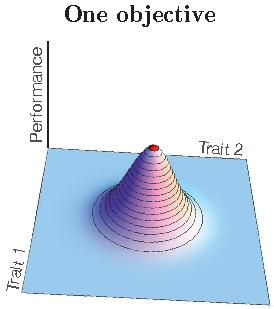
\includegraphics[width=\textwidth]{figures/objectivePerformance}
	\end{minipage}
	\textbf{b)}
	\hspace{0.2cm}
	\begin{minipage}[r]{0.40\textwidth}
		\centering
		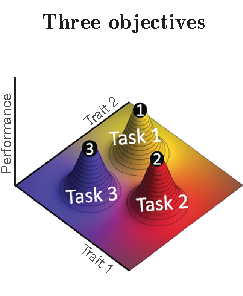
\includegraphics[width=\textwidth]{figures/objectivePerformance3}
	\end{minipage}
	\caption{\label{fig:objectivePerformance} \textbf{a)} Performance function of a single objective/task in trait-space (source: \cite{sheftel2013geometry}. \textbf{b)} Performance function of three objectives/tasks in trait-space. Archetypes are the local maxima (source: \cite{szekely2015mass}).}
\end{figure}

\begin{figure}[h]
\centering
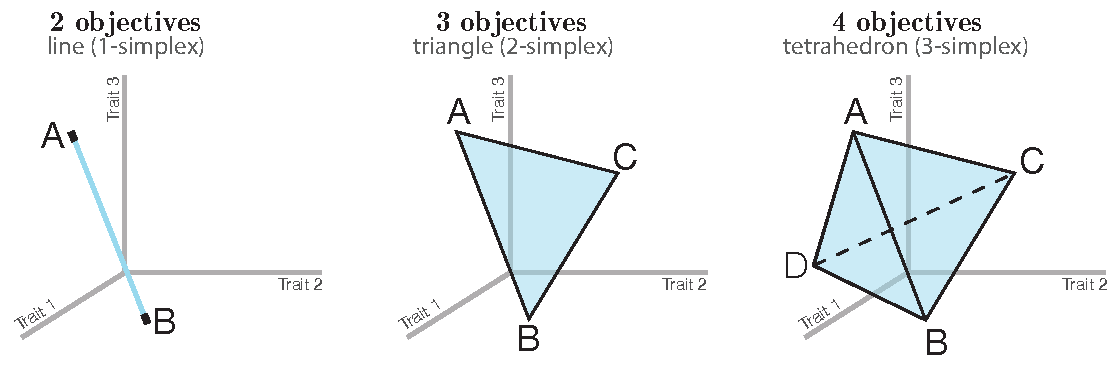
\includegraphics[width=\linewidth]{figures/paretoFronts} 
\caption{\label{fig:paretoFront} Pareto front regions (blue) for up to three objectives in trait-space. In the \textbf{2 objectives}-case the Pareto front spans the edge connecting objectives A and B. For \textbf{3 objectives} and \textbf{4 objectives} Pareto fronts are the area and volume, respectively, of the simplex spanned by the set of objectives.}
\end{figure}

\begin{figure}
	\centering
	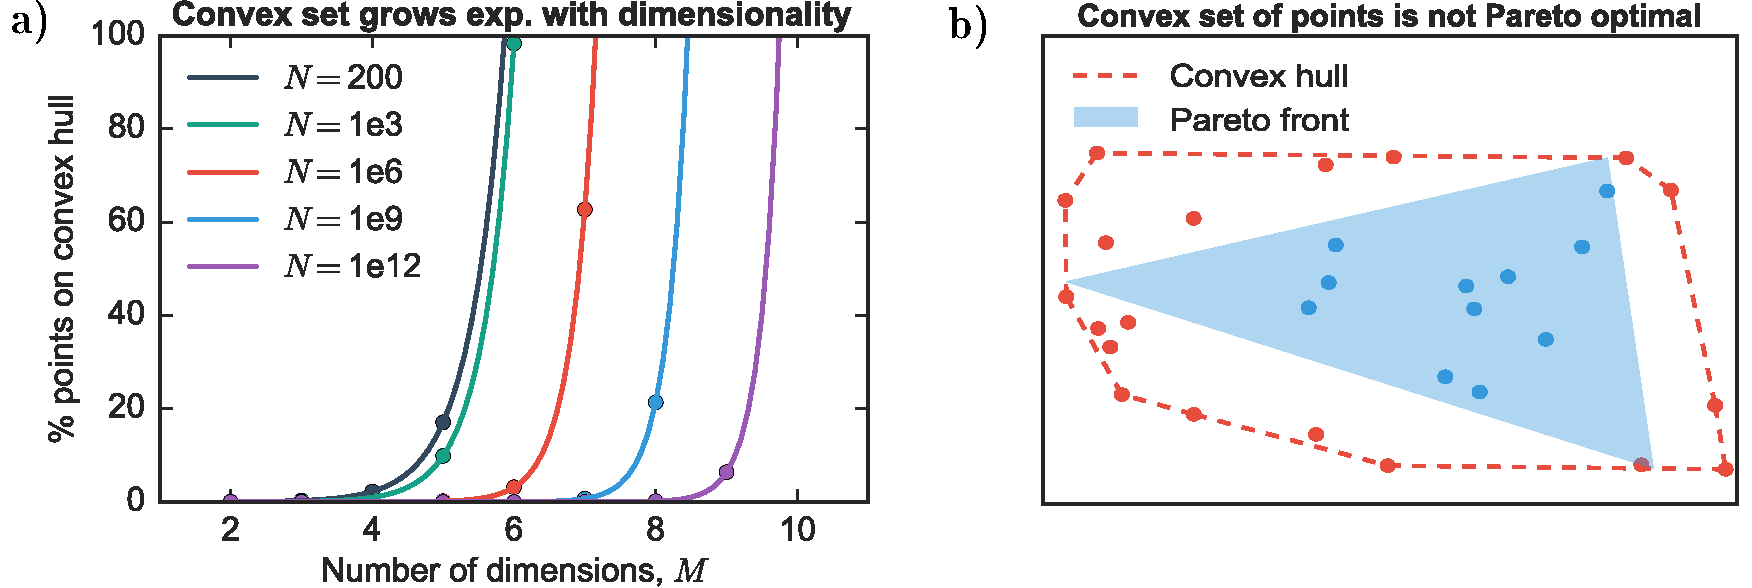
\includegraphics[width=1\textwidth]{figures/convexHullCurseOfDimensionality}
	\caption{\label{fig:convexHullCurseOfDimensionality} \textbf{a)} The size of the convex hull for $N$ points scale exponentially with the number of dimensions $M$ as $\mathcal{O}(\log{}n)^{M-1}$. Above five dimensions, many points are required in order to obtain a low ratio between the size of the convex set and the number of points. Note that the $M-$axis is discrete and that curves are plotted on a continuous scale for the sake of illustration. \textbf{b)} The Pareto front is a simplex anchored in $d+1$ points on the convex hull, and as such points on the hull that are not archetypes are not Pareto optimal.}
\end{figure}

\subparagraph*{The ParTI principle generalizes to any number of dimensions}
Since a triangle is just a special case of a $d$-simplex composed of $d+1$ vertices, the ParTI principle can be used to infer objectives in any number of dimensions. However, ParTI provides no "idiot-proof" solution to any dataset. For very high-dimensional data like gene expressions which may span a thousand dimensions, one shouldn't expect to find a thousand and one objectives. There is a purely mathematical reason for this. The convex set for any distribution of points grows exponentially with the number of dimensions as $\mathcal{O}(\log{(n)}^{M-1})$\mcite{morup2012archetypal}. Points on the convex hull are more likely to be outside of the Pareto front, and as such the possibility of finding valid simplex geometries (where \textit{valid} means that most points are on the Pareto front) in high-dimensional spaces is severely diminished. Figure \ref{fig:convexHullCurseOfDimensionality} illustrates that for over five dimensions, a very large number of datapoints are required to maintain a low ratio between the number of points in the convex set to the number of points in total.

Is this problematic? Somewhat yes, but recall from Section \ref{subsubsec:individualDifferencesAndPersonality} the concept of ESS. In most biological systems multiple ESSs can only exist alongside if they are frequency dependent and \textit{inter}-frequency dependent, and arguably there must be an upper limit to the number of complexly interacting strategies which can be ESS and exist alongside. That said, the above analysis cannot inform us about where this limit lies as biology has little regard for computational shortcomings.

\subparagraph*{Projections enable inference in high-dimensional data}
There is a solution to the problem pointed out above and illustrated in Figure \ref{fig:convexHullCurseOfDimensionality}. In high-dimensional systems such as cancer cells which are typically measured in terms of their gene expressions, objectives can be found using dimensionality reduction methods. In ParTI literature the prevailing such method is principle component analysis (PCA)\mcite{hart2015inferring}. PCA allows the analyst to project points in a high-dimensional space onto a subspace spanned an orthogonal basis of vectors which explain the most variance in the data. These vectors are called principle components (PC) and are computed as the eigenvectors of the covariance matrix. Informally, PCA can be thought of as casting a shadow of an object in such as way that the object can best be recognized. If the object was a sword, the first PC would follow the length of the sword and the second (being orthogonal to the first) would follow the guard and as such the best way to show that is was a sword just from looking at the shadow would be to project it onto these two components.

For objects that exist in high-dimensional spaces such as a point-cloud of gene expressions this method of "casting the shadow of highest explained variance" works methodically in exactly the same way as the sword example. Here, however, the analyst has more freedom to choose the dimensionality of the space projected to (the shadow). When ParTI treats high-dimensional data it looks for shadows that are shaped like simplexes (see Figure \ref{fig:paretoFront}}). For a low-dimensional projection where the points appear to fall inside a simplex, the vertices can be taken as the combinations of traits that allow for optimal performance of objectives, and each can in turn be identified by further analysis into how organisms with that combination of traits behave.

		% Inferring objectives from enrichment near archetypes
		\subsubsection{Inferring objectives from enrichment near archetypes \label{subsubsec:ParTIptTwo}}
		In the current context the word \textit{inference} simply means to uncover evidence of certain features or behaviors of an archetype to the point where it is valid to make an interpretation of what the main objective of the archetype is. As such, ParTI is really a method for \textit{providing evidence} rather than giving an ultimate answer.

Since archetypes in trait-space are optimal configurations of traits for performing specific objectives that are evolutionarily important, the problem of inferring what those objectives are can be solved in many ways. For very simple systems one could unobtrusively observe how organisms employ their traits and take special notice of behavioral differences between those that resemble archetypes\mcite{shoval2012evolutionary}. But for systems that can't be directly observed, other methods must be used. A relevant example is personalities of people and which behavioral strategies for performing evolutionarily important tasks they lead to. In this example traits are personality factors such as the Big Five (see Section \ref{subsubsec:dimensionsOfPersonality}) and the objective is the behavioral strategy that the personality is optimized to perform. Given the archetypes it would be to time-consuming and obtrusive to monitor people, who were similar to each archetype, in their natural habitat. Using qualitative interviewing might work better but would also be time consuming and possibly introduce qualitative research biases.

A better approach is to study the statistical properties of individuals who are similar to each archetype. Using \textit{extra data} such as demographic variables, response items from surveys and behavioral data, layers of information can be added such as to reveal what people similar to each archetype typically do for a living, whether they tend to be married or what age range they occupy. This approach is general. If the system were cancer cells and traits were gene expressions, extra data such as tissue type, cell cycle period and protein production level would provide evidence to aid inference of objectives for different cells\mcite{hart2015inferring}.

There are different methods for doing this. The simplest method is to correlate the feature value with distance from the archetype and then use the slope and correlation coefficient as measures of relatedness.
Another approach which provides a better visual image is to analyze the \textit{enrichment} of features near the archetypes. As illustrated in Figure \ref{fig:enrichmentExample} this method works by binning points according to their distance from the archetype and then taking the average of the feature in each bin to create a curve which shows whether the feature tends to be enriched or \textit{depleted} near the archetype. If the feature is categorical the method estimates the frequency of each category in every bin, such as to create separate histograms for the feature-categories. This method is applied widely in ParTI literature\mcite{korem2015geometry, szekely2015mass, tendler2015evolutionary, shoval2012evolutionary, hart2015inferring}.

\begin{figure}
	\centering
	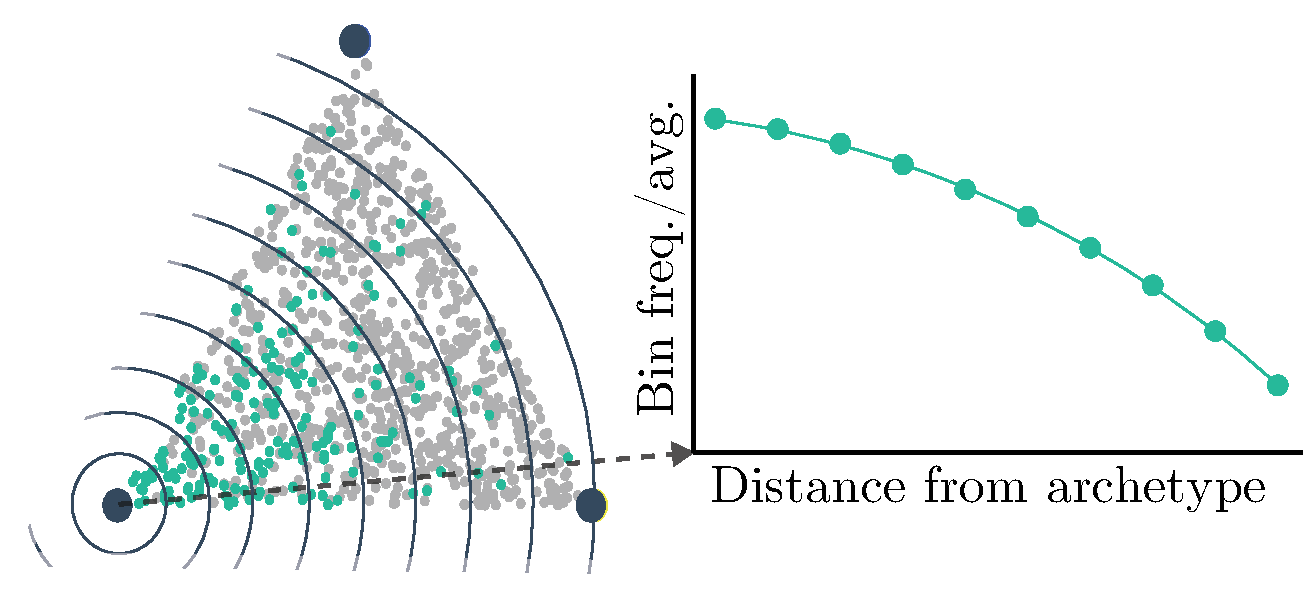
\includegraphics[width=0.7\textwidth]{figures/enrichmentExample}
	\caption{\label{fig:enrichmentExample} Enrichment of variables near archetypes are estimated across a number bins characterized by distance to the archetype. If the studied feature is continuous the }
\end{figure}

		% Archetypal Analysis
		\subsubsection{Inferrence of archetypes \label{subsubsec:archetypalAnalysis}}
		So far \textit{archetype} has been used synonymously with \textit{simplex vertex}, and surely simplex vertices can be considered archetypes - but archetypes are not necessarily simplex vertices. Figure \ref{fig:AA} gives two examples of archetypes in clusters of simulated points, and shows that archetypes are in fact just the intuitive "corner-points" of any point cloud.
The method for inferring these corner-points is called archetypal analysis (AA). It was introduced by Adele Cutler and Leo Breiman in 1994 and developed as an unsupervised learning method for clustering data that is not well-separated\mcite{cutler1994a}. The central idea it to derive a set of archetypes from which all points can be approximated as linear combinations. Below is given a brief introduction to the method.

\subparagraph{The AA factorization problem}
AA solves the following matrix factorization problem. Consider a data matrix $\matr{X} = [\matr{x}_1, \matr{x}_2, ..., \matr{x}_n] \in \mathbb{R}^{m \times n}$. The task of AA is to estimate the two factor matrices $\matr{S} \in \mathbb{R}^{k \times n}$  and $\matr{C} \in \mathbb{R}^{n \times k}$ such as to satisfy the following equation with minimal approximation:

\begin{equation}
	\matr{X} \approx \matr{AS} = \matr{XCS}
	\label{eq:AA}
\end{equation}

The number of archetypes is controlled by $k$ and can be chosen by the analyst, while the archetypes themselves are column vectors in $\matr{A} \in \mathbb{R}^{m \times k}$. $\matr{C}$ and $\matr{S}$ are column stochastic matrices subject to $|\matr{c}_j|_1 = |\matr{s}_i|_1 = 1$. Columns in $\matr{C}$ give the coefficients of each archetype as a linear combination of the data points, and reversely $\matr{S}$ give the coefficients of each data point as an approximate linear combination of the archetypes. This leads to the property that archetypes may be derived from data points as $\matr{A} = \matr{XC}$ and data points approximated from archetypes as $\matr{X} \approx \matr{AS}$. This introduces symmetry into the matrix factorization problem consistent with the following statement: \textit{archetypes are convex combinations of the data points and data points are approximated by convex combinations of archetypes}. $\matr{C}$ and $\matr{S}$ are derived by minimizing the residual sum of squares ($RSS$):
\begin{equation}
	RSS = \|\matr{X} - \matr{XCS}\|_F^2
	\label{eq:AALossFunction}
\end{equation}
subject to $|\matr{c}_j|_1 = 1\,\, \forall \,\, j \in \{0, ..., k\}$ and $|\matr{s}_i|_1 = 1 \,\, \forall \,\, i \in \{0, ..., n\}$, where $\| \cdot \|_F$ is the Frobenius norm. Furthermore, AA imposes the constraint that all coefficients of $\matr{C}$ and $\matr{S}$ are greater or equal to zero. Note that $RSS$ goes to zero in the limit $\matr{AS} \rightarrow \matr{X}$ where the data points can be  reconstructed exactly as convex combinations of the archetypes. It can be shown that Equation \eqref{eq:AALossFunction} is non-convex, and that the optimization problem has no closed form solution\mcite{cutler1994a}, yielding numerical methods necessary for solving the problem.

\begin{figure}
	\centering
	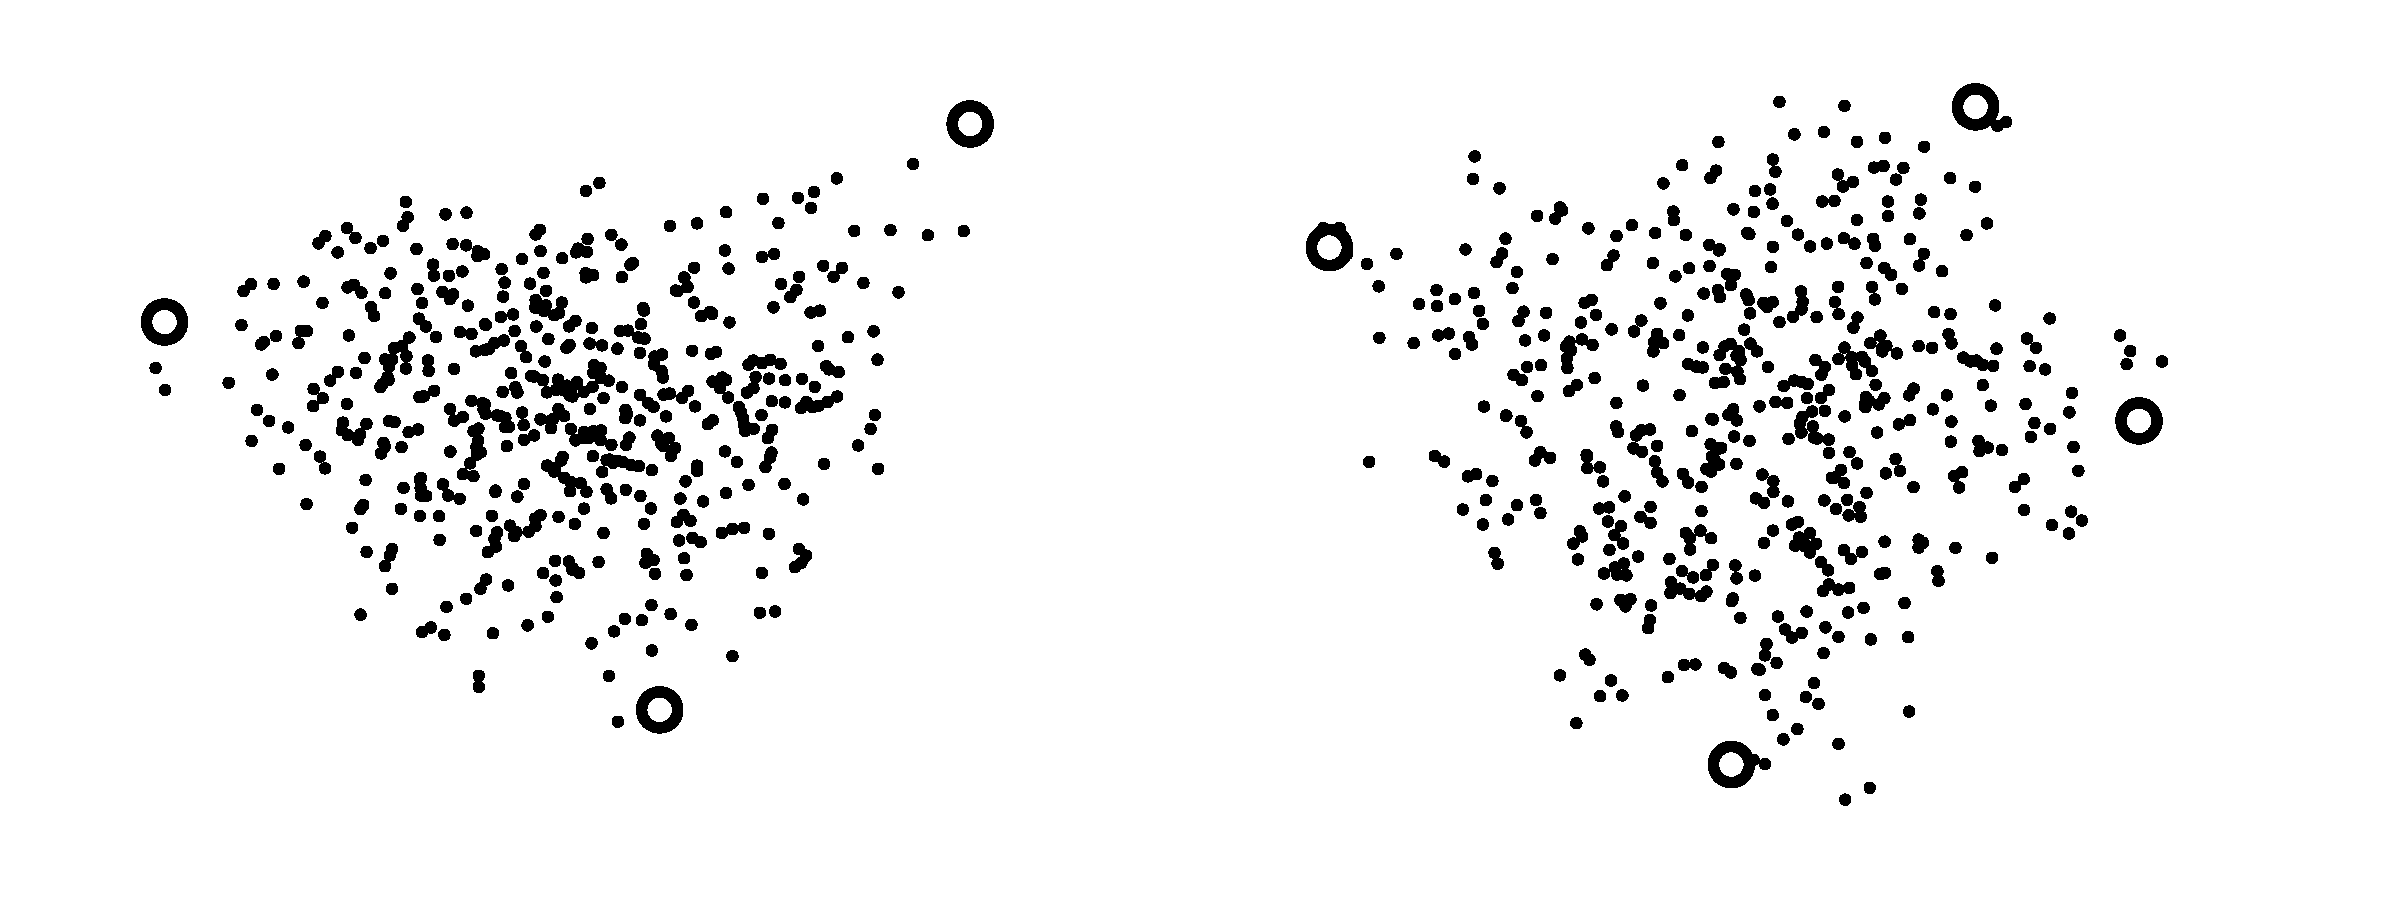
\includegraphics[width=1\linewidth]{figures/AA}
	\caption{\label{fig:AA}Two generic examples of archetypes in multidimensional data. Hollow circles represent the archetypes which are typically located in \textit{corner}-like regions of the data.}
\end{figure}

\subparagraph*{Numerical methods for estimation of archetypes}
Cutler et. al. solved the AA problem using an alternating optimization approach. Starting from a random initialization of $\matr{S}$ the method alternates between finding the best $\matr{C}$ for an $\matr{S}$ and finding the best $\matr{S}$ for a $\matr{C}$, for as necessary until the reduction in $RSS$ is sufficiently small. Each iteration requires solving several convex least squares problems and convergence is slow for many points in high dimensions because the number of points on the convex hull increases exponentially (see Figure \ref{fig:convexHullCurseOfDimensionality}.a. Recent work due to M\o rup and Hansen introduces an effective initialization procedure and a projected gradient approach to solving the AA matrix factorization problem, which however reduces the computation time by limiting the number of points on the convex hull that can constitute solutions to the optimization problem\mcite{morup2012archetypal}. It furthermore allows the analyst to compute archetypes with \texit{slack} such that they may fall outside of the convex hull, diminishing the problem illustrated in Figure \ref{fig:convexHullCurseOfDimensionality}.b.


\subparagraph*{Available implementations}
A number of implementations of AA are available across different software languages. Morup et. al. gives an implementation of their proposed projected gradient version of AA\mcite{morup2012archetypal} which has furthermore been translated into a Python package, by this author, available on the Python Package Index (PyPI). The Python package PyMF also gives an implementation of the, however, slightly slower alternating optimization version of AA\mcite{pymf}. Finally, there is an implementation in R that also uses the traditional approach\mcite{eugster2009spider}.

\subparagraph*{Alternative methods}
As far as the ParTI principle is concerned the only requirements of archetypes is that they constitute the geometrical corners of the dataset. As such other methods for computing archetypes are just as valid as AA. Four alternative methods estimate archetypes using minimal volume simplex and spectral unmixing methods using different approaches\mcite{bioucas2009variable, li2008minimum, chan2009convex, bioucas2009variable}. It is, however, not within the scope of this thesis to further discuss any of these methods.

\newpage
\setcounter{figure}{0}
\thispagestyle{plain}


% Dataset
% -------
\section{Datasets \label{sec:datasets}}
Four different datasources are used in this study. Each one contains multiple datasets and are used for slightly different purposes. Table \ref{tab:dataSourceOverview} gives an overview of which datatypes each source provides. They all have in common that they provide Big Five data for a large number of survey responders which is useful for the analysis presented in Section \ref{subsec:consensusArchetypes}. Appendix \ref{app:BFdist} gives a comparative overview of all Big Five datasets.

\newcommand{\OK}{\ding{51}}%
\begin{table}[!ht]
	\centering
	\begin{tabular}{r|ccccc|c}
	{}				& Big Five	& Facets	& Values	& Attributes	& Behavior 	& 	N (appr.)	\\ \cline{1-7}
	SensibleDTU		& \OK		& -			& -			& -				& \OK		& 	$1\mathrm{E}3$		\\
	myPers.-project	& \OK		& -			& \OK		& -				& 			& 	$2.5\mathrm{E}6$		\\
	SAPA-project	& \OK\OK\OK	& \OK		& 			& \OK			& 			& 	$3-78\mathrm{E}3$		\\
	MIDUS			& \OK\OK\OK	& -			& -			& -				& 			& 	$3-7\mathrm{E}3$
	\end{tabular}
	\caption{\label{tab:dataSourceOverview} Overview of the types of data contained in each used dataset. '\OK' symbolizes that the source contains a given type, and if there are multiple it means that the source contains multiple sets of the type. '-' symbolizes that the type is contained in the datasource but is not used in the analysis.}
\end{table}

	% Sensible DTU
	\subsection{Sensible DTU \label{subsec:sensibleDTU}}
	Sensible DTU was an experiment conducted as part of the ongoing interdisciplinary research project \textit{Social Fabric} at Copenhagen University (UCPH) and DTU Compute of The Technical University of Denmark (DTU), which ran from September 2013 to January 2015 (2.5 years). In the experiment, 863 undergraduate students at DTU gave informed consent to participate. Participants were predominantly male (78.8\%), of average age 21.7 (SD 2.8) years, distributed across all study lines, and were primarily 1st year students (59.2\%) and 2nd year students (30.2\%). Remaining students were either 3rd year students or students for which a year was not reported. Participants were provided a NEXUS smartphone for personal use, which was reprogrammed to continuously collect social behavioral data through multiple channels\mcite{sensibleDTUdocumentation, stopczynski2014a}. Tab. \ref{tab:datatypes} gives an overview of which social behavioral data were collected.

\begin{table}[b!]
	\centering
	\bgroup
	\def\arraystretch{1.2}
	\begin{tabular}{R{4.0cm}|C{2.5cm}C{3cm}}
		\toprule
		\textit{Datatype} & \textit{Sample period} & \textit{Used in this study}\\
		\hline\hline
		GPS-location         &  15 minutes &  \textbf{Yes} \\
		WiFi-scans           &  10 minutes &  No \\
		Bluetooth-scans      &  5 minutes  &  \textbf{Yes} \\
		Phone calls          &  -          &  \textbf{Yes} \\
		Text messages        &  -          &  \textbf{Yes} \\
		Facebook data        &  -          &  No \\
		Screen on/off events &  -          &  \textbf{Yes} \\
		\bottomrule
	\end{tabular}
	\egroup
	\caption{\label{tab:datatypes}Overview of the datatypes which were collected through the administered smartphones, and which are used in this study. Niether channel provides written or spoken content. The Facebook channel includes friends, groups, interests, likes, political orientation, religion and more.}
\end{table}

The experiment saw its largest volume of activity in the spring of 2014, where 526 students were actively using the provided smartphone as their primary device (active on more than 75\% of days through the period, see Fig. \ref{fig:data_activity}).

\begin{figure}[h!]
	\centering
	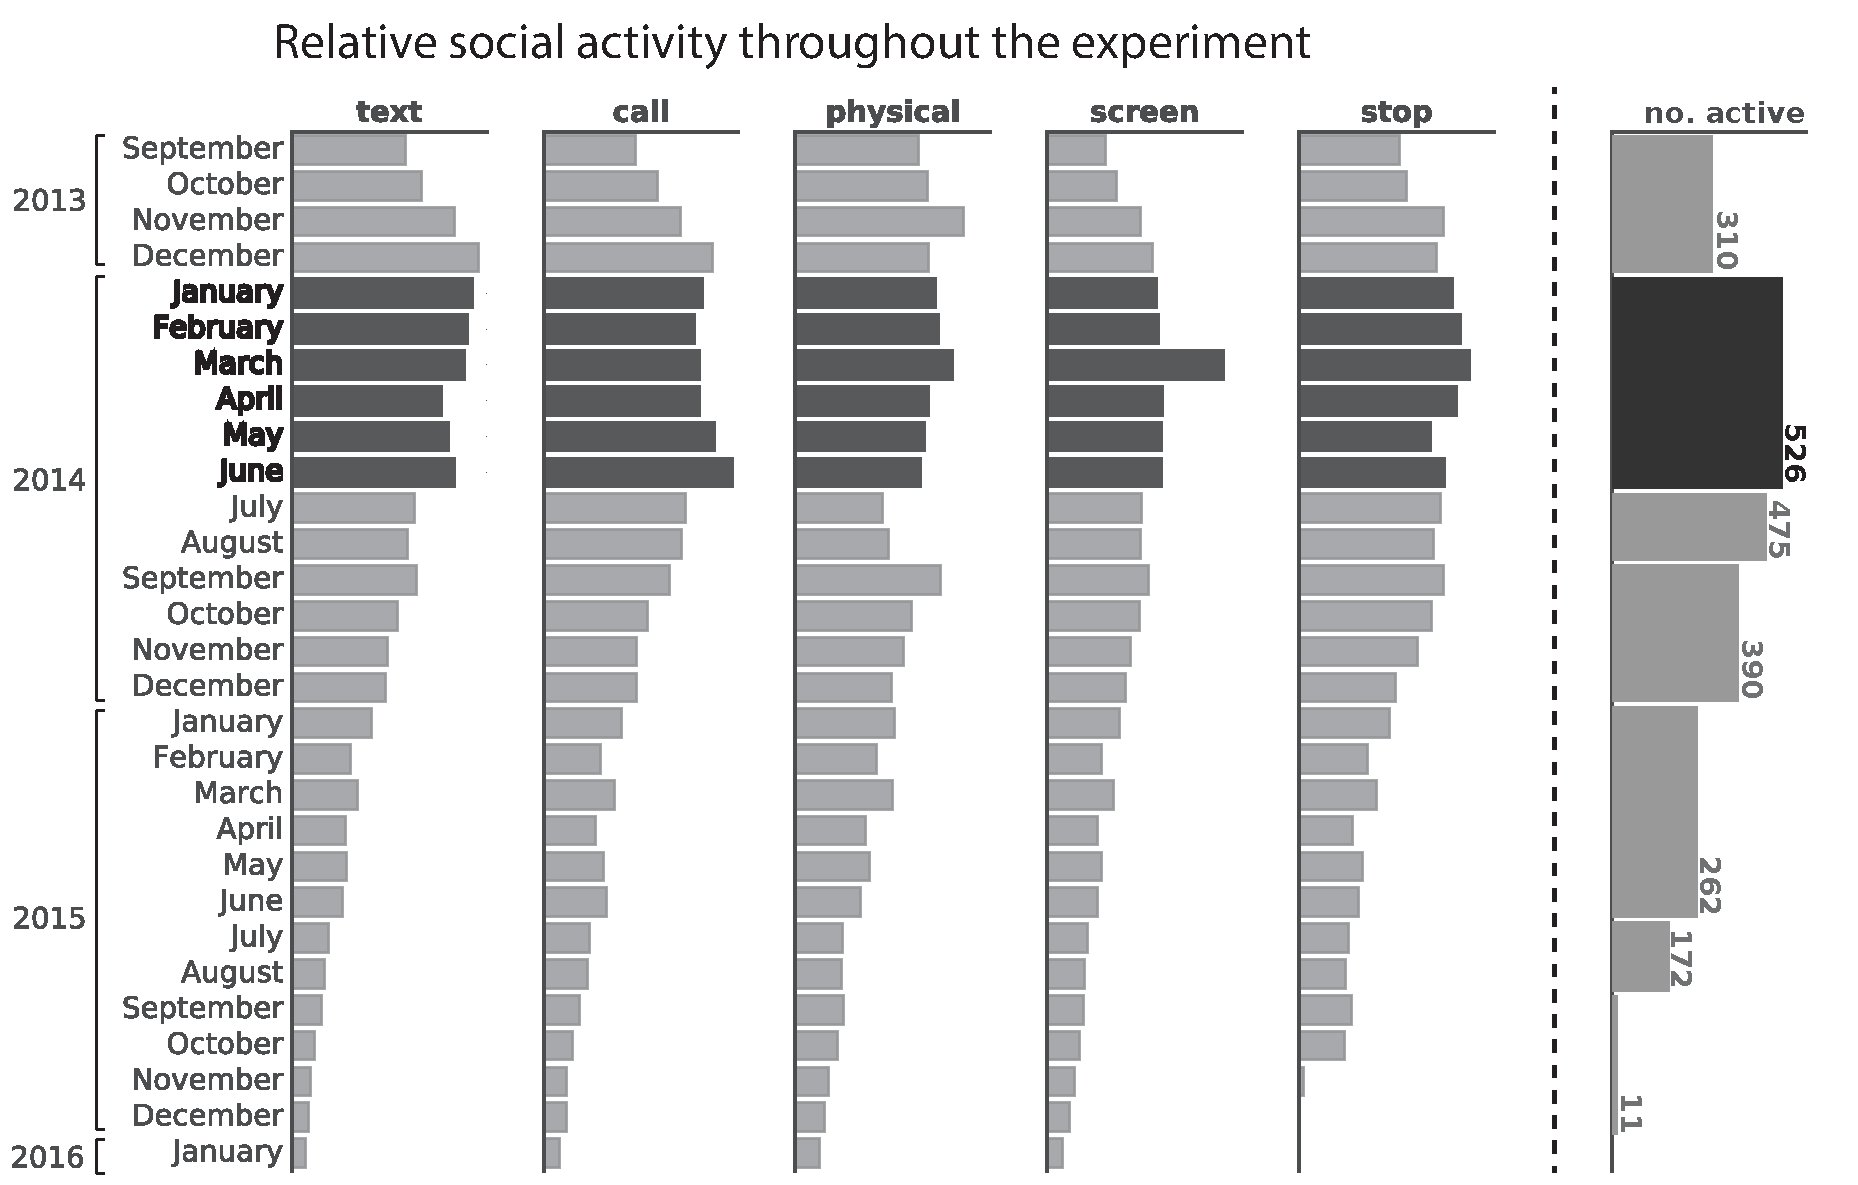
\includegraphics[width=0.8\linewidth]{figures/data_activity}
	\caption{\label{fig:data_activity}An overview of the amount of activity tracked in the respective months of the experiment. The months marked in bold represent those with which the data used in this study is associated. The far right bar plot show the number of students in each semester and summer holiday, which are active on more than 75\% of days through the period.}
\end{figure}

As described in Sec. \ref{subsubsec:behaviorAndPersonality}, behavioral inconsistency sets a limit for the level of mutual information, or correlation, there may be found between a personality trait obtained through a questionnaire, and a specific type of behavior. To mitigate such influence, data originating only from school weeks in the spring semester of 2014 is selected for analysis, based on the assumption that this provides the highest degree of self-similarity in the data. Similar subsets, e.g. from exam periods or holiday weeks, could also have been chosen, but would contain less data since these are narrower spans of time.

Before receiving the phone, participants were required to fill out a baseline questionnaire. It included the Big Five (BF) questionnaire which was used in this study to obtain BF profiles for each subject (see Sec. \ref{subsubsec:dimensionsOfPersonality}). The BF questionnaire was filled out for each participant no later than december 20th of 2013\mcite{sensibleDTUdocumentation}. The notion raised in Section \ref{subsubsec:behaviorAndPersonality} that behavior and personality are not constants provides a compelling argument that they should be measured as close in time as possible, which gives another reason for choosing to use only behavioral data from the spring semester of 2014.
%Fig. \ref{fig:big_five_violin_plots} shows violin plots for the different Big Five traits in the dataset.

% \begin{figure}
% 	\centering
% 	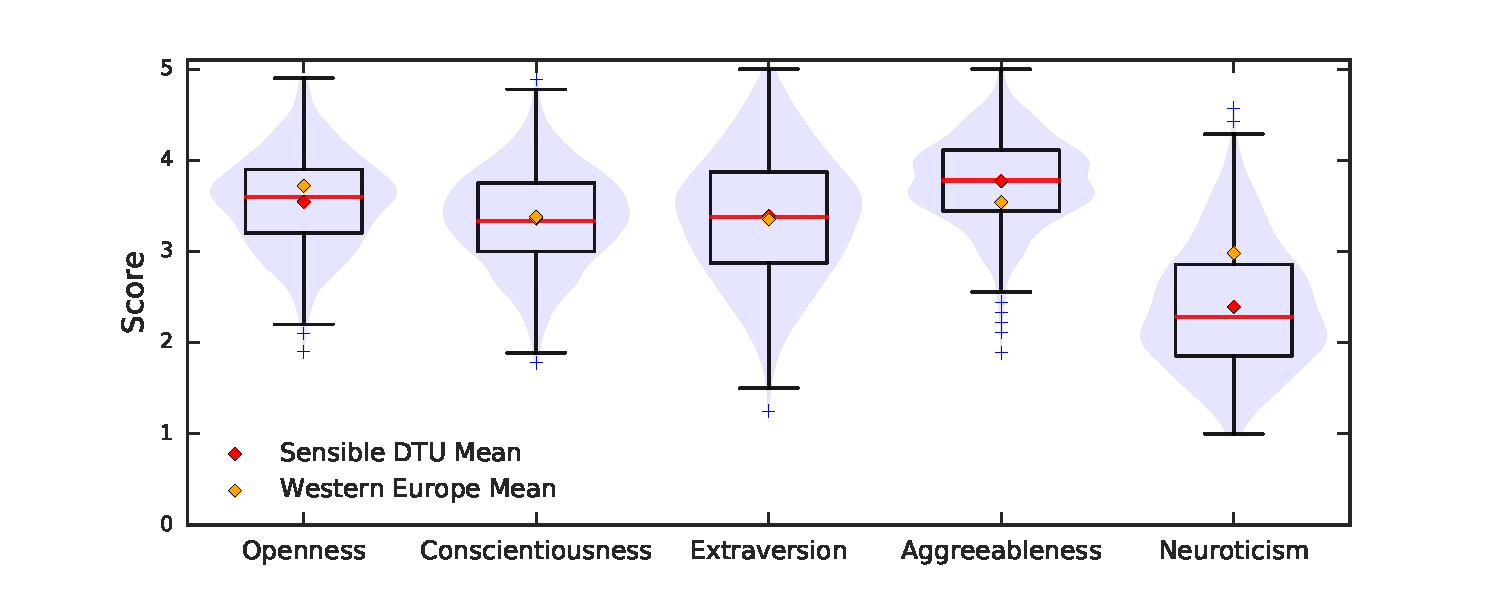
\includegraphics[width=0.8\linewidth]{figures/big_five_violin_plots}
% 	\caption{\label{fig:big_five_violin_plots}Violin plots of Big Five personality traits in the Sensible DTU data. Summary statistics of the format \texttt{mean} (\texttt{SD}) are: openness 3.58 (0.52); conscientiousness 3.44 (0.51); extraversion 3.15 (0.53); agreeablenes 3.64 (0.51); neuroticism 2.59 (0.65). Red dots represent mean values in this study and orange diamonds are mean in Western Europe (mixed population)\cite{schmitt2007geographic}.}
% \end{figure}

Researchers in the Social Fabric project also has access to administrative data such birth year, courses, drop-out and most notably grades, none of which, however, were used in this study.

\subparagraph*{Privacy and data access} Given the sensitive information contained, or easily extracted, from this data despite all reference to personal identity having been removed, strict access rules to the data are imposed. Researchers are obliged to sign a non-disclosure aggreement (NDA) and raw data is not to be contained on private of public machines outside of the EU. Data is accessed in JSON format through the Data Viewer API at \texttt{sensible.dtu.dk/apps/data\_viewer} with a valid research token, or through a virtual IPython Notebook environment hosted at \texttt{raw.sensible.dtu.dk}, where data is served as Numpy MaskedArray type for efficiency which easily converts to Pandas DataFrame type, Numpy 2D array or similar matrix-like types (see Sec. \ref{subsec:behavioralDataPreprocessing} for technical reference). Researchers working outside of the EU are restricted to work with the data remotely through the virtual IPython Notebook environment, which is, conveniently, also the faster alternative.

	% myPersonality
	\subsection{myPersonality \label{subsec:facebook}}
	The myPersonality research project maintained a Facebook application through which users could answer various personality questionnaires and donate personal data from their profiles\mcite{kosinski2015facebook}. It reached great popularity because it allowed users to compare results with friends and even fill out personality questionnaires for others. From 2007 to 2012 the research project managed to collect questionnaire responses from nearly 7.5 million Facebook users. 900.000 users retook the questionnaire providing longitudinal data, 300.000 provided friend ratings enabling self-report accuracy assessment and 40\% gave full access to private profile information.

In the current study, access to approximately 2.5 million BF profiles and 9000 'Basic Human Values' (BHV) questionnaire responses were provided. BHVs stem from the Theory of Basic Human Values due to Shalom Schwartz\mcite{schwartz1992universals, schwartz2012overview}, which juxtapose the 10 fundamental values: \textit{benevolence}, \textit{tradition}, \textit{conformity}, \textit{security}, \textit{power}, \textit{achievement}, \textit{hedonism}, \textit{stimulation}, \textit{self-direction}, \textit{universalism}. An overview of value/facet-relationships of their position relative to each other is given in Appendix \ref{app:theoryOfBasicHumanValues}.

	% MIDUS
	\subsection{Midlife Development in the U.S \label{subsec:MIDUS}}
	Midlife Development in the U.S (MIDUS) was a longitudinal telephone/email survey study conducted in three waves in 1995, 2004/06 and 2013\mcite{brim2004midus}. Its goal was to create a dataset which could be analyzed to understand how various life variables affect each other. It successfully collected repeated questionnaire responses for 3294 randomly selected Americans, which, among many other metrics, included personality profiles measured with the BFM. For the BF items in the survey participants rated how well different words described them on a four tick scale.
In this study, BF datasets from each of the waves are used. MIDUS 1 has 6261 valid datapoints, MIDUS 2 has 3971 and MIDUS 3 has 2715. Importantly the MIDUS 2 and MIDUS 3 datapoints are measurements of participants who are also measured on in the previous years. For the intended purpose this is not thought to have any damaging influence on the results, but is still important to keep in mind. Considering Appendix \ref{app:BFdist} is can furthermore be seen that the \CON, \EXT, and \AGR traits do not distribute normally, but seem highly shifted towards higher values. This may be due to bias in the collection method which relied on an interviewer to collect the responses over telephone, or possible an artifact of the inventory used.

	% SAPA
	\subsection{SAPA-Project \label{subsec:SAPA}}
	SAPA stands for 'Synthetic Aperture Personality Assessment' which is a survey collection method that feeds the respondent with semi-random questions from a large pool of questionnaire items from a variety of inventories, until the respondent stops answering. This creates a sparse dataset of response values, but for a large number of participants, covariance matrices between questionnaire items across people with different attributes (e.g. country/gender) can be computed to infer differences between groups.
The SAPA-Project is an effort by computational psychologist David Condon, which works as a web application allowing Internet users to take a personality test and get insights about themselves\mcite{condon2014}. In turn it is also a tools for researchers to gather personality data. Participants disclose various personal demographic information and respond to questions from three BF inventories: IPIP100, IPIP-NEO and SPI. The first two are internationally recognized pools of questionnaire items\mcite{donnellan2006mini}, while the last one is a product if Condon's thesis\mcite{condon2014}. Each one derives the BFTs using slightly different approached but largely produce the same factors. Using only responders who answered at least four items for each trait, the IPIP100 inventory has 77,685 valid datapoints, the SPI inventory has 2928 valid datapoints and the IPIP-NEO has 37,554 valid datapoints. 100\% of valid responders to the SPI inventory are also valid responders to the IPIP-NEO inventory and 47\% of valid responders to the IPIP-NEO inventory are also valid responders to the IPIP100 inventory.

An excerpt of the SAPA data is freely avaiable through the Harvard Dataverse at \url{https://goo.gl/vrX83G}.



\newpage
\setcounter{figure}{0}
\thispagestyle{plain}


% Results
% -------
\section{Analysis and Results\label{sec:results}}
The research objective is to find fundamental personality archetypes and understand which behavioral strategies they correspond to in terms of the their personality facets, demographic attributes, values and correlated behaviors.
As stated in the introduction this thesis documents the first efforts in an ongoing research project, and as such the above goal is bold and will not be exhaustively satisfied.
The results do however offer clues towards \textit{which} evolutionary behavioral strategies can be inferred from data.

The analysis takes the following trajectory:
Six archetypes are found to emerge consistently across multiple datasets.
For each, values, personality facets, personal attributes and behavior is inferred.
The features of each archetype differ in fundamental ways and provide clues towards strategies for performing life's many tasks.
These are speculated to be: (1) \achiever (power/achievement driven, emotionally stable, unsympathetic), (2) \host (achievement driven, highly social, emotionally unstable), (3) \wildcard (conformist, benevolent, social, emotionally stable), (4) \loyalist (narrow-minded, loyal, orderly), (5) \hippie (unconformed, undutiful, unorganized, unworried, emotionally stable) and (6) \follower (antisocial, depressed, worried, emotionally unstable).
Note that for the sake of clarity these strategy labels are used throughout the analysis before they are given fair justification.

The analysis is separated into parts that each has a single premise.
Each motivates the next and together they discover the strategies.
The first part presents the analysis leading to the discovery of \textit{consensus archetypes}, a relaxed interpretation of an archetype.
The second part investigates the types of personal attributes that are enriched near each consensus archetype, and which stable behavioral indicators correlate with distance from the archetypes.
The third part investigates the predictive power of the consensus archetypes compared to raw BFTs and PCs of BF questionnaire items (QI).
Technical details about the analysis are explained in Section \ref{subsec:methods:analysis}.

	% Consensus Archetypes
	\subsection{Six consensus archetypes emerge across seven datasets \label{subsec:consensusArchetypes}}
	The search for six strategies has two motivations. The first is that, as was shown in Section \ref{subsubsec:ParTIptOne} Figure \ref{fig:convexHullCurseOfDimensionality}, for more than five dimensions most points are in the convex set of points and therefore not inside of the Pareto front, unless the number of points becomes very large. As such, this justifies six as an upper bound.
The lower bound is slightly harder to justify, but an argument can be found in the fact that there are five personality factors.
In Section \ref{subsubsec:dimensionsOfPersonality} the Big Five model was presented and it was explained that the covariance of personality descriptive adjectives applied to subjects within a large enough population across a multitude of studies leads to five significant factors of personality.
The ParTI principle states that objectives (here: strategies) are the $d+1$ vertices of the simplex on which points fall in the $d$-dimensional subspace of greatest variance, and since personality varies strongly along five factors, there should not be less than six fundamental personality strategies.

\textbf{Archetypes are computed for multiple datasets to ensure generality}.
Under the assumption that no questionnaire inventory and sample population can provide enough generality to find the fundamental personality archetypes, the ParTI principle is applied to seven different datasets (see Section \ref{sec:datasets}).
The Sensible DTU BF dataset is left out because the population is deemed to specified to produce general enough archetypes.
For each dataset archetypes are computed as median values over 5000 bootstrapping iterations with sample size 200.
The emerging sets of archetypes (median values) are presented in Figure \ref{fig:medianDistances}. Section \ref{subsec:computingConsensusArchetypes} explains in detail how the archetypes are computed.

\begin{figure}
	\centering
	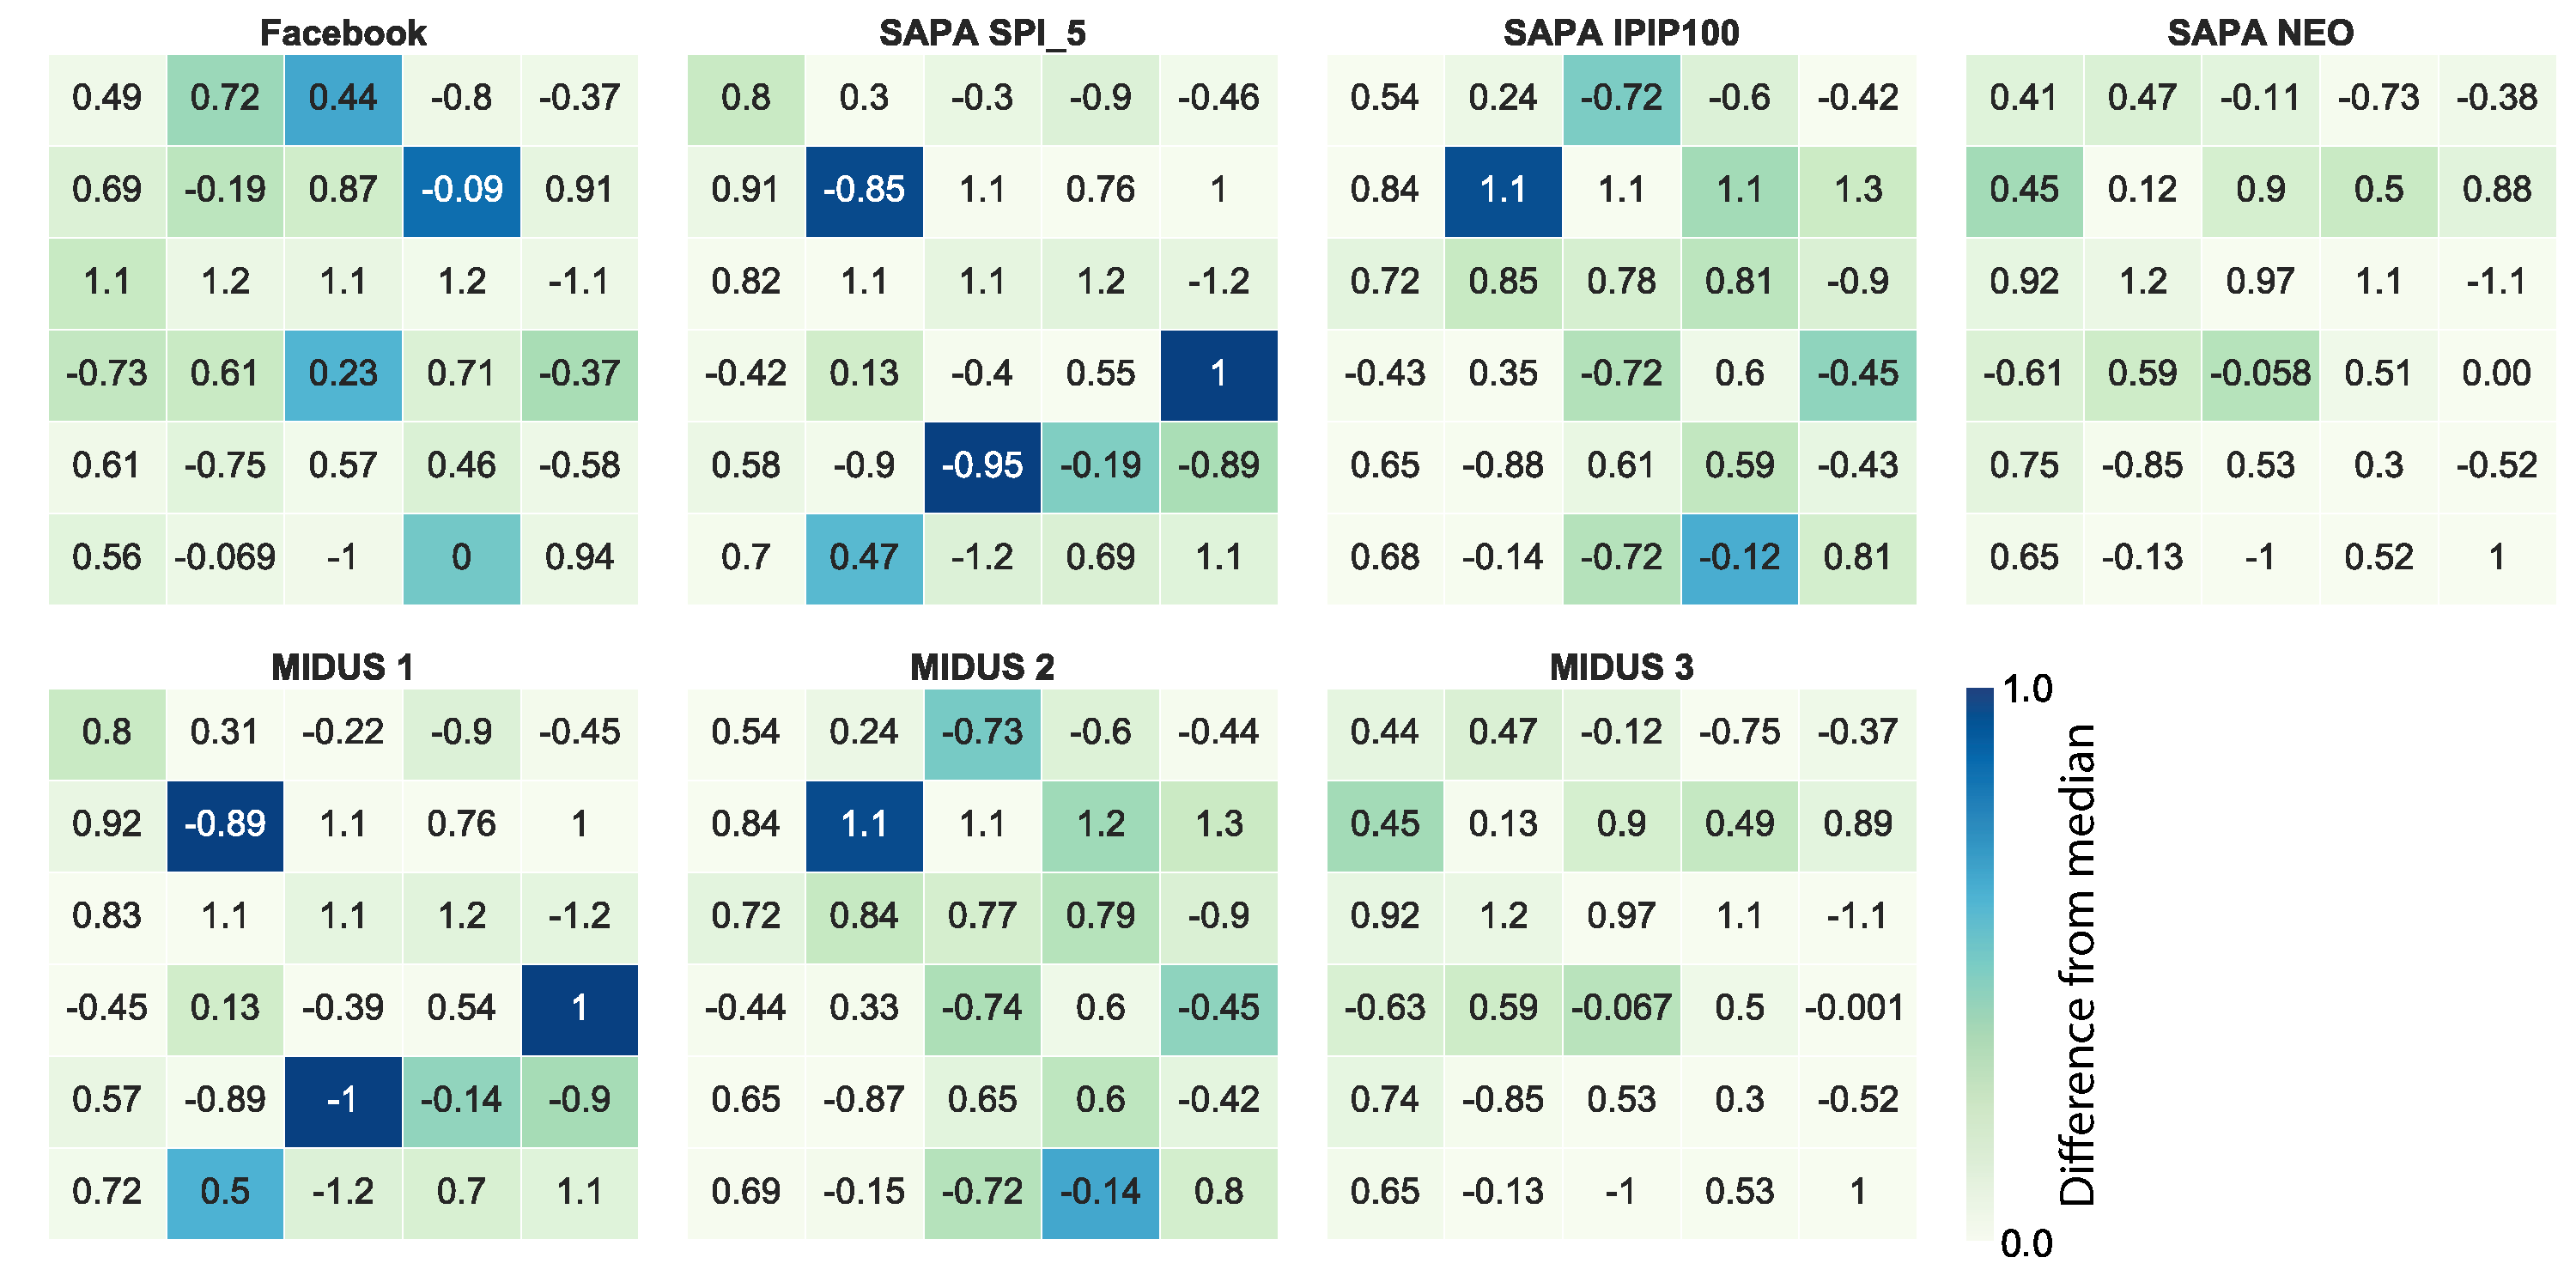
\includegraphics[width=\textwidth]{figures/medianDistances}
	\caption{\label{fig:medianDistances} Archetypes emerging from each dataset.
	Color map scales with archetype trait distances from archetype trait median across all datasets.
	Annotated values are rows of archetypes and BFTs as columns ordered by O, C, E, A and N.}
\end{figure}

\textbf{Archetype deviations across datsets reveal \textit{consensus archetypes}}. 
Figure \ref{fig:medianDistances} shows that roughly the same archetypes emerge from the different datasets.
However, certain archetype traits are far from the median.
Since these are large datasets from mixed populations it is not believed that any one produces archetypes that are severely different due to noise.
Rather the differences are believed more likely to arise due to characteristics relating to the population and the questionnaire inventory.
To investigate the severity of the differences a $6 \times 5$ array of SDs across the datasets (stacked in depth and calculated along 2nd axis, see Section \ref{subsec:computingConsensusArchetypes}) is computed, and shown in Figure \ref{fig:varianceThreshold}.a.
Due to the observation that some archetype traits appear to have much higher SD than others a \textit{consensus threshold} of maximum SD, $\lambda$, is set for a significance level $\alpha = 0.05$.
To find the threshold, an SD value array is computed multiple times for shuffled archetype traits (columns shuffled independently).
All resulting SDs are then arranged in a list and sorted to ascending order, and the largest value of the lower 5th percentile is chosen as the threshold.
This method results in $\lambda = 0.22$.
The distribution of SDs and shuffled archetype SDs are visualized in Figure \ref{fig:varianceThreshold}.b.
Clearly there is a group of archetype traits with low SD and one with high SD.
$\lambda$ gives rise to a mask that decides which archetype traits are in consensus and which are not.
Applying the mask to the median archetypes across all datasets reveals the \textit{consensus archetypes} (CA) presented in Figure \ref{fig:consensusArchetypes}.a.
For consistency the CAs are here named according to their later speculated strategies.\\

\begin{figure}
	\centering
	\begin{minipage}[l]{0.45\textwidth}
		\centering
		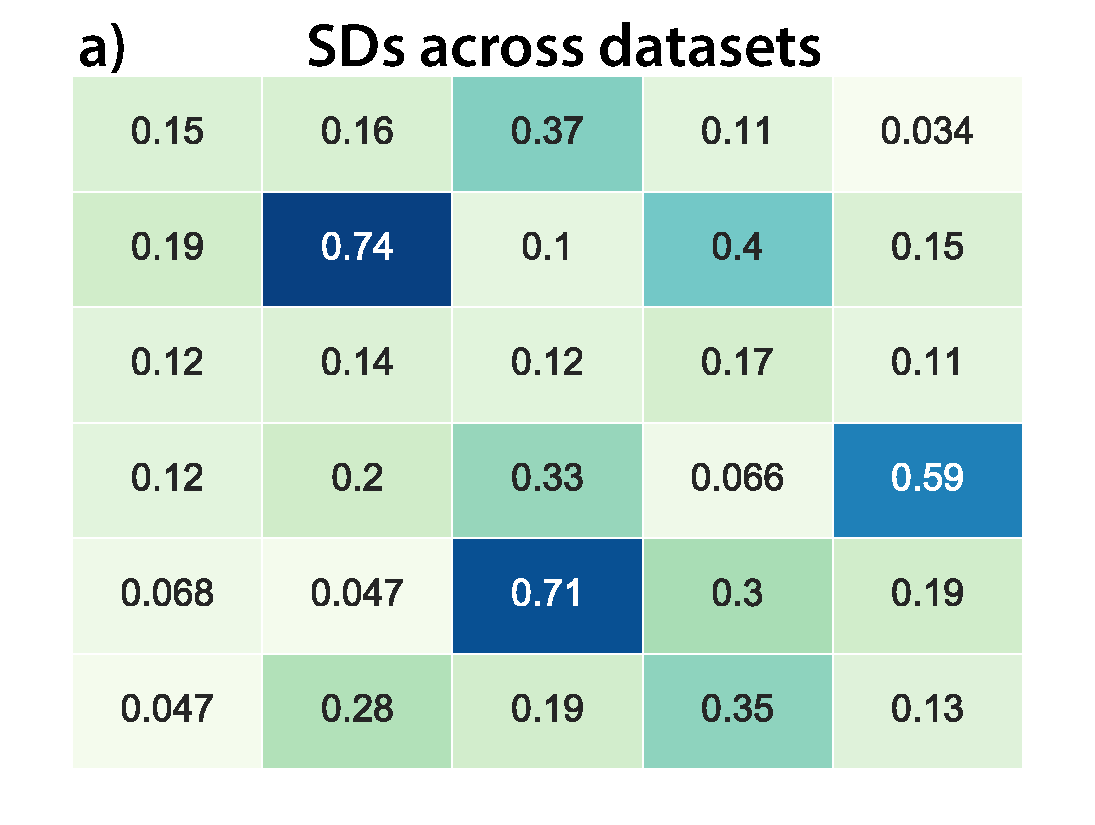
\includegraphics[width=\textwidth]{figures/stdsAcrossDatasets}
	\end{minipage}
	\begin{minipage}[r]{0.52\textwidth}
		\centering
		\vspace{0.2cm}
		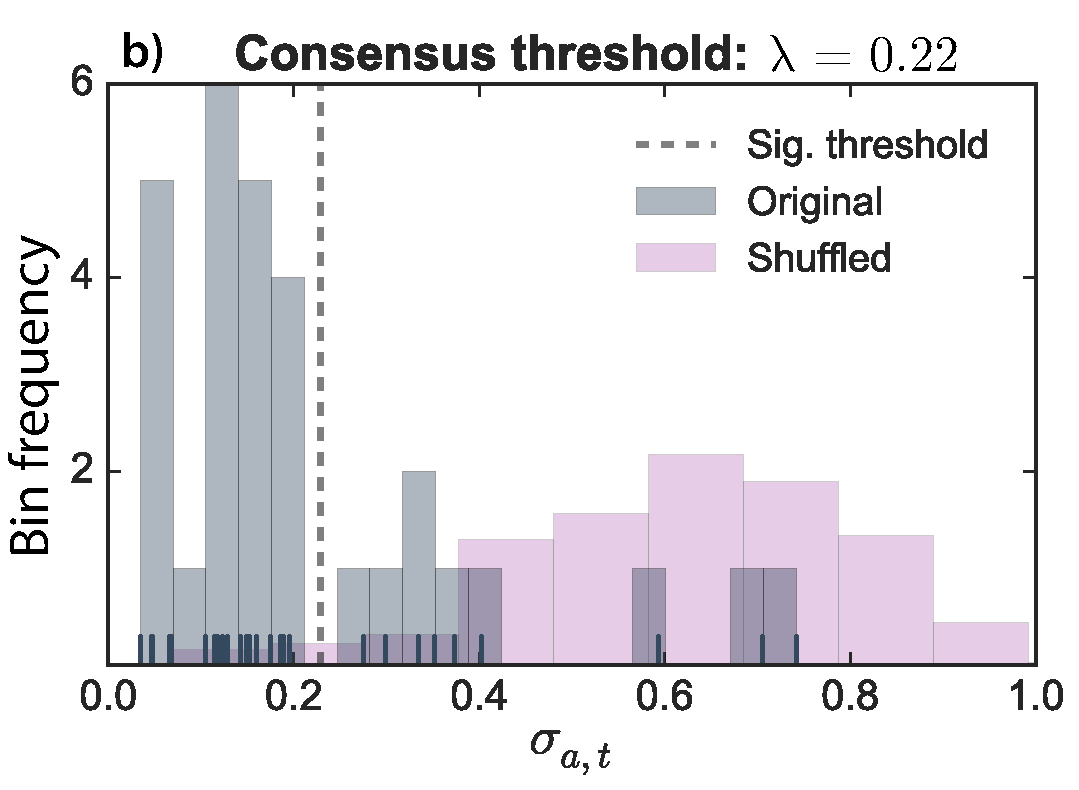
\includegraphics[width=\textwidth]{figures/varianceThreshold}
	\end{minipage}
	\vspace{-0.25cm}
	\caption{\label{fig:varianceThreshold} \textbf{a)} SD values for archetype traits across datasets.
	It is observed that some vary greatly while others are very stable. \textbf{b)} A consensus threshold $\lambda$ emerges at 0.22, which gives rise to $p$-values less than 0.05 for all archetype traits below the consensus threshold.
	The purple histogram shows the normalized distribution of SDs for shuffled archetype traits.
	The blue histogram shows the normalized distribution of SDs of the actual archetypes, where the rug shows distribution of individual SDs.}
\end{figure}

\begin{figure}
	\centering
	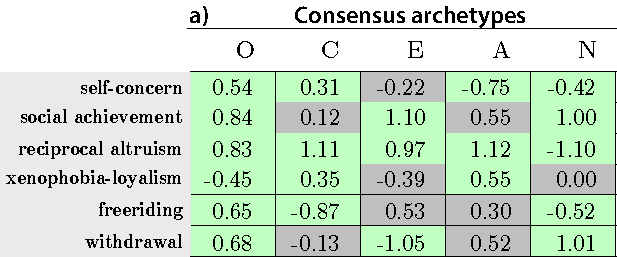
\includegraphics[width=0.7\textwidth]{figures/consensusArchetypes}
	\hspace{0.2cm}
	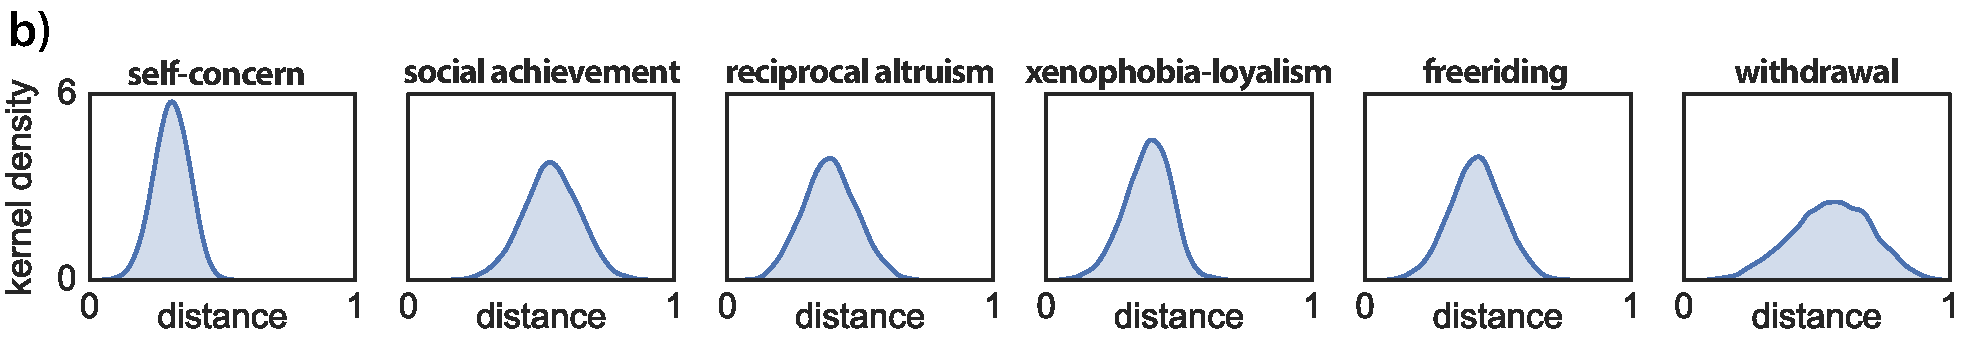
\includegraphics[width=\textwidth]{figures/archetypeDistanceDistributions}
	\caption{\label{fig:consensusArchetypes} \textbf{a)} \textbf{Main result of Section \ref{subsec:consensusArchetypes}}.
	Consensus archetypes emerge as median archetypes where trait values are colored with respect to the consensus threshold: green signifies consensus and gray signifies above threshold non-consensus, i.e.
	undefined dimensions. \textbf{b)} Distributions of weighted euclidean distances from points in the Facebook dataset to consensus archetypes. Axes are scaled equally.}
\end{figure}

The strategies reveal themselves somewhat from the CA traits.
The \achiever CA is particularly unagreeable, which typically correlates with distrust for others and self-centered motives.
The \follower CA is highly introverted and neurotic which could indicate a \textit{constantly-aware-of-danger} strategy.
In fact, it seems, each archetype is quite distinct from the others.
It is definitely worth taking a short break from reading to get acquainted with the CAs and their individual differences and similarities (see Figure \ref{fig:consensusArchetypes}.a).

A remark on the mathematical implications of CAs should be made.
While there are no strict mathematical definitions of what an archetype is, the discourse so far has implied that it is a \textit{point}.
However, once a consensus mask is applied, certain of the trait values for some of the archetypes are said to be "not in consensus".
What this really means is that when e.g. computing the distance to a CA the weighted euclidean distance must be used, adding zero weight to non-consensus traits while all other weights sum to 1.
As such, if, for an archetype, a single trait is in non-consensus the archetype is effectively a line.
If two traits are in non-consensus it is a plane, if three a volume, if four a hyperplane in five dimensions, etc.
In the following analysis the fact that they are CAs and not just normal archetypes only has importance in terms of computing the distance to them, which is done using the weighted euclidean approach as described.
Therefore CAs will be referred to as \textit{archetypes} unless discussion requires them to be explicitly stated as archetypes in consensus between datasets.

	% Enrichment
	\subsection{Enrichment and correlation reveal distinct strategies\label{subsec:enrichment}}
	From Figure \ref{fig:consensusArchetypes}.a it is observed that some archetypes share very similar trait values.
Comparing e.g. the \host and \follower archetypes they only differ on the \EXT trait.
Does this mean that the two may correspond to the same behavioral strategy? No.
In the following the differences between archetypes are investigated by studying how facets, values, demographic attributes and behaviors are enriched/depleted\footnote{Herinafter just \textit{enriched} to simplify the language.} for- or correlate with distance from the archetypes.
Enrichment analysis is used because it provides an intuitive way of interpreting whether a variable is influenced by distance from an archetype, and correlation analysis is used for behavior where there are not enough datapoints to provide statistically significant results using enrichment analysis (see Section \ref{subsubsec:ParTIptTwo}).
It is important to stress, however, that either of these approaches inform only about statistical \textit{trends} and not absolute differences.
For example, as was stated in Section \ref{subsubsec:behaviorAndPersonality} there is a limit to how well personality and behavior can correlate, empirically fixed around 0.3.
And while the same rule may not necessarily apply for demographic attributes, values and particularly not facets (for reasons explained later), it still raises the important notion that no relationship between \textit{anything} and personality is absolute, because after all (as was raised as critism in Section \ref{subsubsec:behaviorAndPersonality}) the best available method can only explain 56\% of personality variance.
The results presented in the following are therefore only \textit{indicative} and their implications are strictly useful for supporting claims that strategies exist and suggesting what those might then be.
Since the analysis yields many results, this section presents them in summary form.
The full collection of results is presented in Appendices \ref{app:questionnaireEnrichmentTable}-\ref{app:behaviorCorrelationTable}.

% \textbf{Facets and values reveal differences between archetypes}.
% Figure 
% Appendix \ref{app:questionnaireEnrichmentTable} and \ref{app:valuesEnrichmentTable} present all significant enrichments of QIs from the SPI inventory and BHVs, respectively, where rows have been permuted to illustrate for which archetypes maximum enrichment occurs.
% It is noted from Figure \ref{fig:firstEnrichmentsQuestionnaireValues} that there are stronger enrichments for QIs than for BHVs.
% While care has been taken to avoid direct circular enrichment, it appears from the strong QI enrichments that it still occurs implicitly.
% The importance of this analysis is therefore not to highlight how strong the enrichments are, but rather how strong they are relative to each other.
% The combinations of QIs that are enriched for each archetype is not trivial and provides insight about facets.
% For example, when considering enrichment slopes in Appendix \ref{app:questionnaireEnrichmentTable} the \achiever archetype who has above average \OPE achieves that score not by having medium/high values for each QI but by consistently being low in items related to the appreciation for art, creativity and reflection, while being higher on items that relate to understanding things quickly, solving complex problems and knowing the answer to many questions.
% Both classes of facets relate to openness and intelligence, but are not necessarily correlated.

% \textbf{Demographic attribute enrichments indicate niches in society}.
% Categorical demographic variables are studied for enrichment near archetypes.
% Table \ref{tab:attributesTable} shows the most significant demographic attribute enrichments for each archetype.
% It appears that each fulfills a distinct niche in society.
% For the \achiever and \follower archetypes it is observed that enriched disciplines don't involve working with people, which is the opposite for the \host, \wildcard and \loyalist archetypes.
% Curiously, the same two groups also differ in their relationship status, indicating that one strategizes to rely on people while the other does not.
% All archetypes except for \host and \wildcard are enriched for unemployment, where \loyalist and \hippie archetypes are younger and students, and \follower is enriched for retirement which partially explains the unemployment trend.
% The \achiever archetype is, however, young as evidenced by the depletion of age and 'retired' job status, in which case the enrichment of unemployment could point to self-employment of various types.
% The 'smoking' and 'exercise' attributes might not say much about societal niche, but are interesting in themselves and when viewed together.
% The \wildcard archetype exercises and doesn't smoke, the \hippie archetypes smokes but doesn't exercise and the \host archetype both smokes and exercises.
% Smoking and exercise is somewhat contradictory, so why would anyone do both? The \host archetype is enriched for stimulation and hedonism which partially explains this observation, but it also indicates an ability to hold contradictory beliefs simultaneously, which is undoubtedly a useful feature for individuals whose behavioral strategy is to use social engagement to advance in hierarchies.



% Due to the age differences between the archetypes, age-dependent demographic variables such as education level and marital status are not used.


% \textbf{We can now paint a picture of the strategies}
% REWRITE TITLE TO PREMISE FORM.
% There are very clear differences between the archetypes just from the QIs and BHV enrichments.
% The \achiever archetype is an extreme individualist, who is emotionally disconnected and values power and disregards benevolence.
% The \host archetype is a talkative extrovert, highly emotional and values social stimulation and hedonism.
% The \wildcard archetype is conscientious and happy, and strongly values almost every BHV (except hedonism, self-direction and power), and in particular benevolence and conformity.
% The \loyalist archetype values tradition and conformity and is uninterested in abstract ideas and art.
% The \hippie archetype is carefree and messy, values hedonism and stimulation and cares little about security and achievement.
% Finally the \follower archetype is avoids social interaction, worries a lot and values none of the BHVs, and in particular not social stimulation.

		% Analysis and data
		\subsubsection{Analysis and data \label{subsubsec:analysisAndData}}
		Enrichment methods for continuous and categorical variables, as described in Section \ref{subsubsec:ParTIptTwo}, and Pearson product-moment correlation are applied.
Table \ref{tab:facetsValuesAttributesTable} gives a qualitative summary of all enrichments as they are presented in Appendices \ref{app:questionnaireEnrichmentTable}-\ref{app:behaviorCorrelationTable}.
Figure \ref{fig:firstEnrichmentsQuestionnaireValues} visualizes the strongest enrichments of QIs and BHVs, as well as enrichment of professional disciplines for each archetype, to give the reader an intuition of the method.
Because both enrichment and correlation methods uses \textit{distance} from archetype as the independent variable, negative slopes signify enrichment and positive slope signifies depletion.
Error bars have been omitted because they vanish due to the large sample sized, however SDs are typical in the order of a quarter of the second axis range which is not insignificant to the later interpretation of the enrichments.
All presented enrichments and correlations in Table \ref{tab:facetsValuesAttributesTable} and Figure \ref{fig:firstEnrichmentsQuestionnaireValues} are significant after Bonferroni and Benjamin-Hochberg corrections, respectively, for a significance level of 0.05.

\begin{figure}[!ht]
	\centering
	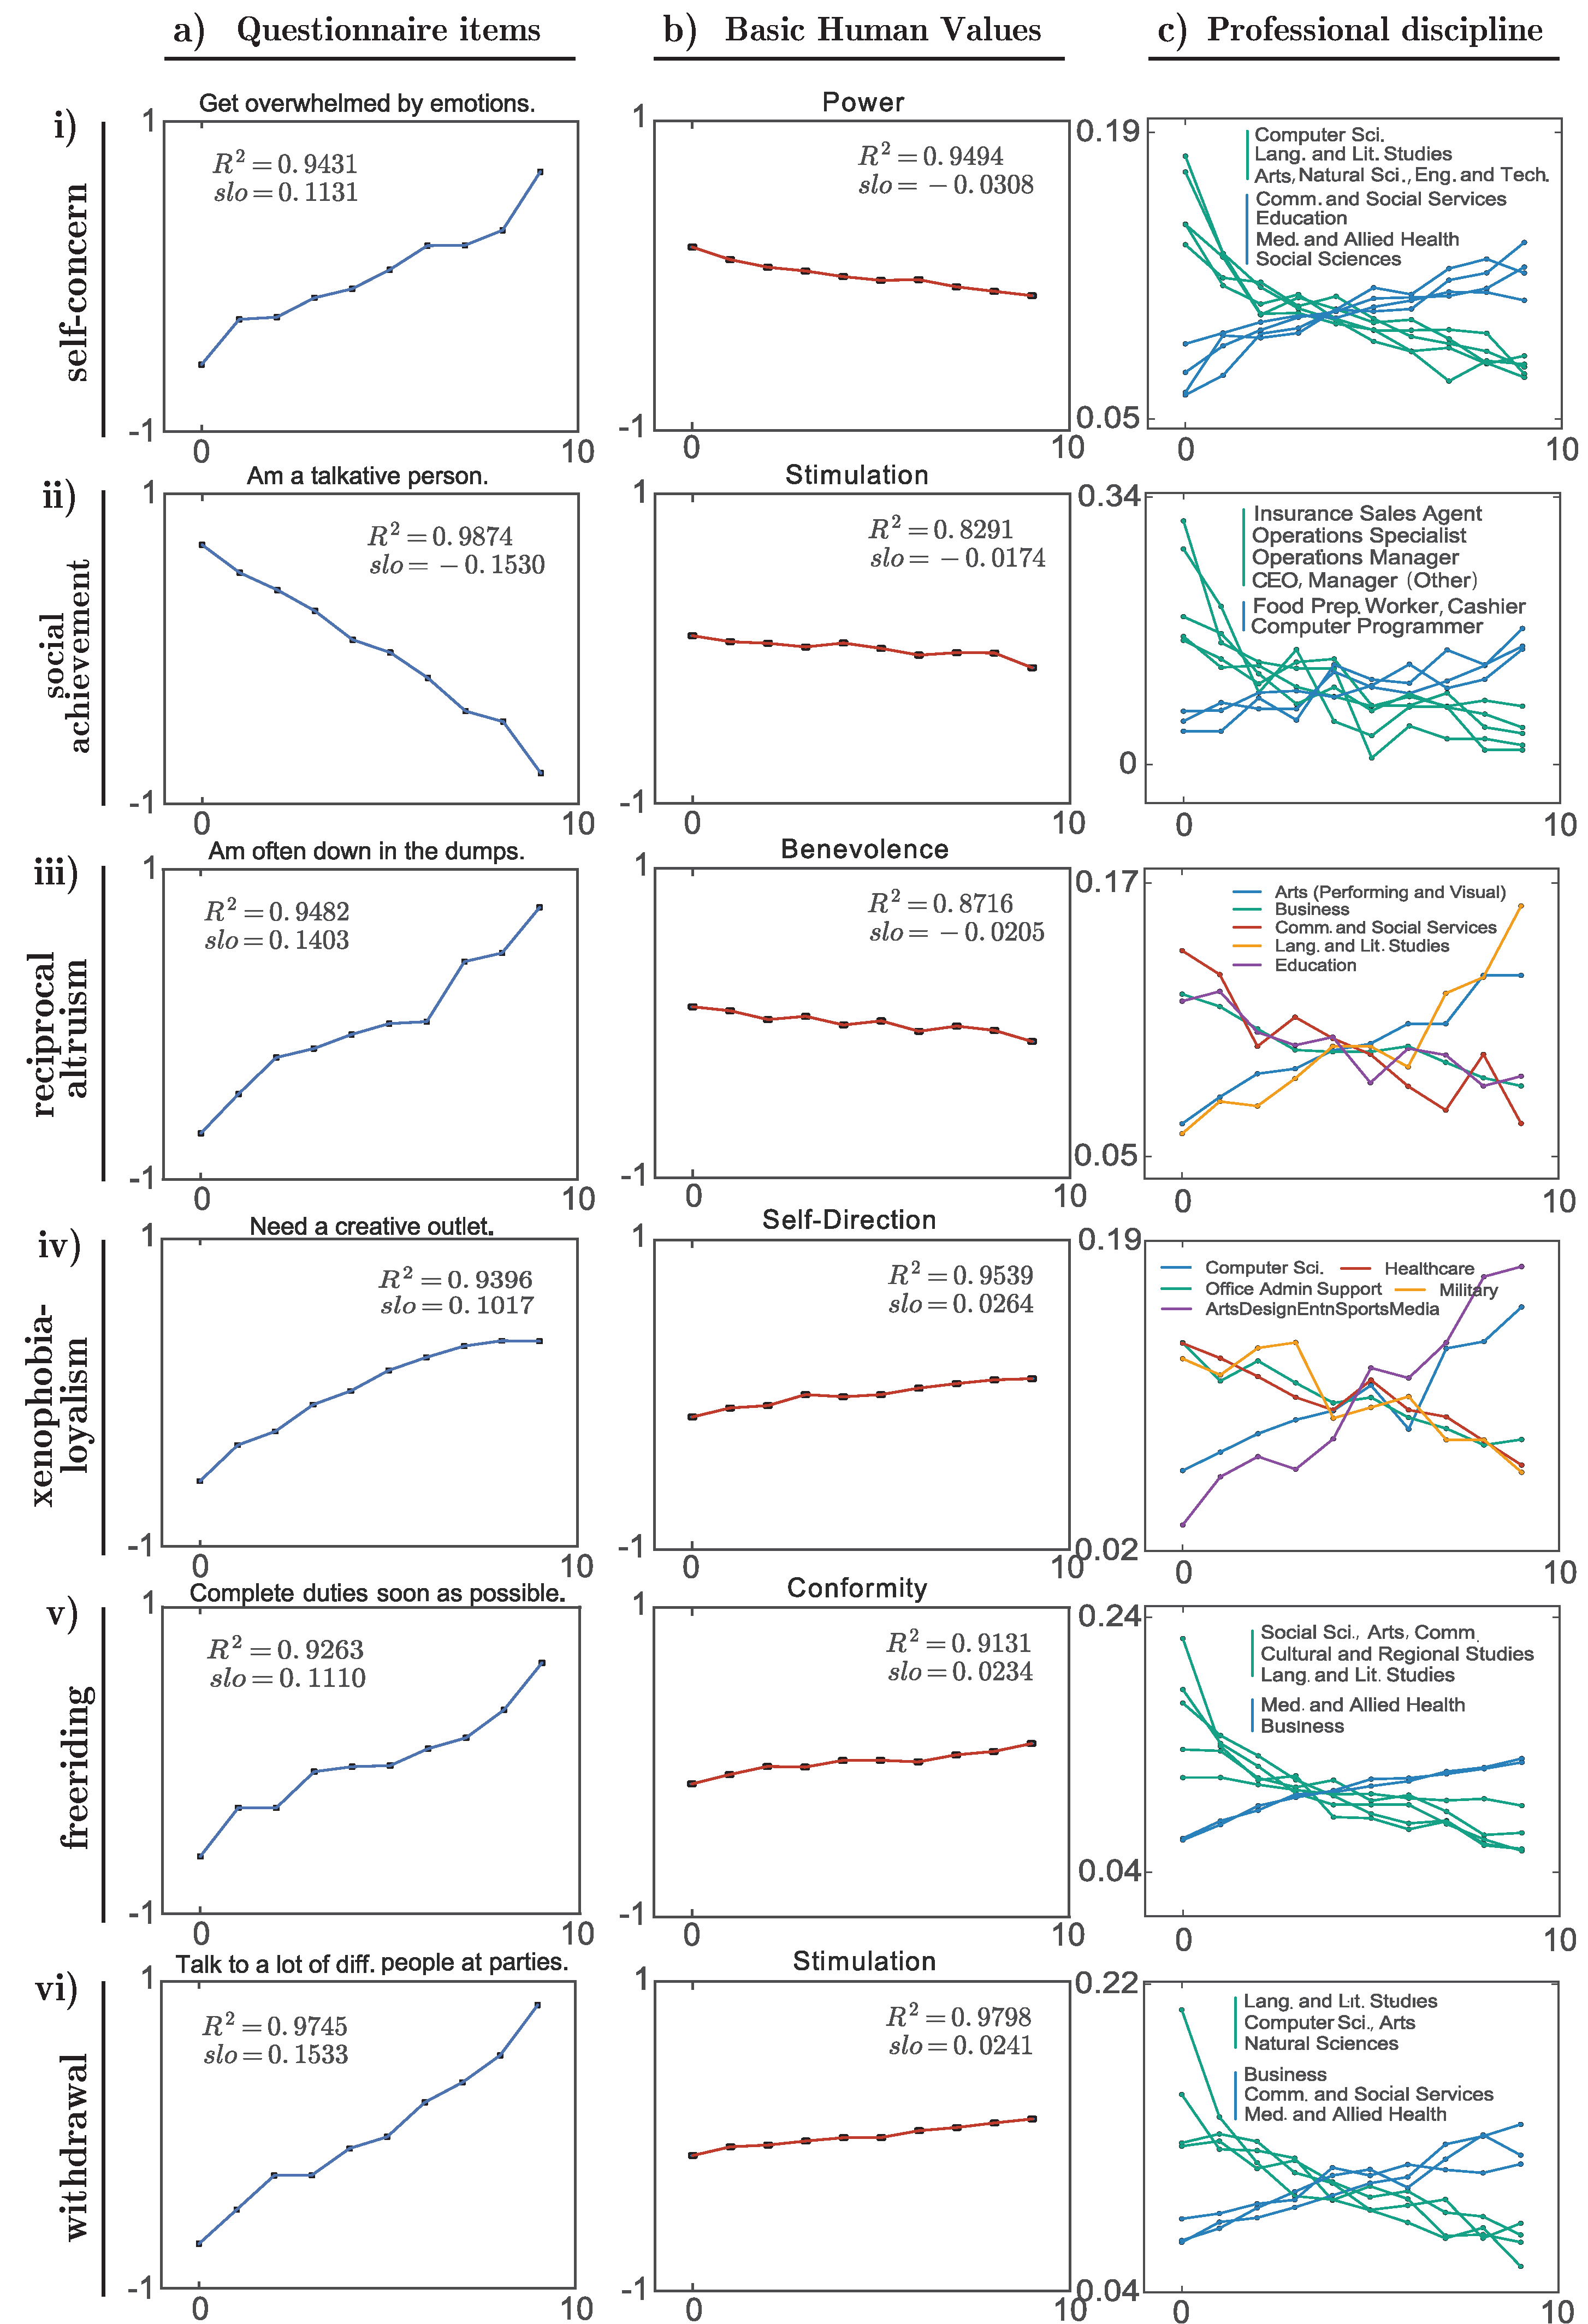
\includegraphics[width=1\textwidth]{figures/firstEnrichmentsQuestionnaireValues}
	\caption{\label{fig:firstEnrichmentsQuestionnaireValues} Enrichments for each archetype. \textbf{a-b)} are single strongest enrichments of questionnaire items ({\color{blue}blue}) and Basic Human Values ({\color{red}red}). \textbf{c)} are enrichments of professional disciplines. First axes are bin-distances from archetype and second axes for a-b) are average item response values rescaled from [1 ; 5] to [-1 ; 1] and normalized frequency for c). 'slo' is the slope of a first order approximation of the curve, so \textbf{negative slope is enrichment and positive slope is depletion}.}
\end{figure}

\begin{sidewaystable}
	% Facets and values
\newcommand{\achFac}{Emotionally stable, unsympathetic, self-concerned, exploitative, arrogant, hard to offend}
\newcommand{\hosFac}{Talkative, social, lively, moody, worrying, emotional, insecure/need reassurance, easily hurt}
\newcommand{\wilFac}{Happy, hard-working, dutiful, well-tempered, trusting, talkative, social, lively, unworried}
\newcommand{\loyFac}{Uncreative, simple-minded, ignorant, unintellectual, slow}
\newcommand{\hipFac}{Undutiful, not hard-working, disorderly, rule-breaker, don't plan ahead, unworried, calm, emotionally stable}
\newcommand{\folFac}{Not talkative, shy, antisocial, reclusive, depressed, worried, moody, irritated, panicking, emotional, lost}

\newcommand{\achVal}{Power, not benevolence, not conformity, not tradition, achievement, stimulation, hedonism}
\newcommand{\hosVal}{Stimulation, hedonism, power, achievement, universalism, security, not conformity}
\newcommand{\wilVal}{Conformity, benevolence, stimulation, achievement, tradition, security, universalism}
\newcommand{\loyVal}{Not self-direction, conformity, not stimulation, tradition, not universalism, security, not hedonism}
\newcommand{\hipVal}{Not security, not achievement, not tradition, not power, not benevolence, stimulation, hedonism}
\newcommand{\folVal}{Not stimulation, not achievement, not conformity, not power, not security, not benevolence, not hedonism, not tradition}

\newcommand{\achBeh}{-}
\newcommand{\hosBeh}{Freq. calls/texts, brief stops, goes new places, long calls, sends more texts than receives, response-rate depends on receiver, socializes at night}
\newcommand{\wilBeh}{Socializes off-campus, freq. calls/texts, goes out at night, unperiodic social pattern, brief stops, gets final word}
\newcommand{\loyBeh}{Periodic social pattern, returns calls/texts, immediate text responses, has long ongoing chats, shows up for class}
\newcommand{\hipBeh}{Short calls, unperiodic social pattern, very nocturnal, interacts with strangers, none/slow text/call responses, doesn't conclude chats}
\newcommand{\folBeh}{Doesn't meet people at campus, not nocturnal, periodic social pattern, rarely calls/texts/looks at phone, few contacts, stays home}

% Attribtues
\newcommand{\achRel}{No}
\newcommand{\achDis}{Computer sci., language and lit., arts, natural sci. eng. and tech. - not communication, edu., med. and health, social services}
\newcommand{\achJob}{Unemployed}
\newcommand{\achExe}{Yes}
\newcommand{\achSmo}{-}
\newcommand{\achAge}{Younger (0.5 years/bin), not retired}

\newcommand{\hosRel}{Yes}
\newcommand{\hosDis}{Insurance sales, operations manager/specialist, CEO - not food preparation worker, cashier, computer programmer}
\newcommand{\hosJob}{Employed}
\newcommand{\hosExe}{Yes}
\newcommand{\hosSmo}{Yes}
\newcommand{\hosAge}{Not retired}

\newcommand{\wilRel}{Yes}
\newcommand{\wilDis}{Business, education, community and social services - not arts, lang. and lit.}
\newcommand{\wilJob}{Employed, not student}
\newcommand{\wilExe}{Yes}
\newcommand{\wilSmo}{No}
\newcommand{\wilAge}{Older (-1.01 years/bin)}

\newcommand{\loyRel}{Yes}
\newcommand{\loyDis}{Healthcare, office support, military - not computer sci. and arts}
\newcommand{\loyJob}{Student, unemployed}
\newcommand{\loyExe}{-}
\newcommand{\loySmo}{No}
\newcommand{\loyAge}{Younger (0.3 years/bin)}

\newcommand{\hipRel}{No}
\newcommand{\hipDis}{Arts, cultural and regional studies, lang. and lit. studies, communication, social sci. - not business and med./health}
\newcommand{\hipJob}{Student, unemployed}
\newcommand{\hipExe}{No}
\newcommand{\hipSmo}{Yes}
\newcommand{\hipAge}{Younger (0.6 years/bin), not retired}

\newcommand{\folRel}{No}
\newcommand{\folDis}{Arts, lang. and lit., computer sci., natural sci. - not business, health-care and communication}
\newcommand{\folJob}{Unemployed}
\newcommand{\folExe}{No}
\newcommand{\folSmo}{No}
\newcommand{\folAge}{Retired}

% Row-titles
\newcommand{\achtit}{\textbf{\achiever}}
\newcommand{\hostit}{\textbf{\host}}
\newcommand{\wiltit}{\textbf{\wildcard}}
\newcommand{\loytit}{\textbf{\loyalist}}
\newcommand{\hiptit}{\textbf{\hippie}}
\newcommand{\foltit}{\textbf{\follower}}

\newcolumntype{?}{!{\vrule width 1.5pt}}
\newcommand{\mcc}[1]{\multicolumn{1}{c}{\textbf{#1}}}
\newcommand{\mccrl}[1]{\multicolumn{1}{c?}{\textbf{#1}}}

% Table
{
\footnotesize
\hspace*{-1.8cm}
\begin{tabular}{C{1.7cm}|C{2.6cm}?C{3.0cm}?C{2.7cm}|c|C{1.5cm}|c|c|C{1.5cm}?C{2.7cm}|}
\mcc{}		& \mcc{\normalsize Facets}	& \mcc{\normalsize Values}	& \multicolumn{6}{c}{ \textbf{\normalsize Demographic attributes}}												& \mcc{\normalsize Mobile behavior}	\\ \cmidrule[1pt]{2-10}
\mcc{}		& \mccrl{Highlights}		& \mccrl{Highlights}		& \mcc{Discipline}	& \mcc{Rel.ship} 	& \mcc{Job status} 	& \mcc{Exerc.} 	& \mcc{Smok.}		& \mccrl{Age} 	& \mcc{Highlights}		\\ \cline{2-10}
\achtit		& \achFac 					& \achVal 					& \achDis 			& \achRel 			& \achJob		 	& \achExe 		& \achSmo 			& \achAge 		& \achBeh				\\ \hline
\hostit 	& \hosFac 					& \hosVal 					& \hosDis 			& \hosRel 			& \hosJob		 	& \hosExe 		& \hosSmo 			& \hosAge 		& \hosBeh				\\ \hline
\wiltit 	& \wilFac 					& \wilVal 					& \wilDis 			& \wilRel 			& \wilJob		 	& \wilExe 		& \wilSmo 			& \wilAge 		& \wilBeh				\\ \hline
\loytit	 	& \loyFac 					& \loyVal 					& \loyDis 			& \loyRel 			& \loyJob		 	& \loyExe 		& \loySmo 			& \loyAge 		& \loyBeh				\\ \hline
\hiptit		& \hipFac 					& \hipVal 					& \hipDis 			& \hipRel 			& \hipJob		 	& \hipExe 		& \hipSmo 			& \hipAge 		& \hipBeh				\\ \hline
\foltit	 	& \folFac 					& \folVal 					& \folDis 			& \folRel 			& \folJob		 	& \folExe 		& \folSmo 			& \folAge 		& \folBeh				\\
\cmidrule[1pt]{2-10}
\end{tabular}
}
	\caption{\label{tab:facetsValuesAttributesTable}Summary table of the strongest significant enrichments for facets, Basic Human Values, demographic attributes and mobile behaviors for each archetype. Considering the rows one by one there are clear differences between the archetypes. Facets, values and behaviors are sorted by descending enrichment/correlation strength. The following words are shortened: sci[ence], tech[nology], eng[ineering], lit[erature], lang[uage], edu[cation] and med[icine]. '-' symbolizes no significant enrichments. Facets are single-word descriptions of longer questionnaire items (see Appendix \ref{app:questionnaireEnrichmentTable}). Demographic attributes strongly influenced by age, such as education level and marital status, are omitted due to the strong age differences between archetypes.}
\end{sidewaystable}

Two datasets provide facets, values and attributes and one provides behavior.
The SAPA-project dataset is analyzed for facets and demographic attributes.
It comprises personality test responses from a large number of Internet users, as well as demographic information such as age, gender, country, education and marital status.
This provides a unique opportunity to study how personality - or in this paradigm, distance to an archetype - links to demographic attributes.
Furthermore the property that the SAPA collection method asks respondents questions from multiple inventories is taken advantage of.
When analyzing enrichment of QIs care has been taken to avoid "circular enrichment" since distance is measured in units of BFTs and BFTs are composed of QIs.
By analyzing enrichment of QIs from the SPI inventory for individuals close to each archetype, where distance is measured using BFT values computed from the IPIP100 inventory, circularity is mitigated. 

The \textit{myPersonality} Facebook dataset is analyzed for values.
The SensibleDTU dataset is analyzed for behaviors.
Raw data is recombined into 38 behavioral indicators for 412 study participants, using an - for the purpose of this study - extended version of the behavioral feature extraction Python software \textit{bandicoot}. The indicators can be viewed in Appendix \ref{app:fullListOfExtractedFeatures}, and the implementation pipeline is presented in Section \ref{subsubsec:featureEngineering}.

		\subsubsection{Summary and strategy suggestions \label{subsubsec:summary}}
		The analysis yields a large number of enrichments and correlations for each archetype, of which an excerpt is visualized in Figure \ref{fig:firstEnrichmentsQuestionnaireValues}, a shortened overview is shown in Table \ref{tab:facetsValuesAttributesTable}, and elaborate presentation is given in Appendices \ref{app:questionnaireEnrichmentTable}-\ref{app:behaviorCorrelationTable}. 
Here, each archetype is presented in prose highlighting their individual characteristics.
Each is examined and proposed a behavioral strategy with reference to existing literature when possible (primarily \textit{Evolutionary Psychology} (2014) by Workman et. al.\mcite{workman2014evolutionary}).


\subparagraph*{Self-concern}
The \achiever archetype is unemotional and mostly interested in power and achievement.
Occupied in fields which commonly don't involve working directly with people, whereas the depleted professional disciplines are the reverse.
Lacks sympathy, tends to exploit others for own ends and looks down on others.
Has a high degree of control through emotional stability and is hard to offend.
Highest valued BHVs other than power and achievement are stimulation and hedonism and least valued BHVs are benevolence, conformity and tradition.
Tends to be slightly younger (\textasciitilde5 years younger than furthest bin), particularly not retired individuals, not committed in relationships and has a tendency to exercise often.
Comprises many unemployed individuals.
There were found no significant correlations between distance from this archetype and behaviors measured through smartphones.

	\subparagraph{\textnormal{\textit{Discussion}}} 
	These are traits that are often prevalent in individuals with antisocial personality disorders (APD) and are typically lumped together using the term \textit{psychopathy} by evolutionary psychologists\mcite{workman2014evolutionary}.
	People suffering from psychopathy, i.e. \textit{psychopaths}, can use their manipulative tendencies to exploit others, gaining resources including sex, which is supported by studies that show ADP traits to correlate positively with an accelerated mating strategy\mcite{jonason2009dark, jonason2011mate}.
	Psychopathic traits are furthermore shown to lead to success in high-level business positions\mcite{hare2006psychopathy}, which the current results, however, don't support.
	Enriched disciplines are rather those of solitary nature, and as such it is just as reasonable to speculate this archetype to have a form of passive aggressive withdrawal strategy, that don't necessarily attract only attract psychopaths and individuals with other personality disorders.
	Furthermore, considering Figure \ref{fig:consensusArchetypes}.b distances to this archetype are typically small, which in other words mean that many people somewhat resemble this archetype, which is inconsistent with the converging agreement between psychologists that only up to 3\% of any larger population should suffer from sub-clinical psychopathy\mcite{kring2005abnormal}.
	As such it might be an artifact of a possible tendency in many humans to be competitive and, depending on context, feel emotions of contempt and superiority towards others, all of which may only surface when filling out a survey.
	The safest label for this strategy is therefore \achiever.

\subparagraph*{Social-achievement}
The \host archetype is highly social, talkative and lively, yet suffers from mood swings, insecurity and gets hurt easily.
Values are mostly stimulation, hedonism, power and achievement.
Has high level of employment and works high-pace jobs that directly involve people, such as sales, management and CEO positions.
Does not hold unskilled positions (food prep. worker, cashier) which resonates with the valuing of achievement and power.
Curiously both smokes and exercises, which is somewhat contradictory but can be explained by the high held value of stimulation and hedonism.
It may also indicate an ability to hold contradictory beliefs simultaneously, which is undoubtedly a useful feature for individuals whose behavioral strategy is to use social engagement to advance in hierarchies.
Maintains social relations through mobile phone by calling and texting a lot, socializes and moves around frequently both day and night and explores new places (visits places only once).
Typically makes long calls, sends more texts than receives and response-rate to texts or missed calls tends to depend on who the receiver is.

	\subparagraph{\textnormal{\textit{Discussion}}}
	The BFTs and enrichments for this archetype resonate with with known literature.
	Recall that this archetype is characterized by high levels of \OPE, \EXT and \NEU.
	\NEU is found to correlate positively with competitiveness and academic success for those who are resilient enough to cope with it\mcite{ross2001imposter, mckenzie2000neuroticism}, which agrees with the finding that this archetype works in fast-pace/high-status jobs such as CEO and operations manager.
	Provided that the goals of this archetype are mainly achievement and power (curiously similar to the \achiever archetype), is seems clear that this strategy focuses on using social interaction as a tool for acquiring resources and power.
	To the knowledge of this author there is no strategy treated in EP literature which strongly resembles this one.
	It can be argued that this strategy may attract individuals with multiple complex profiles, since it is a fairly universal drive to be highly social - and if one is also sensitive interacting with people may be a matter of earning popularity and using vulnerability to get ahead. This is discussed by Nettle\mcite{nettle2006evolution}.
	On a highly speculative note, given the occupation profiles, it might even attract psychopaths.
	However, for now it is simply named after its main facet \textit{social} and value \textit{achievement}.


\subparagraph*{Reciprocal altruism}
Happy, lively and social, well-tempered, not worried, trusting, hard-working and dutiful describe the most diverse set of enriched facets for the \wildcard archetype.
It highly values conformity, benevolence, stimulation and achievement, and is strongly enriched for relationship commitment and employment.
This archetype is more mature in age (closest bin is \textasciitilde10 years older than furthest bin), and tends to work in disciplines that have direct interaction with people.
Smoking is depleted and exercise is enriched, indicating self-discipline.
Has many friends outside of the university, frequently uses phone for communication, goes out at night, doesn't meet people in predictable weekly pattern, goes to many different places and tends to send the last text in chat conversations.

	\subparagraph{\textnormal{\textit{Discussion}}}
	EP build on the notion reciprocal altruism first introduced by Trivers\mcite{trivers1971evolution}. The idea, which is also mentioned briefly in Section \ref{subsubsec:individualDifferencesAndPersonality}, is that altruism may have developed as a mechanism for optimizing group fitness, or simply as a personal strategy for storing value by giving it away and expecting a return of similar value at a later time of greater need. Much about this archetype resemble this, and as such it is deemed to represent \textit{reciprocal altruism}.

\subparagraph*{Xenophobia-loyalism}
The \loyalist archetype is uncreative, simple-minded and slow, values conformity, tradition and security and neither self-direction, stimulation nor hedonism.
Works in health-care, office administration support and military, and particularly not computer science and arts.
Slight tendency to be younger (\textasciitilde3 years younger than furthest bin), non-smoker, committed in relationship and also often students.
Meets people in predictable weekly pattern, immediately responds to missed calls/texts, has long ongoing chats and shows up for class.

	\subparagraph{\textnormal{\textit{Discussion}}}
	Workman makes the remark that \textit{"Social psychologists have long known that the roots of xenophobia, or hatred of strangers, may be traced back to identifying strongly with one's own group and negatively stereotyping those of other groups."}. Going further back Darwin once noted: \textit{"The tribes inhabiting adjacent districts are almost always at war with each other [and yet] a savage will risk his own life to save that of a member of the same community."}\mcite{darwin1888descent}.
	Several enriched features of this archetypes resonate with characteristics commonly associated with xenophobia and loyalism. So the question of why this seemingly negative-sounding characterization should be an ESS for performing life's many tasks in such a way to increase fitness is fairly difficult to answer. Possibly this is remanence of a time where we lived in small tribes and had to react strongly to outsiders to survive, as noted by Darwin.
	However, others suggest that the ability to perceive sharp distinctions between "us and them" group members is crucial to the formation of lasting coalitions and is therefore an adaptive strategy\mcite{krebs1997social}.

\subparagraph*{Freeriding}
The \hippie archetype is undutiful, disorderly, not hard-working, breaks rules, unworried, emotionally stable and does not plan ahead.
Only values stimulation and hedonism, and particularly doesn't value security, achievement, tradition, power nor benevolence.
Professional disciplines that are enriched near the archetype include performance and visual arts, cultural studies, language and literature studies as well as communications and social science, while there is depletion for business and medicine/health related disciplines.
This archetype is younger (\textasciitilde6 years younger than furthest bin and not retired), not committed in relationship, tends to smoke and not exercise, and is enriched for student and unemployed.
Makes short calls, doesn't meet people in predictable weekly pattern, is very nocturnal, interacts with strangers and bad at responding to missed calls/texts.

	\subparagraph{\textnormal{\textit{Discussion}}}
	Workman remarks:
	\textit{"The evolution of cooperation among non-kin is greatly compromised by the existence of freeriders. Freeriders reap the benefits of cooperation without paying the costs and thus place themselves at a competitive advantage by exploiting cooperators. Many (e.g. Tooby et al., 2006)\mcite{tooby2006cognitive} have argued that, given the inherent disadvantages of cooperating with freeriders, cooperation could not have evolved unless mechanisms for detecting and dealing with freeriders also evolved."}
	While the behavior of the freerider - other than its immediate strategy - are not examined in literature, this archetype could be a candidate, to help probe further into the understanding of this strategy which relies on others to do the heavy lifting.

\subparagraph*{Withdrawal}
The \follower archetype is antisocial and reclusive, worried, depressed, suffers from mood swings and gets very emotional.
Values none of the BHVs, and particularly not stimulation, achievement, conformity and power.
Disciplines include arts, language and literature, computer science and natural sciences, and particularly not human interaction dependent disciplines in business, health-care and communication.
No significant enrichment of age, but enriched for unemployment and retirement which indicates that this strategy might attract older people.
Neither smokes nor exercises, which resonates with the low valuing of stimulation and hedonism, and is not committed in relationship.
Doesn't meet people at campus, not nocturnal, meets people in predictable weekly pattern, rarely calls/texts/looks at phone, has few contacts, stays at home.

	\subparagraph{\textnormal{\textit{Discussion}}}
	This archetype may also simply be called \textit{depression}. Models in literature view depression as adapted response to adverse conditions, which may help the individual accept defeat\mcite{wolpert2008depression}.
	Others attribute it more complexity, arguing that it is an involuntary strategy to signal yielding towards the surroundings such as to terminate unnecessary conflict (which would otherwise likely have been lost by the depressed)\mcite{price1994social}. If the latter is true, the label \textit{withdrawal} is appropriate.


	% Supervised Learning
	\newpage
	\subsection{Archetypes separate data better than traits \label{subsec:classification}}
	To investigate how well the the archetypes, which perform the suggested strategies, seperate data, the predictive power of archetypes as a target variable in a supervised learning paradigm is investigated. The prediction accuracy is compared to that of plain BFTs as well as PCs of QIs, of which there are also six. Data from the SensibleDTU experiment is used. As is shown in Section \ref{subsubsec:analysisAndData}, different strategies tended to be adopted by people in different age groups, and since the population in the SensibleDTU dataset is strictly composed of students, conclusions must be drawn with a degree of respect for this bias. Details of the analysis are are discussed in Section \ref{subsec:classification}.

Optimized prediction models are trained on 38 indicators to predict low, medium or high distance to each of the archetypes. Figure \ref{fig:classification_results_CA} visualizes the accuracies, and explains high-level aspect of the applied procedure. It is compared to prediction accuracies for Big Five traits (Figure \ref{fig:classification_results_BFT}) and PCs of Big Five Inventory QIs (Figure \ref{fig:classification_results_PCA}) using the same approach. There are discovered to be six PCs in QI-space as shown in Figure \ref{fig:significantPCs}. The remainder of this section presents the results.

\textbf{Distances to archetypes are predicted with highest accuracies}.
Average prediction accuracies above baseline (AB) reported in Figure \ref{fig:classification_results_CA}, \ref{fig:classification_results_BFT} and \ref{fig:classification_results_PCA} are 5.8\%, 2.4\ and 4.1\%, respectively. As such PCs can be predicted better than BFTs and distance from archetypes can be predicted better than PCs. Prediction accuracy compares to, but is not better than what has already been reported for prediction of BFTs in previous studies\mcite{monsted2016phone, de2013predicting}. This may be upsetting in terms of the predictive promise of the behavioral indicators computed using the extended version of the bandicoot software (see Section \ref{subsubsec:featureEngineering}), but on the other hand it also shows that archetypes do split the data better.

\begin{figure}[b]
	\centering
	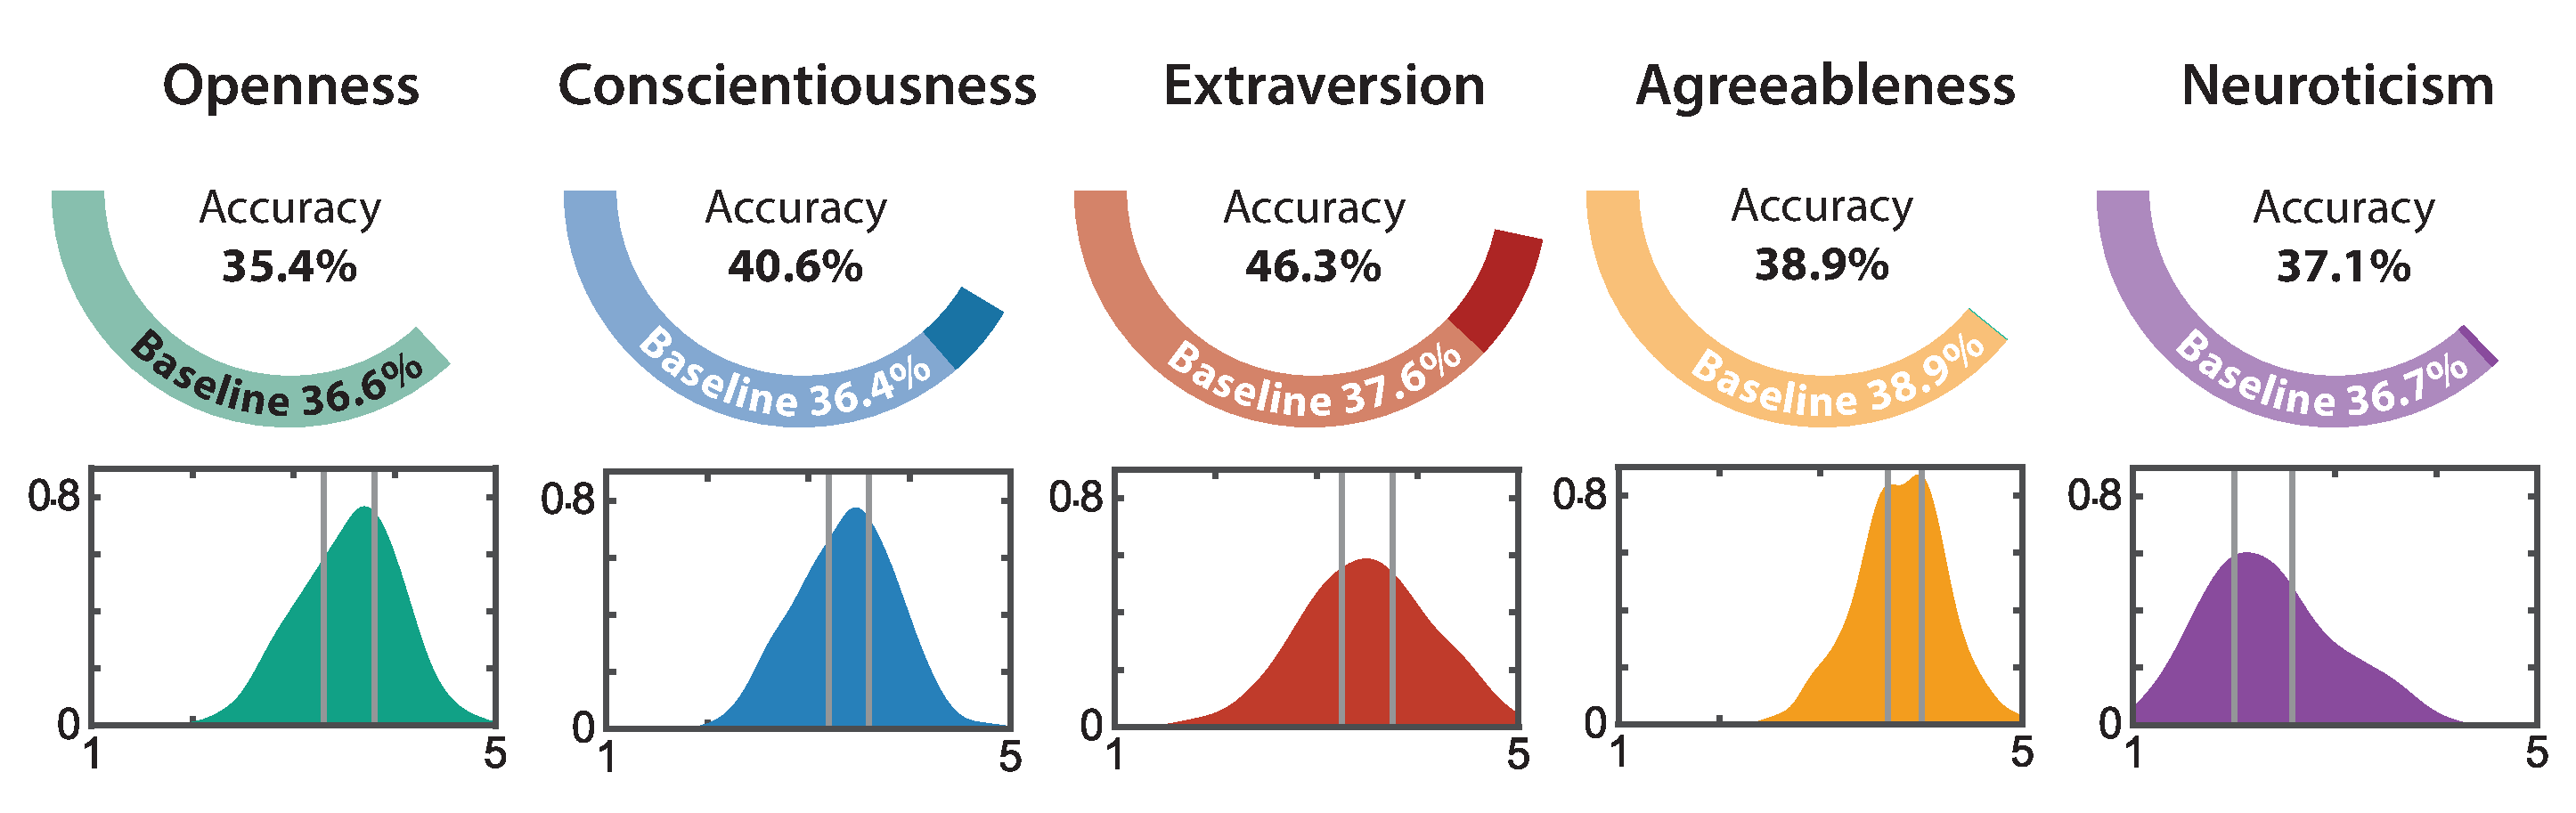
\includegraphics[width=\textwidth]{figures/classification_results}
	\caption{\label{fig:classification_results_BFT} Three-class classification accuracy of BFTs predicted from behavioral indicators. Only C and E can be predicted Same procedure as described in Figure \ref{fig:classification_results_CA}.}
\end{figure}

\textbf{Archetypes are predicted better than their parts}.
In the current approach only \CON and \EXT can be predicted well. Considering the \achiever archetype, prediction accuracy is 6.8\% AB, yet out of these two BTFs this archetype only varies on \CON which has prediction accuracy 4.2\% AB. It is unclear what accounts for this difference, and further analysis is requires to understand it. 

\begin{figure}[h!]
	\centering
	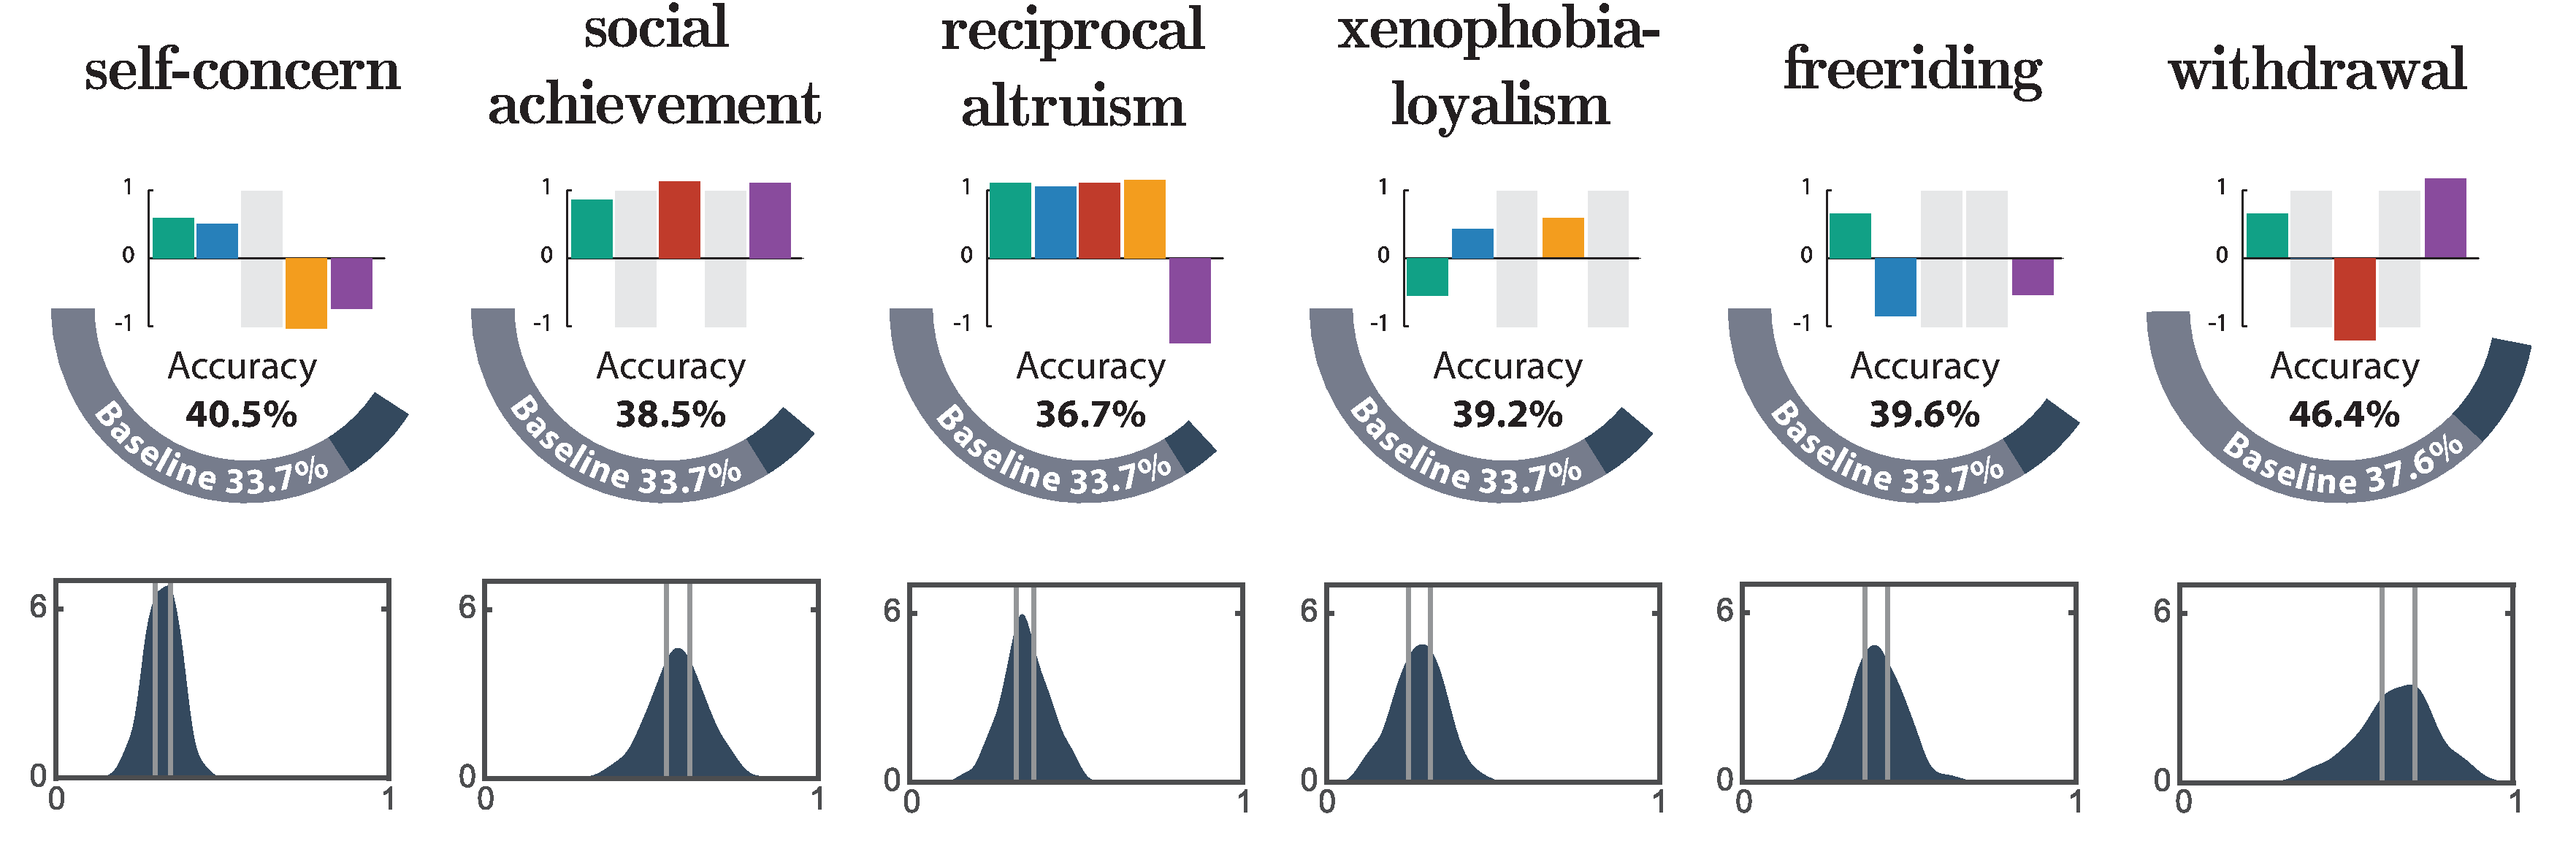
\includegraphics[width=\textwidth]{figures/classification_results_CA}
	\caption{\label{fig:classification_results_CA} Three-class classification accuracy of archetypes predicted from behavioral indicators. Samples are split into three semi-balanced classes based on their target values (low, medium, high). Sample distributions are shown as KDE plots below each score diagram, and vertical lines show decision boundaries. Reported accuracies are averages over 100 shuffled stratified cross validation folds of parameter optimized random forest models (random search and grid search), with standard errors in the range of .2 to .5 percent. Baselines are calculated as the of size of the largest class divided by number of samples. The bar diagrams show how each component/archetype is interpreted in terms of BFTs, where height is the normalized archetype position in BF space and non-consensus dimensions are shown in grey.}
\end{figure}

\begin{figure}[h!]
	\centering
	\begin{minipage}[l]{0.5\textwidth}
		\flushleft
		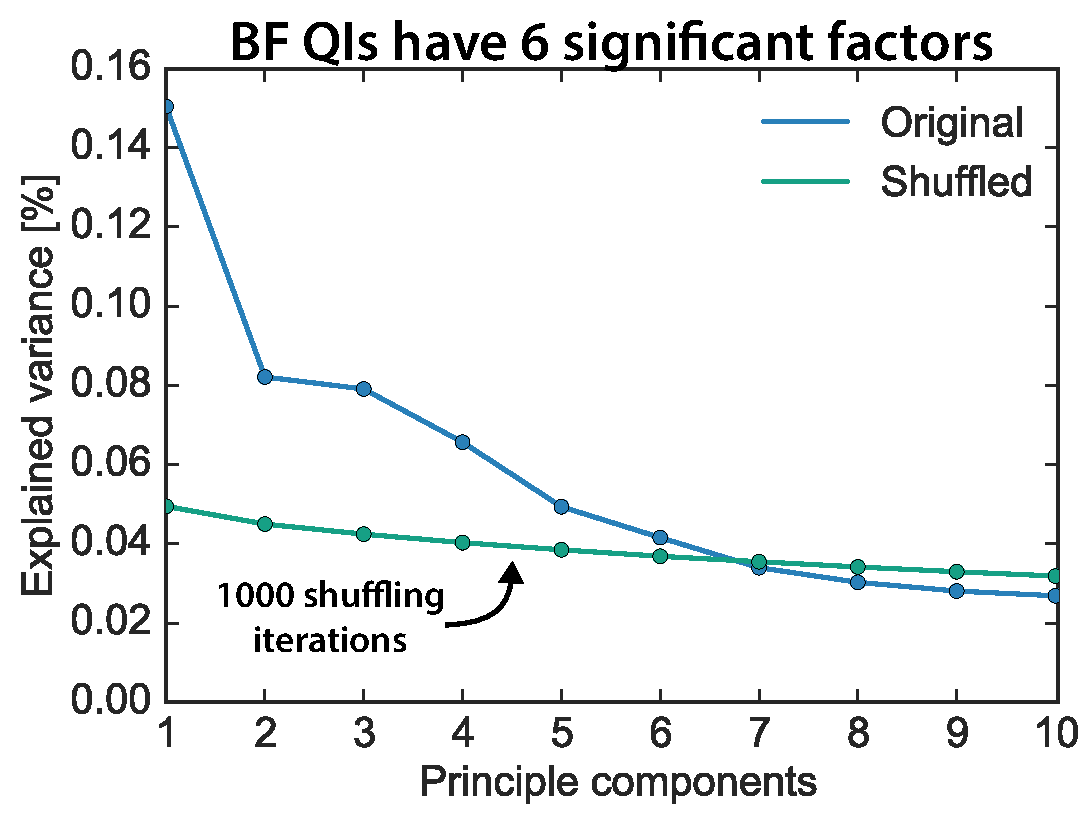
\includegraphics[width=0.95\textwidth]{figures/significantPCs}
	\end{minipage}
	\begin{minipage}[r]{0.49\textwidth}
		\flushright
		\caption{\label{fig:significantPCs}Percentage variance explained of PCs for original and domain shuffled Big Five questionnaire items. The green curve results from 1000 shuffling iterations which are plotted with high transparency. It shows that the six first principle components in Big Five questionnaire item space are significant, because none of the shuffling iteration can produce components of higher explained variance than the first six.}
	\end{minipage}
\end{figure}

\begin{figure}[h!]
	\centering
	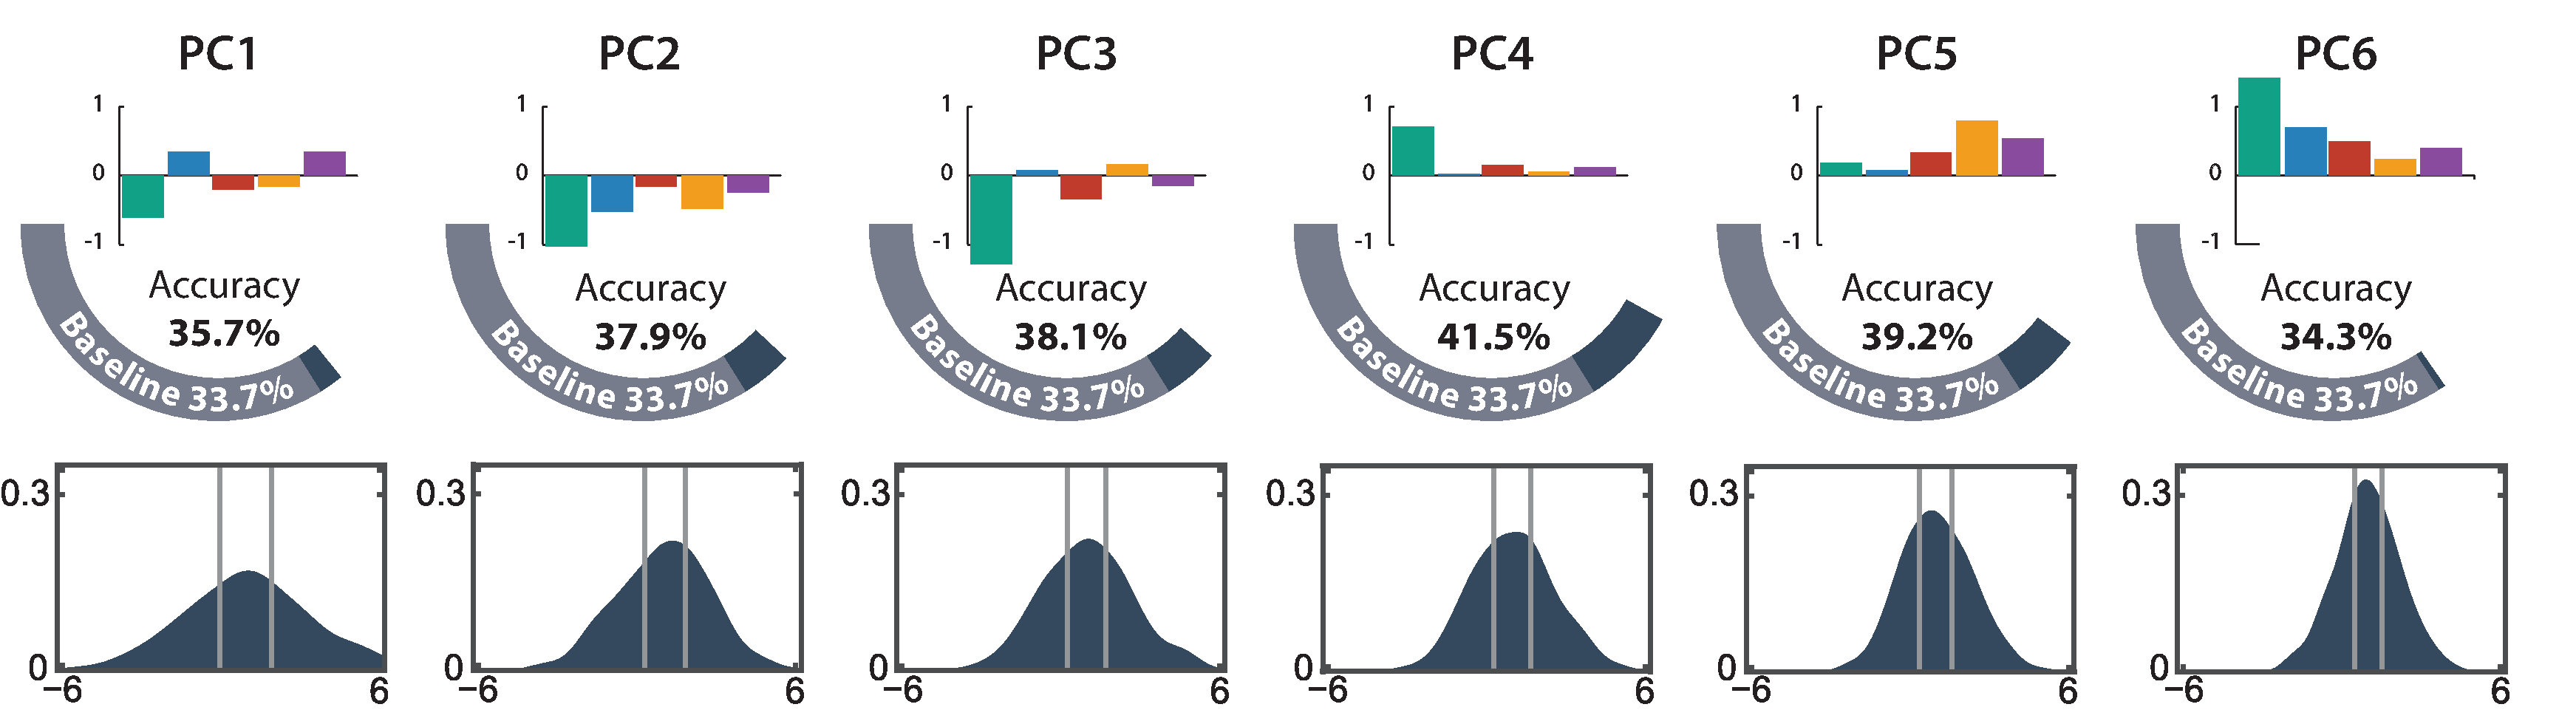
\includegraphics[width=\textwidth]{figures/classification_results_PCA}
	\caption{\label{fig:classification_results_PCA} Three-class classification accuracy of PC components of Big Five Inventory QIs\cite{facet54big}. Same procedure as described in Figure \ref{fig:classification_results_BFT}. The bar diagrams show how each component/archetype is interpreted in terms of BFTs. Bar length correspond to inner products between PC and BF trait.}
\end{figure}


\newpage
\setcounter{figure}{0}
\thispagestyle{plain}


% Discussion
% ----------
\newpage
\section{Discussion \label{sec:discussion}}
Out of the six archetypes which have been suggested based on the conducted analysis, all except the \host archetype appears to fit a strategy known from the literature. There are, however, a number of aspects which are important to the validity of the results which needs to be discussed. Some are scientific in nature and some regard the ethical implications.

\textbf{The Big Five model is "too crude" to capture fine-grained strategies}.
The Big Five factors result from factor analysis based in as many as 17.000 personality descriptive adjectives (English language), each of which was encoded into language arguably to fill some hole in comprehension. The model then lumps together all these words, into five factors that admittedly comprise a whole range of facets, but at the same time disregards much of the variance inherent to the language. For this reason, very fine-grained personality differences cannot be explained. For example, there is no trait in the Big Five model that successfully captures a persons psychopathic tendencies to form close relationships with people for the sake of personal gain. Trying to describe this behavior using the Big Five model is like trying to grab a coin with a boxing glove. As such, the strategies which are suggested in this work, are never less crude than the model they were inferred from.

% \textbf{The strategies are broad}.
% This relates to the above statement.
% Comparing to strategies treated in e.g. game theory, the ones suggested in this study are fairly broad spectered. This is to say, a strategy such as the \host could comprise any number of otherwise vastly different individuals. There might even me a few psychopaths in there. As such it shows personality strategies to be very unspecific constructs. Just because one knows the personality of another person their behavior might still be a mystery.

\textbf{Archetypes are not real people}.
There is an important notion to be made about the nature of these archetypal personalities. When presenting this work to people who are not familiar with it, and in particular when showing people the archetypes they have a strong tendency to quickly identify with one. Why people do this remains an open question but a speculation is that people may find it easier to understand things such as this by projecting their own self-image and feelings onto it. However, while people tend to do this, no one can really be described by just one archetype. In fact, by a geometrical argument (and as can be seen from Figure \ref{fig:consensusArchetypes}.b), no one is very close to an archetype - we are all described by \textit{all} archetypes at the same time. That is to say, since the archetypes were derived from the point distribution of personalities in Big Five space using the PCHA algorithm run with some allowed slack, points are generally closer to the middle of the simplex than they are to the archetypes.

\textbf{People are not necessarily stuck with a strategy}.
This study makes no claims about human nature beyond the strategies which can be inferred from the data. That is to say, whether a person can change strategy over a short period of time, or instantly depending on context, this study does not know. However, it does say that no person can fully assume more than one strategy \textit{at a time}. Picturing the Pareto front in 3D trait-space, this makes sense - a point can only be in one location at a time. Yet, the result that the \wildcard archetype tends to be far older than e.g. the \hippie suggests that people do change strategies over a lifetime.

% \textbf{Strategy fits niche and niche fits strategy}.
% The question of causality in terms of how strategy finds a niche is important.
% One may ask whether people with a certain strategy is drawn towads a particular niche or whether the niche people find themselves in shapes their strategy.
% The answer should be that it goes both ways.
% Personality psychology teaches that personality traits are 30-50\% inheritable which means that up to 70\% of a persons personality is adapted.
% As such there is a component of ones personality that draws one towards the most appropriate niche, 
% One may ask whether the \achiever archetype tends to be unemployed because it dislikes other people, or dislikes others because it tends to be unemployed.
% People are therefore both in control and not in control over their personalities, and this gives rise to the important notion that a persons niche 

\textbf{The type of people who take surveys on the Internet may not represent a general population}.
This very artifact may be what causes the distribution of traits to be so different between datasets that were collected online and per phone, as shown in Appendix \ref{app:BFdist}. However, it is unknown exactly how severe this biases the data, or if it biases it at all.

\textbf{Archetypes separate data better than traits do, but is this really so surprising?}
This short discussion would have been replaced by a simulation if time had permitted it. However, since that is not the case a few remarks on the result that archetypes are better prediction targets than BFTs and QI-PCs are due. First: Maybe it's not so strange? Archetypes are geometrical extremes and the data is not well-seperated so possible the best way to distinguish points is my learning which their nearest archetype is.

\textbf{Confirmation bias may have influenced the analysis}.
We are all humans. And as humans analyzing humans we are constantly at risk of making analysis choices that are under bias of this fact. So while care has been taken to withdraw excitement over preliminary results and "read too much into things", it cannot be rejected that some scientifically unhealthy humanity has seeped into the interpretations of the results.

% Conclusions
\newpage
\section{Conclusions \label{sec:conclusions}}
Rooted in the notion from evolutionary psychology that personality is an adapted behavioral strategy, the goal of thesis was to discover these strategies using the Pareto Task Inference paradigm. In the process of conducting this project a number of conclusions were drawn. Each is presented below.

\begin{itemize}
	\item Simulation examples revealed the search for more than six archetypes computationally unfeasible unless a very large number of datapoints is available. This was further exemplified by illustrating that points on the convex hull of a data cluster are not contained within the Pareto front. While this constitutes an upper limit to the number of archetypes, it was argued that for Big Five personality data in five dimensions, the lower bound on number of archetypes should also be six.
	\item Using the same approach for computing archetypes in seven different datasets, six very similar personality archetypes emerged. The most deviating traits were taken to be "not in consensus" meaning they were left variable such that computing distance to the archetypes would disregard non-consensus trait.
	\item Archetypes were found to influence different variables to become enriched or depleted near them. Similarly many behavioral indicators measured through personal smartphones and computed using an extended version of the \textit{bandicoot} software were found to correlate both positively and negatively with distance from archetypes.
	\item Six evolutionary behavioral strategies were suggested for the archetypes based on enrichments correlations. By reviewing the literature, four were to correspond to speculated strategies known to evolutionary psychologists already. This implies that: (1) the Big Five model is in fact an evolutionarily plausible way of carving up personality as argued by Buss\mcite{buss1991evolutionary, larsen2008personality}, and (2) two strategies \achiever and \host which are not accounted for in the literature may be a discovery that can lead to a better understanding of personality as behavioral strategy.
	\item There are significant age differences between behavioral strategies, indicating that humans adopt different strategies over the course of a lifetime.
	\item An individuals' distance to the inferred archetypes can be predicted with greater accuracy than its BF trait values and questionnaire item principal component values. Whether this points to something "special" is discussed, yet remained unanswered and requires more analysis.
	\item Principle components of personality questionnaire items provide a better prediction target indicating that strategies may belong in a PC-basis space rather than a BF-basis space.
\end{itemize}

Furthermore, the project yielded the following general value propositions.

\begin{itemize}
	\item An extended version of the \textit{bandicoot} behavioral indicator software for Python which can readily be applied by other researchers with access to the SensibleDTU dataset, to compute out-of-the-box measures of behavior.
	\item A fast Python implementation of the AA algorithm developed by M\o rup et. al.\mcite{morup2012archetypal}, which is made available on PyPi\mcite{pypcha} and can be installed in any Python environment using the \textit{pip} package manager with the following command: \texttt{pip install py\_pcha}.
\end{itemize}

	% Future Research
	\subsection{Future Research \label{subsec:futureResearch}}
	Since this is an ongoing research project, there is a long list of problems to address which were not investigated or reported in this thesis. The list below presents the most important of those.

\begin{itemize}
	\item Conduct a further investigation into the nature of the two strategies \achiever and \host, since the existing literature could not provide them with convincing strategies known to evolutionary psychology.
	\item Quantify how extreme individuals in each dataset are. What is the distribution of how many archetypes each individual is \textit{close} to, where \textit{close} is defined by some distance, such as a quarter of the average distance between archetypes. The analysis could be expanded to quantify the percentage of individuals with e.g. a certain job-type or education background are close to a particular archetype.
	\item In Section \ref{subsec:classification} it was shown there are six significant principal components in questionnaire inventory space and that these are better prediction targets than Big Five traits, in terms of increasing prediction accuracy. Personality archetypes are points in BF-space, but in light of this result could it be that they might rather belong in PC-space? This could be analyzed by collapsing multiple datasets and using PCA to find the common vectors of most explained variance, and then computing consensus archetypes similar to how it is explained in Section \ref{subsec:computingConsensusArchetypes} but in 5D PC-space (not 6 - recall Figure \ref{fig:convexHullCurseOfDimensionality}).
	\item Investigate whether the discovered archetypes are predicted with higher accuracy than equally extreme well-seperated random points on the convex hull.
	\item Employ a supervised basis-rotation optimization scheme that finds the projection of Big Five inventory items which provide the highest accuracy. Using this is an upper limit for how well the behavioral data can predict personality is found, and can be compared to the currently obtained accuracy for the archetypes.
	\item While the shape of performance functions of objectives has not been discussed in this thesis it has been of sporadic interest to this project to treat them as such. Sheftel explores this idea\mcite{sheftel2013geometry}, but considering Figure \ref{fig:objectivePerformance} one can imagine that the performance could have elliptic contours rather than circular. Using e.g. the standard deviations for each archetype trait as axes for the contours of the performance functions, shaped performance functions for each objective could be estimated and a more complex geometry of the emerging Pareto front could be computed.
	\item Based in the SensibleDTU dataset, an investigation into how archetype resemblance influences personal relationships is due. A hypothesis could be e.g. that the \hippie archetype should be observed in many work relationships with the \wildcard.
\end{itemize}

\newpage
\setcounter{figure}{0}
\thispagestyle{plain}


% Methods
% -------
\section{Methods\label{sec:methods}}
For most data-driven projects, the typical pipeline includes extraction of data from some source and cleaning and reformatting of that data; there is typically feature engineering involved, which is the process of designing higher-level features based on a raw or semi-raw extract of data. After that comes outlier detection and typically also some variable transformation in order to balance the scales and distributions of signals in the data. All of these steps are called preprocessing, but will often require more work than any other task in the pipeline, simply because the it constitutes a bottelneck to the quality of the scientific analysis, where errors made in the early, result in poor or, even worse, misleading results. Because of this, preprocessing must be carried out with the desired analysis in mind, and analysis must be conducted with awareness of the problems that might result from errors in preprocessing.

While this project mainly relies on personality data, for which the extraction pipeline is simple, a significant amount effort has been invested in development of a reusable pipeline to extract \textit{behavioral indicators} from the SensibleDTU experiment dataset (see. Section \ref{subsec:sensibleDTU}). This pipeline constitutes an alternative value proposition of this research project because it can readily be applied by other researchers within Sensible DTU to extract high-level indicators for various purposes.

In the following, it is explained how the pipeline is implemented and behavior- and personality data from the SensibleDTU experiment is extracted. Then follows a brief section that explains the preprocessing of personality data from the remaining three datasources: \textit{myPersonality}, \textit{SAPA} and \textit{MIDUS}. Finally technical details about the analysis are presented.

	% Pre-processing
	\subsection{SensibleDTU data pre-processing \label{subsec:behavioralDataPreprocessing}}
	This pipeline transforms raw data from the Sensible DTU experiment into ordered, clean, datamatrices of behavioral indicators, personality traits and personality archetype distances for each participant, labeled $\matr{X}$, $\matr{Y}$ and $\matr{D}$ respectively. It is constructed using principles from software engineering such as reusability and version control. The pipeline is implemented as a set of smaller modules that each execute a task. All modules rely on the virtual IPython Notebook environment made available to researchers associated with the Social Fabric project (see Sec. \ref{subsec:sensibleDTU}). The pipeline is designed to allow the researcher to extract data for specific date ranges and with hour-of-day- and day-of-week- restrictions. It relies on a modified verision of the Python module \textit{bandicoot} for computing behavioral indicators. 

Consider Fig. \ref{fig:preprocessing_pipeline} as a reference for the following introduction to the pipeline. The researcher first enters the \texttt{create\_user\_records} IPython notebook to create data records for each user in a desired time range using the \texttt{load\_sensible\_data} module. When data is loaded for a new time range, \texttt{load\_sensible\_data} caches the raw data to save time and API load in case of future uses, then looks for timezone and location references for each user which, if not found, are automatically created. The module then returns semi-raw datasets for each datatype (\texttt{text}, \texttt{call}, \texttt{F2F}, \texttt{stop}, \texttt{screen}) where timestamps are corrected according to timezone and DST, and where a location label ('home', 'campus', 'dorm', 'friday\_bar' or 'other') is added to \texttt{stop}-records using a \textit{point-inside-polygon} algorithm\mcite{pointInsidePolygon}. Each semi-raw dataset is split into seperate datasets for each user, and stored. Using the \texttt{create\_datasets} IPython Notebook which relies on the bandicoot library to compute behavioral indicators for each user constructing a datamatrix $\matr{X}$ which has a row for each user and a column for each indicator. For each user the corresponding Big Five personality traits are computed using the \texttt{load\_big\_five\_data} module. Furthermore distances from precomputed archetypes are computed using the \texttt{compute\_thetas} module.

\begin{figure}
	\centering
	\begin{minipage}[l]{0.80\textwidth}
		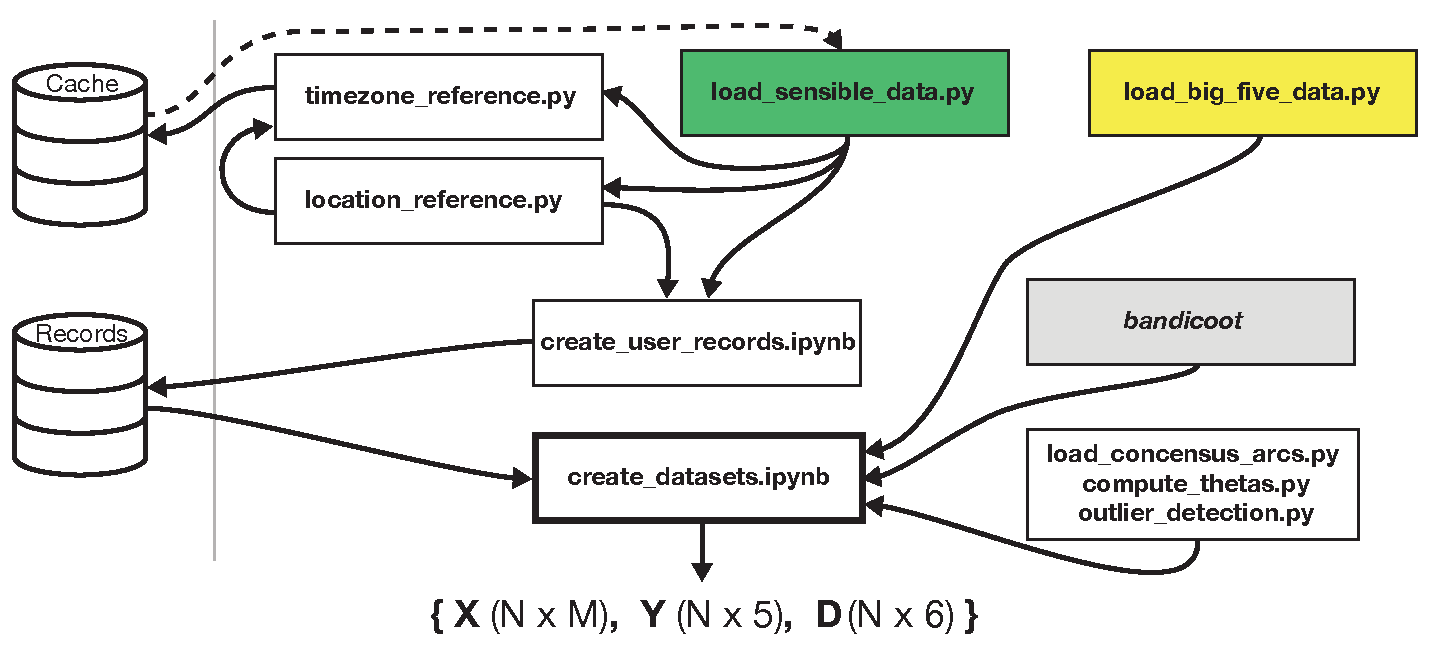
\includegraphics[width=\linewidth]{figures/preprocessing_pipeline}
	\end{minipage}
	\begin{minipage}[r]{0.19\textwidth}
		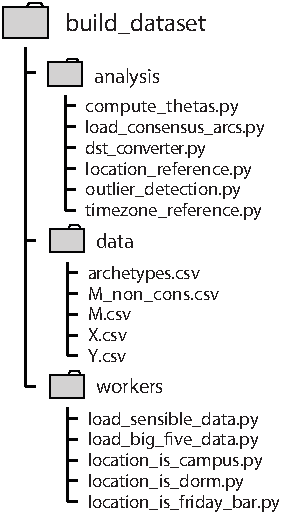
\includegraphics[width=\linewidth]{figures/preprocessing_repo}
	\end{minipage}
	\caption{\label{fig:preprocessing_pipeline}Preprocessing pipeline implemented on the virtual IPython notebook environment (see Sec. \ref{subsec:sensibleDTU}). The researcher first creates records for all users in a format that is accepted by the modified version of bandicoot, then uses bandicoot and pipeline submodules to compute three datamatrices: behavioral indicators $\matr{X}$, Big Five personality traits $\matr{Y}$ and weighted euclidian distances from precomputed consensus archetypes $\matr{D}$.}.
\end{figure}

The analysis pipeline is made available on Github at:\\

\url{https://github.com/ulfaslak/MScProject-build-dataset}

		% Feature Engineering
		\subsubsection{Feature Engineering \label{subsubsec:featureEngineering}}
		Feature engineering is carried out with focus on producing statistically independent behaviroal indicators, such as to capture as much of the behavioral spectrum with as little redundancy as possible. Views on importance of this is discussed in Appendix \ref{app:aNoteOnFeatureEngineering}. For extracting behavioral indicators (herinafter just \textit{indicators}) the Python package \textit{bandicoot} is used, and extended to handle multiple data-types. bandicoot is a call-detail-record (CDR) analysis package that offers phone companies and researchers to extract a comprehensive array of measurements of behavior based on text and call records\mcite{de2013predicting}. It works by loading records for individual users as comma separated values (CSV) which it expects to contain certain attributes such as \texttt{timestamp}, \texttt{interaction}, \texttt{correspondent-id}, into \texttt{Record} objects and creating \texttt{User} objects which contain their \texttt{Records} as parameters as well as other parameters inferred from the loaded records such as \textit{home} if the data contains location labels. The analyst then specifies whether to compute indicators for each day, week or month or the entire period comprising the data, whether to treat day and night or weekdays and weekends separately and finally which indicators to compute. Some of these rely on records being grouped into \textit{conversations} which are defined as dyad exchanges that are not delayed by more than some time constant (typically 30 minutes or 1 hour). Two extensions to bandicoot were made:
\begin{enumerate}
	\item Generalization of the the \texttt{Record} object to be any kind of data which only requires to have \texttt{timestamp} as an attribute.
	\item Modifying existing indicators to accept new data-types and adding new indicators that combine data from multiple channels.
\end{enumerate}
 
An example of (2) is that using multiple data channels allows for creation of indicators that show how much use their phone when they are social (channels: F2F and screen), how much they tend to go in groups rather than be in dyads (time overlap between F2F \textit{conversations}) and whether they tend to socialize with friends from the university \textit{outside of the university} (F2F and stop-locations). A full list of the indicators which are used is shown in Appendix \ref{app:fullListOfExtractedFeatures}, where it is marked which are added for this study and which already exist in the standard bandicoot version. The project code for the standard and extended versions of bandicoot is available, respectively, at:\\

\url{github.com/yvesalexandre/bandicoot}

\url{github.com/ulfaslak/bandicoot}\\

In this study, features were computed across the entire period since it was expected that the filtering criteria explained in Figure \ref{fig:data_activity} would provide sufficient behavioral consistency in the data.

		% Variable Transformation
		\subsubsection{Variable Transformation \label{subsubsec:variableTransformation}}
		Two steps of variable transformation is employed:
\begin{enumerate}
	\item Domain scaling
	\item Form transformation
\end{enumerate}

\textbf{For (1):}
The indicators that the extended version of bandicoot returns are scaled in different domains. Most of them either return ratios or count variables, which can be problematic to analysis methods that are not scaling invariant. To correct for this, the data are structured as a matrix with rows for users and columns for indicators, and the columns are subtracted by their means and divided by their standard deviations such as to enforce zero mean and unit standard deviation for all columns. The same approach is taken for the BF data (but not the distances from consensus archetypes, as this would produce negative distance which confuses the analysis).

\textbf{For (2):}
Some indicators are not normally distributed which can cause problems in analysis because a density shift to one end of the domain can make trends in the data arise although there is none. In most cases, generally, and for all cases in this study, variables that are not normally distributed can be transformed using a scaling function like the logarithmic, square root, square, inverse, etc.. Out of the 38 behavioral indicators used in this study 12 were log-transformed.

		% Outlier Detection
		\subsubsection{Outlier Detection \label{subsubsec:outlierDetection}}
		As Figure \ref{fig:data_activity} shows, the activity of participants in the SensibleDTU study wasn't constant over the entire period, and although care was taken only to use data from the period of most activity (containing 526 participants), all participants cannot be expected to provide useful data that informs the analysis. Therefore two levels of filtering was set up.
The first level of filtering removes outliers using indicator activity thresholds based in careful assumptions about how people use smartphones. The aim is to filter out participants who were not actually using the phone. The assumptions are: (1) not everyone likes calling and texting, but everyone carries their phone with them on most days, (2) average over time people are within 1.5 meters distance of at least three people every day and (3) changes location at least twice daily. These conditions remove 84 participants from the analysis.
The second level of filtering uses kernel density estimation (KDE) for removing outliers\mcite{latecki2007outlier}. It employs a very simple scheme that computes kernel density (KD) (using the Python module \texttt{sklearn}) for each datapoint and removes those that fall below an empirically chosen threshold. This removes 30 participants from the analysis.
After both levels of filtering \textbf{412 valid datapoints remain}.

		% Extracting personality data
		\subsubsection{Personality Data Extraction \label{subsubsec:extractingPersonalityData}}
		The BF personality questionnaire used in the SensibleDTU study is a version of the BF Inventory\mcite{john1999big}, translated from English into Danish. It contains 44 individual items and each BFT is computed as the average of 7-10 items. To extract the traits, reference \cite{facet54big} was used.

	% Analysis
	\subsection{Analysis \label{subsec:methods:analysis}}
	In the following, details about how analysis is conducted, which cannot be understood from Section \ref{sec:results}, is explained. It gives an account of the details which enables others to reproduce, however for very exact details and code (of which this section consciously includes very little), the reader is referred to the Github repository at \cite{projectCode}.

		% Computing consensus archetypes
		\subsubsection{Computing consensus archetypes \label{subsec:computingConsensusArchetypes}}
		Section \ref{subsec:consensusArchetypes} explains that six consensus archetypes are found to emerge across seven datasetets. In the following the methods used to arrive at this result is explained.

Employing archetypal analysis on a for a large number of points prove problematic when the domain is constrained (in this case from [-1 ; 1]), because noise in the data causes all subdomains of the space to fill up. For BF datapoints which exist in five dimensions, the full dataset therefore constitute a 5D cube (a \textti{hypercube}), which leads the archetypes to snap the the vertices of this box. Therefore a different approach is taken. Considering Figure \ref{fig:convexHullCurseOfDimensionality} the convex hull in five dimensions of just 200 points only contains about 20\% of the datapoints in a point cloud. Furthermore, 200 points are found to constitute a small enough subset that points rarely go to the geometrical extremes of the domain. Howver, it is observed that using such a small number of points often leads to archetypes that are very different between iterations, and as such the following approach for finding the archetypes is taken (all references to row sorting use the algorithm shown in Python code in Listing \ref{lst:reorder_to}):

\begin{enumerate}
	\item Compute archetype 5000 times for subsets of 200 points for each of the seven datasets, using Python implementation of AA\mcite{pypcha}. This yields a tensor $\matr{X}$ which has dimensions $(N=6) \times (M=5) \times (K=5000)$, where $N$ are archetypes, $M$ are BFTs and $K$ are iteration slices, indexed $i$, $j$, $k$, respectively (see Figure \ref{fig:entryWiseStatistics}).
	\item For each dataset:
	\begin{enumerate}
		\item For each pair of iteration slices (of which there are $(K-1)^2/2$) sort rows to minimize average distance between points, and record the distance between the pairs. Remove the 50\% of all iteration slices starting with the ones of highest average distance to other slices.
		\item In two-iteration steps, sort rows of $\matr{X}_{k+1}$ with respect to rows of $\matr{X}_{k}$ such as to minimize average distance between archetypes. Replace pair with average along 2nd axis. Repeat until there is only one slice left. This constitutes the archetypes of the dataset.
	\end{enumerate} 
	\item Sort resulting rows for each dataset using one as a reference. This yields the archetypes shown in Figure \ref{fig:medianDistances}. Stack them in depth to form a matrix of shape $6 \times 5 \times 7$ and compute the SD and median matrices along the 2nd axis, $\matr{\Sigma}$ and $\matr{A}$ respectively.
	\item Repeat step (3) 1000 times where columns in each slice are shuffled, and record the distribution of SDs along the 2nd axis. Take the maximum value of the 5th percentile as a threshold, $\lambda$, for maximally allowed SD between archetype traits (consensus threshold, see Figure \ref{fig:varianceThreshold}).
	\item Enforce $\lambda$ on $\matr{\Sigma}$ and apply the resulting mask to $\matr{A}$ to reveal the consensus archetypes.
\end{enumerate}

\begin{figure}
	\centering
	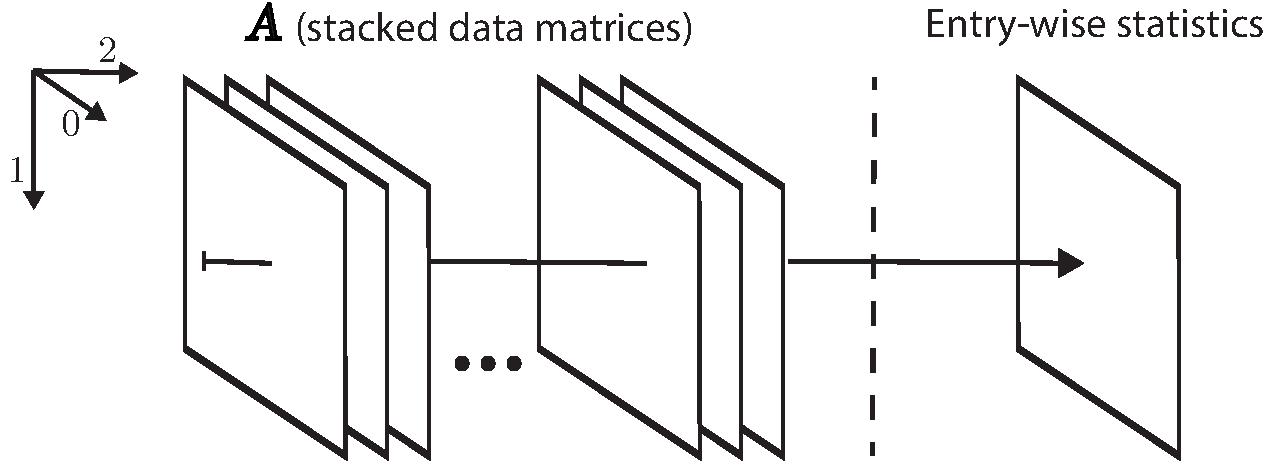
\includegraphics[width=1\textwidth]{figures/entryWiseStatistics}
	\caption{\label{fig:entryWiseStatistics} Example of how 2D matrices are stacked to shape a 3D tensor. The coordinate system explains the use of axis labels in the text, and the 'Entry-wise statistics' matrix illustrates how e.g. SD, mean or median values result from computing such along the 2nd axis.}
\end{figure}

% python code
\definecolor{codegreen}{rgb}{0,0.6,0}
\definecolor{codegray}{rgb}{0.5,0.5,0.5}
\definecolor{codepurple}{rgb}{0.58,0,0.82}
\definecolor{backcolour}{rgb}{0.95,0.95,0.92}
 
\lstdefinestyle{mystyle}{
    backgroundcolor=\color{backcolour},   
    commentstyle=\color{codegreen},
    keywordstyle=\color{magenta},
    numberstyle=\tiny\color{codegray},
    stringstyle=\color{codepurple},
    basicstyle=\footnotesize,
    breakatwhitespace=false,         
    breaklines=true,                 
    captionpos=b,                    
    keepspaces=true,                 
    numbers=left,                    
    numbersep=5pt,                  
    showspaces=false,                
    showstringspaces=false,
    showtabs=false,                  
    tabsize=2
}
 
\lstset{style=mystyle}

\begin{lstlisting}[language=Python, label={lst:reorder_to}, caption="Python code for sorting rows of matrix $\matr{A}$ to match those of $\matr{B}$"]
import numpy as np
def reorder_to(A, B):
    """Return order of rows in A the best match rows in B."""
    distance_matrix = np.ones((6, 6))*np.inf
    for i, a in enumerate(A):
        for ii, b in enumerate(B):
            ba = (b-a)
            distance_matrix[i, ii] = np.sqrt(np.dot(ba, ba))
    reorder = [[] for _ in range(6)]
    for _ in range(6):
        ind = np.argmin(distance_matrix)
        i, ii = ind/6, ind%6
        reorder[ii] = i
        distance_matrix[i, :] = np.inf
        distance_matrix[:, ii] = np.inf
    return reorder
\end{lstlisting}

		% Computing enrichments
		\subsubsection{Computing enrichments \label{subsec:enrichment}}
		For the early research conducted in this project, enrichment was analyzed using the ParTI software package developed by the Uri Alon group\mcite{hart2015inferring}. However as Figure \ref{fig:enrichmentExample} illustrates the concept of enrichment is simple, and as such an implementation was made in Python which is shown in Appendix \ref{app:enrichment_code}. It takes a matrix of precomputed distances between samples and archetypes $\matr{D}$ and a matrix of feature-values corresponding to the same samples, and returns a JSON object that contains enrichments for each feature near each archetype (example given in Appendix \ref{app:enrichment_code}). Standard errors are computed for each associated bin as $\mathrm{SD}/\sqrt{N}$ where $N$ is the number of samples. Since the number of samples is large the standard error goes to 0 and is therefore not shown on the enrichment plots in Figure \ref{fig:firstEnrichmentsQuestionnaireValues}.

Statistical significance of enrichments is computed for the null hypothesis that: \textit{any random permutation of bins will result in greater $R^2$ \textbf{and} slope values for a first order polynomial fitted to the bin values}. The significance level is set to $\alpha = 0.05$ and a Bonferroni multiple hypothesis correction is used\mcite{dunn1961multiple}. For enrichment of attributes and facets, of which there are collectively 780 which all stem from the SAPA dataset, enrichments are therefore only accepted if they have a $p-$value smaller than $\alpha/780$, since there are 780 hypotheses being tested. For BHVs of which there are 10 the threshold is $\alpha/10$.

		% Computing correlations
		\subsubsection{Computing correlations \label{subsec:correlations}}
		For computing linear relationships between behavioral indicator values and distance from archetypes, the Pearson product-moment correlation method is used\mcite{pearson1895note}. It estimates the ratio between the covariance of two variables normalized by the product of their individual variances, and as such does not provide an estimate for the slope of the covariance, only its strength and sign. This is, however, considered valid because the analysis goal is only to find evidence of the existence of relationships and not to model them.

Statistical significance is tested using a permutation test for the null hypothesis that: \textit{randomly redefined coordinate pairs from the original coordinates yields greater correlation coefficients than the original data}. A significance level, $\alpha = 0.05$, is used and a Benjamin-Hochberg (BH) multiple comparisons correction is used. The BH correction is less strict than the Bonferroni correction mentioned in Section \ref{subsec:enrichment} but is widely accepted, especially by those that consider the Bonferroni correction too harsh. It sorts the $p-$values of $N$ tests such that each is denoted $p_i$ and states that in order for a test $i$ to be significant it must obey:

\begin{equation}
	p_i = \frac{\alpha}{N} i
\end{equation}

Any test $i$ which is significant, renders all preceding tests significant also.

		% Classification
		\subsubsection{Classification \label{subsec:classification}}
		It is outside of the scope of this thesis to give an exhaustive account of classification in machine learning and as such no dedicated section to explain this is included in the theory chapter, but for good measure a brief introduction to the subject is given below. Supervised learning constitutes a very rigid analytical paradigm: given a set of \textit{observations} $\matr{X} = [\matr{x}_1, \matr{x}_2, ..., \matr{x}_n]^\top \in \mathbb{R}^{n \times m}$ which has a corresponding set of \textit{labels} $\matr{y} = [\matr{y}_1, \matr{y}_2, ..., \matr{y}_n]^\top \in \mathbb{R}^{n \times 1}$ supervised learning aims to learn the labels that typically result from different types of observations. If the labels for example were "cat" or "dog", and features were "paw size", "body weight", "has whiskers", "barks", a supervised machine learning algorithm would be trained to learn the \textit{decision boundary} that separates the classes and be able to predict whether new unseen data corresponded to a cat or a dog. Modeling is, however, not always the primary concern when applying supervised machine learning. As is the case with the current analysis, it is often desired to get an estimate of the \textit{accuracy} with which a target variable can be predicted from a given type of data. To do this, the orignal dataset $\matr{X}$ is split into a \textit{training fold} $\matr{X_\mathrm{train}}$ and a \textit{test fold} $\matr{X_\mathrm{test}}$. The model is then trained on $\matr{X_\mathrm{train}}$ and the reported accuracy is the percentage of labels it guess correctly when it is tested on $\matr{X_\mathrm{test}}$. This sectioning of training and test data can be done in a variety of ways to get the most information out of the available data. In the current analysis a \textit{cross validation} approach is used for doing this. There exist many different models for classification one of the simplest being \textit{decision trees} that learns to separate data by sequential decision rules which best separates it into different classes. An extension of this model is the \textit{random forest} which trains many trees that in turn "vote" for which class a given sample should belongs to.

Section \ref{subsec:classification} investigates whether consensus archetypes provide better prediction targets than Big Five traits and QI PCs using a supervised machine learning approach. For each target accuracy is reported for a three-class optimized random forest classifier which is validated using a random sampling cross-validation approach (explained below). The optimization scheme optimizes the parameters \texttt{n\_estimators} and \texttt{max\_features} which are generally considered the most important parameters to tune for random forest models\mcite{sklearnEnsemble}. \texttt{n\_estimators} decides the number of trees which the forest model trains and uses for voting, and \texttt{max\_features} is the maximal number of randomly selected features which are considered at each split. The scheme works in two steps: (1) estimate validation scores 100 times for random parameter settings and record the parameter combination $(p_1^{opt},p_2^{opt})$ which lead to the highest score, then (2) do a $10 \times 10$ grid-search in the quadratic range of $[p_1^{opt}-\frac{p_1^{opt}}{2}; p_1^{opt}+\frac{p_1^{opt}}{2}]$ and $[p_2^{opt}-\frac{p_2^{opt}}{2}; p_2^{opt}+\frac{p_2^{opt}}{2}]$ to find the optimal parameters.

Cross-validation is performed over 100 folds. In each fold the model is trained on a subset of 80\% randomly selected samples from the dataset and tested on the remaining 20\%. The reported accuracy is the average of this. SD of acuracies across folds are around 2\% so for 100 fold the standard error evaluates to around 0.2\%.

% \begin{figure}
% 	\centering
% 	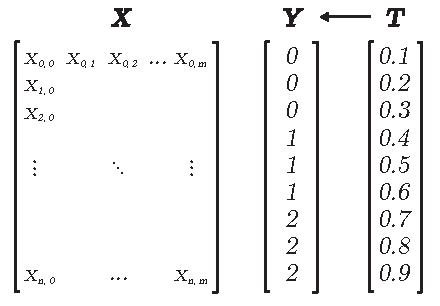
\includegraphics[width=0.5\textwidth]{figures/learningParadigm}
% 	\caption{\label{fig:learningParadigm} Example of how three classes are computed a continuous variable $\matr{T}$. $\matr{Y}$ is the vector of classes that the model learns using data-samples $\matr{X}$.}
% \end{figure}


% References
% ----------
\newpage
\thispagestyle{plain}
\addcontentsline{toc}{section}{References}
\bibliography{includes/bib}


% Appendices
% ----------
\appendix
\newpage
\appendixpage

\noappendicestocpagenum
\addappheadtotoc

% Full List of Extracted Indicators
\section{Full List of Extracted Indicators \label{app:fullListOfExtractedFeatures}}
\thispagestyle{plain}
Complete list of features extracted from the data and used in the analsis, including explanations. Features may be extracted from the sources \texttt{\small call}, \texttt{\small text}, \texttt{\small F2F}, \texttt{\small screen}, \texttt{\small stop}, either solely, or as combinations utilizing the interaction between measurements. Below, feature names are highlighted in bold, and the types used for each feature is listed in brackets: \texttt{\small []}. A bracket in a bracket signifies that the feature is computed from the combination of the datatypes listed in the bracket. A short examplary explanation is given for the first feature. Furthermore features are either computed as \textit{summary} type which yields mean and standard deviation of a distribution, or as \textit{scalar} type yielding a scalar. \textbf{Id} and \textbf{Data} are consistent with function and datatype names in project code. Asterisk '*' marks that the indicator is only a part of the extended bandicoot version, however note that most of the standard indicators have also been extended to accept new data-types.

\subparagraph*{Number of contacts}
Number of individuals interacted with. Requires more than one meeting for an individual to count. Is computed for \texttt{\small text} and \texttt{\small call} (together) and \texttt{\small stop}, resulting in two measures of \textit{number of contacts}. For \texttt{\small stop} it simply measures the number of different places an individual goes. This feature captures the size of an individuals social circle. \texttt{\small F2F} is not included because correspondent Ids are inconsistent for non-study-participant correspondents.\\ \textit{\textbf{Id}: number\_of\_contacts \textbf{Data}: [[\texttt{\footnotesize text}, \texttt{\footnotesize call}], \texttt{\footnotesize stop}] \textbf{Type}: scalar}.

\subparagraph*{Number of interactions}
Number of interaction made. \\ \textit{\textbf{Id}: number\_of\_interactions \textbf{Data}: [[\texttt{\footnotesize text}, \texttt{\footnotesize call}], \texttt{\footnotesize F2F}, \texttt{\footnotesize stop}] \textbf{Type}: scalar}.

\subparagraph*{Ratio of call traffic and text traffic*}
Number of calls made divided by number of texts sent.\\ \textit{\textbf{Id}: ratio\_call\_text \textbf{Data}: [[\texttt{\footnotesize text}, \texttt{\footnotesize call}]] \textbf{Type}: scalar}.

%\subparagraph*{Interaction concentration}
%Percent of contacts that account for 80\% of interactions. Takes basis in the 80/20 "Pareto" principle. For \texttt{\small text} and \texttt{\small call} together, this is computed over conversations.\\ \textit{\textbf{Id}: percent\_ei\_percent\_interactions \textbf{Data}: [[\texttt{\footnotesize text}, \texttt{\footnotesize call}], \texttt{\footnotesize F2F}] \textbf{Type}: scalar}.

\subparagraph*{Duration concentration}
Percent of interactions that account for 80\% of interaction duration. Takes basis in the 80/20 "Pareto" principle. \\ \textit{\textbf{Id}: percent\_ei\_percent\_durations \textbf{Data}: [\texttt{\footnotesize stop}] \textbf{Type}: scalar}.

\subparagraph*{Balance of interactions}
Percent of interactions directed outwards. \\ \textit{\textbf{Id}: balance\_of\_interactions \textbf{Data}: [\texttt{\footnotesize text}] \textbf{Type}: scalar}.

\subparagraph*{Duration}
Duration of interaction. If datatype has a \texttt{\small duration}-attribute (\texttt{\small call}, \texttt{\small screen}, \texttt{\small stop}), this is used, otherwise interactions are grouped into conversations, i.e. series of breaks no longer than one hour, and the duration of these are used to compute average duration.
\\ \textit{\textbf{Id}: duration \textbf{Data}: [\texttt{\footnotesize call}, \texttt{\footnotesize text}, \texttt{\footnotesize F2F}, \texttt{\footnotesize screen}, \texttt{\footnotesize stop}] \textbf{Type}: scalar}.

\subparagraph*{Percent initiated conversations}
Percent conversations initiated. Conversations are inferred from series of interactions grouped by correspondent, as clusters with no more than one hour long breaks. Standard deviation across percent initiated for set of correspondents, yielding standard deviation a measure of "selectiveness" in who the individual chooses to initiate interaction with. For \texttt{\small call}, an outgoing missed \texttt{\small call} counts as an initiated conversation, whereas an incoming missed \texttt{\small call}, even though returned, does not.\\ \textit{\textbf{Id}: percent\_initiated\_conversations \textbf{Data}: [\texttt{\footnotesize text}, \texttt{\footnotesize call}] \textbf{Type}: summary}.

\subparagraph*{Percent concluded conversations*}
Similar to 'Percent initiated conversations' but for last interaction in conversation, i.e. \textit{conclusion}. Call is not used because it produces no informative feature.\\ \textit{\textbf{Id}: percent\_concluded\_conversations \textbf{Data}: [\texttt{\footnotesize text}] \textbf{Type}: summary}.

\subparagraph*{Response delay}
Response delay in conversations grouped by correspondents. Maximum delay is one hour.\\ \textit{\textbf{Id}: response\_delay \textbf{Data}: [\texttt{\footnotesize call}, \texttt{\footnotesize text}] \textbf{Type}: summary}.

\subparagraph*{Response rate}
Response rate to conversations initiated by correspondents, grouped by correspondent. Response counts if returned within the first hour, otherwise it counts as a delay.\\ \textit{\textbf{Id}: response\_rate \textbf{Data}: [[\texttt{\footnotesize call}, \texttt{\footnotesize text}]] \textbf{Type}: summary}.

\subparagraph*{Overlap of social meetings*}
Proportional to average number of people together with when social. Computed from overlap of conversations. Captures propensity to go in groups.\\ \textit{\textbf{Id}: overlap\_conversations \textbf{Data}: [\texttt{\footnotesize F2F}] \textbf{Type}: scalar}.

\subparagraph*{Percent nocturnal}
Percent of activity that occurs between 22pm and 6am.\\ \textit{\textbf{Id}: percent\_nocturnal \textbf{Data}: [\texttt{\footnotesize F2F}, \texttt{\footnotesize screen}, \texttt{\footnotesize stop}] \textbf{Type}: scalar}.

\subparagraph*{Interevent time}
Average time between events. For screen this captures the average time between phone usage sessions.\\ \textit{\textbf{Id}: ratio \textbf{Data}: [\texttt{\footnotesize screen}] \textbf{Type}: scalar}.

\subparagraph*{Phone use while social*}
Amount of phone use while social divided by amount of phone use while alone.\\ \textit{\textbf{Id}: ratio\_social\_screen\_alone\_screen \textbf{Data}: [[\texttt{\footnotesize screen}, \texttt{\footnotesize F2F}]] \textbf{Type}: scalar}.

\subparagraph*{Ratio of interactions at campus vs. elsewhere*}
No. interactions that occur within campus regions divided by no. interactions that occur outside of campus and inferred home regions.\\ \textit{\textbf{Id}: ratio\_interactions\_campus\_other \textbf{Data}: [[\texttt{\footnotesize stop}, \texttt{\footnotesize F2F}]] \textbf{Type}: scalar}.

\subparagraph*{Percent interactions elsewhere with people from campus*}
Percent of all interactions that occur outside campus, dorms and inferred home regions, which are made with individuals that were also interacted with at campus. Captures level of non-curricular social engagement with school mates. Excludes home because a large group of study participants live at campus dorms, and would exhibit far greater values in this feature for reasons not necessarily related to social engagement.\\ \textit{\textbf{Id}: percent\_outside\_campus\_from\_campus \textbf{Data}: [[\texttt{\footnotesize stop}, \texttt{\footnotesize F2F}]] \textbf{Type}: scalar}.

\subparagraph*{Percent daily time at campus*}
Average percent of all daily time (24 h) spent at campus.\\ \textit{\textbf{Id}: percent\_at\_campus \textbf{Data}: [\texttt{\footnotesize stop}] \textbf{Type}: scalar}.

\subparagraph*{Daily average number of stranger interactions*}
Percentage of \texttt{\small F2F} conversations, i.e. connections grouped into series of less than 24 hour breaks, that occur only once. Captures an individuals propensity to engage in social activities with people outside of their social circle, such as talking with people in bars, or joining a group of mixed friends for a weekend in a summer house. May include some noise from non-social connections made in transportation and other public spaces.\\ \textit{\textbf{Id}: number\_of\_contacts\_less \textbf{Data}: [\texttt{\footnotesize F2F}] \textbf{Type}: scalar}.

\subparagraph*{First seen response rate*}
Percent of texts that are responded to during first possible session, i.e. right away when observed by the individual.\\ \textit{\textbf{Id}: first\_seen\_response\_rate \textbf{Data}: [[\texttt{\footnotesize screen}, \texttt{\footnotesize text}]] \textbf{Type}: scalar}.

\subparagraph*{Interaction autocorrelation*}
Average autocorrelation of \texttt{\small F2F} togetherness across an individuals dyadic relationships. Captures a facet of the kind of relationships an individual maintains, where a high value means that most relationships fit into a schedule and are non-spontaneous and low values means most meetings are improptu. Only includes dyads that are observed in conversation more than 5 times.\\ \textit{\textbf{Id}: interaction\_autocorrelation \textbf{Data}: [\texttt{\footnotesize F2F}] \textbf{Type}: scalar}.
\newpage

% A Note on Feature Engineering
\section{A Note on Feature Engineering \label{app:aNoteOnFeatureEngineering}}
\thispagestyle{plain}
An important notion to introduce when processing data and designing features for use in machine learning or signal processing, is that the amount of information, or entropy, contained in a data source depends not only on its size but also on the presence of patterns such as mutual information between latent variables and periodicity in series. In the present \textit{Big Data} context this rarely enters as a problem of information scarcity, but rather as a source of error due to the risk of capturing uninformative patterns in the feature design, which may go unobserved thus leading to false conclusions. To give an intuition of how this can cause problems, consider the following example.\\

\texttt{feature A} measures the fraction of time a user is looking at his or her phone while socially engaged, and \texttt{feature B} measures the unique number of friends that the user has through a given period. If one were to plot the distribution of these variables for a set of individuals against eachother, it would yield an almost perfect inverse correlation, begging the interpretation that looking at your phone while socially engaged means you have less friends. The problem with this analysis is that \texttt{feature A} is normalized by the summed time socially engaged, which unsurprisingly correlates with \texttt{feature B}. The consequence is that the latent variable the analyst is trying to get at, namely the propensity to interact with one's phone while social, vanishes in product with a variable that so strongly correlates with the target. At the same time, removing the normalization term creates the inverse problem, because the summed time of phone use while socially engaged necessarily depends on how much a user engages socially and thereby number of unique friends. In the given case, a better design of \texttt{feature A} would be to measure the \textit{amount of phone use while socially engaged vs. while alone} in which case it should behave independently from other features.\\

Uninformative patterns are expected for mathematical, systematic or other boring reasons, and are often undesired since they wash out interesting informative patterns, like in the example given above. Patterns which are considered most informative are those that emerge unexpectedly or in line with a hypothesis and demands explanation only through interpretation or further research. In general, careful consideration must be made to capture mostly patterns that informs the analysis. Features must be designed to cultivate patterns that express properties of the system which are not entirely self-evident. This excludes not only features capturing uninformative patterns, but also a large number of other features we as humans know to be mutually informative or in correlation. Consider how, for a set of individuals, the \textit{number of calls made} vs. \textit{number of calls received} would, aligned with our expectations, be in strong correlation, but that \textit{number of calls made and received} vs. \textit{percent of calls going out}, would not. Both feature pairs are derived from the same call-log data, but as illustrated in Fig. \ref{fig:example_informative_features}, a far more informative pattern is captured with the latter pair.

\begin{figure}[h!]
	\centering
	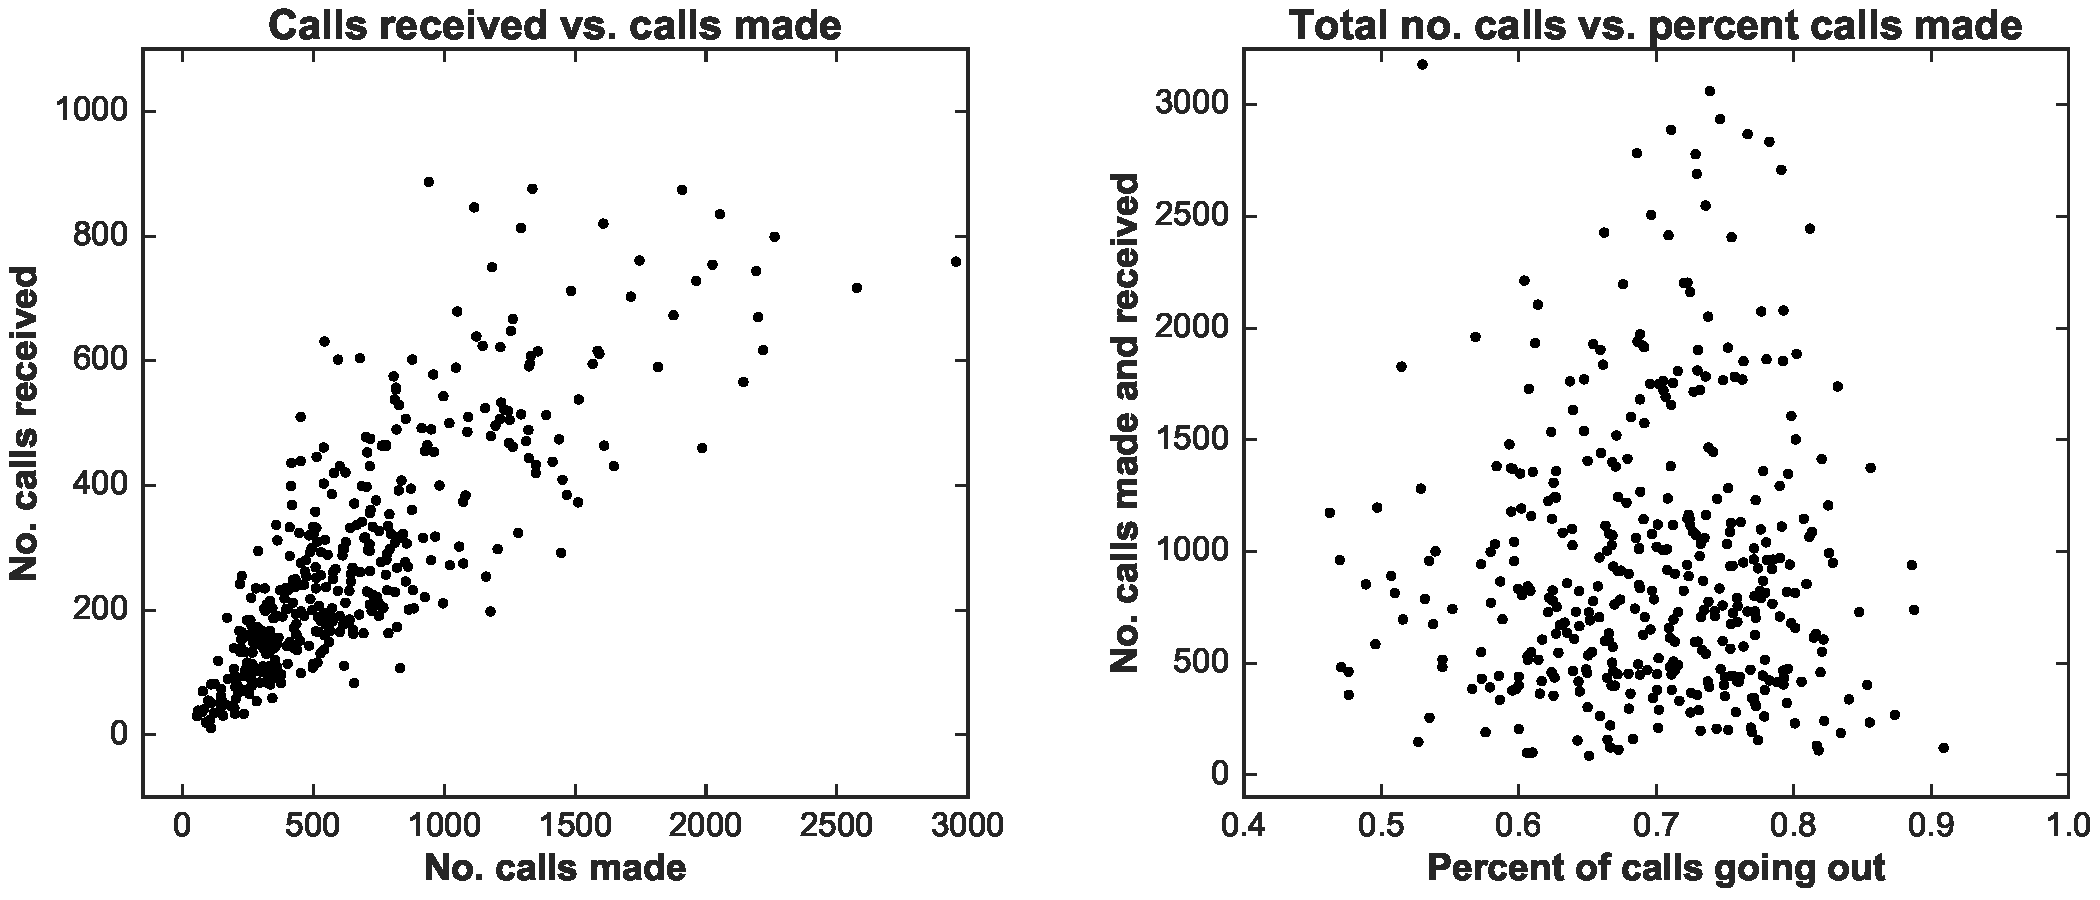
\includegraphics[width=0.9\textwidth]{figures/example_informative_features}
	\caption{\label{fig:example_informative_features} Casting features differently changes the pattern they capture. Each plot represents a different way of casting the same call-log data, but the right one obviously captures a more informative pattern. It allows one to make genuinely interesting observations, such as how only individuals with an outgoing to incoming call ratio between 0.7 and 0.8 make and receive far above average number of calls.}
\end{figure}

In practice it is tedious to engineer features to only capture patterns that inform the analysis. In fact, trying to achieve this often creates problems since the task of developing the necessary complex features requires significantly more coding, which increases the risk of generating uncaught bugs. In this work, it is attempted to strike a balance between the informative and the simple. In other words, great care has been taken to understand the data which has led to the realization that it is not feasible to completely avoid capturing uninformative patterns, and as such features are designed in a way that attempts to minimize these, not exclude them.
\newpage

% Questionnaire Enrichment Table
\section{Questionnaire Enrichment Table \label{app:questionnaireEnrichmentTable}}
\thispagestyle{plain}
Slopes of enrichment curves for Big Five questionnaire items near consensus personality archetypes. Negative slope indicate enrichment and positive slope indicate depletion. * denotes statistical significance after Bonferroni correction.\\

%\newenvironment{allintypewriter}{\ttfamily}{\par}
\newcommand{\mcc}[1]{\multicolumn{1}{R{1.3cm}}{#1}}

{
\centering
\footnotesize
\hspace{-2cm}
\begin{tabular}{rrrrrrr}
\toprule
{} 				& \mcc{\smallachiever} 		& \mcc{\smallhost} 			& \mcc{\smallwildcard} & \mcc{\smallloyalist} 		& \mcc{\smallhippie} 			&  \mcc{\smallfollower} \\
\midrule
Get overwhelmed by emotions [N]                           & \textbf{0.114}* &-0.099* & 0.091* &-0.0249 & 0.0762 &-0.110*\\
Indifferent to others' emotions [!A]             &\textbf{-0.112}* & 0.0374 & 0.0588 & 0.0266 &-0.0205 &-0.0121\\
Have a soft heart [A]                                     & \textbf{0.109}* &-0.0426 &-0.0423 &-0.0326 & 0.0428 &-0.0023\\
Am out for my own personal gain [!A]                      &\textbf{-0.107}* & 0.0068 & 0.0541 & 0.0306 &-0.0217 & 0.0028\\
Believe that I am better than others [!A]                 &\textbf{-0.102}* &-0.0109 & 0.0395 & 0.0518 &-0.0178 & 0.0010\\
Feel others' emotions [A]                                 & \textbf{0.101}* &-0.0604 &-0.0593 &-0.0211 & 0.0316 & 0.0128\\
My feelings are easily hurt [N]                           & \textbf{0.100}* &-0.085* & 0.084* &-0.0273 & 0.0696 &-0.097*\\
Am sensitive to the needs of others [A]                   & \textbf{0.100}* &-0.0416 &-0.0612 &-0.0209 & 0.0303 & 0.0197\\
Use others for my own ends [!A]                           &\textbf{-0.098}* & 0.0002 & 0.0544 & 0.0407 &-0.0310 &-0.0015\\
Take advantage of others [!A]                             &\textbf{-0.094}* &-0.0090 & 0.0604 & 0.0273 &-0.0234 &-0.0200\\
Look down on others [!A]                                  &\textbf{-0.087}* &-0.0058 & 0.0728 & 0.0297 &-0.0097 &-0.0353\\
Inquire about others' well-being [A]                      & \textbf{0.084}* &-0.0543 &-0.0698 &-0.0131 & 0.0201 & 0.0383\\
Am a talkative person [E]                                 & 0.0287 &\textbf{-0.153}* &-0.094* & 0.0260 & 0.0006 & 0.123*\\
Can be stirred up easily [N]                              & 0.0587 &\textbf{-0.095}* & 0.0705 &-0.0119 & 0.0667 &-0.0730\\
Need reassurance [N]                                      & 0.0660 &\textbf{-0.082}* & 0.0707 &-0.0227 & 0.0445 &-0.0766\\
Am often down in the dumps [N]                            & 0.0656 &-0.0440 & \textbf{0.142}* & 0.0069 & 0.0516 &-0.139*\\
Do too little work [!C]                                   & 0.0116 & 0.0007 & \textbf{0.112}* & 0.0347 &-0.099* &-0.0452\\
Find it difficult to get down to work [!C]                & 0.0272 &-0.0158 & \textbf{0.107}* & 0.0294 &-0.090* &-0.0537\\
Waste my time [!C]                                        & 0.0167 &-0.0077 & \textbf{0.102}* & 0.0236 &-0.0753 &-0.0543\\
Neglect my duties [!C]                                    & 0.0131 &-0.0105 & \textbf{0.098}* & 0.0290 &-0.089* &-0.0398\\
Get easily agitated [N]                                   & 0.0418 &-0.0729 & \textbf{0.098}* &-0.0121 & 0.0591 &-0.095*\\
Make careless mistakes [!C]                               & 0.0193 &-0.0305 & \textbf{0.088}* & 0.0200 &-0.0661 &-0.0331\\
Feel that most people can't be trusted [!A]               &-0.0599 & 0.0053 & \textbf{0.078}* & 0.0155 & 0.0233 &-0.0559\\
Need a creative outlet [O]                                & 0.0158 &-0.0406 &-0.0035 & \textbf{0.101}* &-0.0245 &-0.0123\\
Am not interested in abstract ideas [!O]                  & 0.0094 & 0.0062 & 0.0170 &\textbf{-0.098}* & 0.0339 & 0.0063\\
Know the answers to many questions [O]                    &-0.0270 &-0.0159 &-0.0400 & \textbf{0.098}* &-0.0207 & 0.0296\\
Am full of ideas [O]                                      &-0.0042 &-0.0331 &-0.0346 & \textbf{0.096}* &-0.0156 & 0.0201\\
Have a rich vocabulary [O]                                &-0.0085 &-0.0175 &-0.0268 & \textbf{0.094}* &-0.0226 & 0.0128\\
Have a vivid imagination [O]                              & 0.0024 &-0.0312 &-0.0154 & \textbf{0.087}* &-0.0193 &-0.0021\\
Can handle complex problems [O]                           &-0.0258 &-0.0088 &-0.0444 & \textbf{0.086}* &-0.0144 & 0.0214\\
Complete my duties as soon as possible [C]                &-0.0036 &-0.0034 &-0.087* &-0.0349 & \textbf{0.112}* & 0.0349\\
Keep things tidy [C]                                      &-0.0224 &-0.0002 &-0.0732 &-0.0417 & \textbf{0.102}* & 0.0244\\
Start tasks right away [C]                                &-0.0149 &-0.0109 &-0.091* &-0.0154 & \textbf{0.099}* & 0.0442\\
Stick to the rules [C]                                    & 0.0167 & 0.0063 &-0.0424 &-0.0633 & \textbf{0.099}* &-0.0104\\
Do things by the book [C]                                 &-0.0101 & 0.0236 &-0.0314 &-0.0577 & \textbf{0.093}* &-0.0215\\
Like order [C]                                            &-0.0049 &-0.0028 &-0.0369 &-0.0352 & \textbf{0.089}* &-0.0072\\
Do things according to a plan [C]                         &-0.0152 & 0.0005 &-0.0547 &-0.0295 & \textbf{0.088}* & 0.0086\\
Talk to many diff. people at parties [E]          		  & 0.0119 &-0.137* &-0.123* & 0.0086 &-0.0103 & \textbf{0.153}*\\
Enjoy interactions less than others [!E]                  &-0.0373 & 0.122* & 0.128* & 0.0206 &-0.0036 &\textbf{-0.148}*\\
Make friends easily [E]                                   & 0.0234 &-0.117* &-0.124* &-0.0009 & 0.0009 & \textbf{0.146}*\\
Keep in background on social occasions [!E]   		  &-0.0080 & 0.121* & 0.105* &-0.0023 & 0.0237 &\textbf{-0.144}*\\
Can easily get some life into a dull party [E]            & 0.0043 &-0.126* &-0.110* & 0.0262 &-0.0086 & \textbf{0.141}*\\
Prefer reading to meeting people [!E]                     &-0.0099 & 0.102* & 0.099* & 0.0296 & 0.0027 &\textbf{-0.137}*\\
Am mostly quiet when with other people [!E]               &-0.0084 & 0.126* & 0.103* &-0.0052 & 0.0070 &\textbf{-0.135}*\\
Start conversations [E]                                   & 0.0146 &-0.116* &-0.119* & 0.0125 & 0.0072 & \textbf{0.135}*\\
Moods go up and down easily [N]         				  & 0.0642 &-0.088* & 0.130* & 0.0022 & 0.0515 &\textbf{-0.132}*\\
Like mixing with people [E]                               & 0.0258 &-0.121* &-0.113* &-0.0050 &-0.0105 & \textbf{0.132}*\\
Am a worrier [N]                                          & 0.0777 &-0.0634 & 0.088* &-0.0337 & 0.094* &\textbf{-0.126}*\\
Enjoy meeting new people [E]                              & 0.0260 &-0.109* &-0.102* & 0.0106 &-0.0122 & \textbf{0.120}*\\
Panic easily [N]                                          & 0.081* &-0.0641 & 0.108* &-0.0251 & 0.080* &\textbf{-0.117}*\\
Get upset easily [N]                                      & 0.0618 &-0.083* & 0.098* &-0.0234 & 0.080* &\textbf{-0.110}*\\
Am rather lively [E]                                      & 0.0210 &-0.090* &-0.093* & 0.0150 &-0.0040 & \textbf{0.108}*\\
Get caught up in my problems [N]                          & 0.0582 &-0.0622 & 0.094* & 0.0073 & 0.0450 &\textbf{-0.099}*\\
\bottomrule
\end{tabular}
}
\newpage

% Basic Human Values Enrichment Table
\section{Basic Human Values Enrichment Table \label{app:valuesEnrichmentTable}}
\thispagestyle{plain}
Slopes of enrichment curves for Basic Human Values near consensus personality archetypes. Negative slope indicate enrichment and positive slope indicate depletion. * denotes statistical significance after Bonferroni correction.\\\\

%\newenvironment{allintypewriter}{\ttfamily}{\par}

{
\centering
\footnotesize
\begin{tabular}{lrrrrrr}
\toprule
{} 					& \smallachiever 	& \smallhost 		& \smallwildcard & \smallloyalist & \smallhippie 	&  \smallfollower \\
\midrule
Power	 			& \textbf{-0.030}* 	& -0.013* 			& -0.0008 	& -0.0048 			&  0.013* 			&  0.010* \\
Benevolence	 		& \textbf{ 0.021}* 	& -0.0043 			& -0.020* 	& -0.0043 			&  0.009* 			&  0.007* \\
Hedonism	 		& -0.008* 			& \textbf{-0.016}* 	& -0.0004 	&  0.013* 			& -0.006* 			&  0.006* \\
Self-Direction		& -0.0049 			& -0.0068 			& -0.0074 	& \textbf{ 0.026}* 	& -0.0017 			&  0.0025 \\
Conformity	 		&  0.014* 			&  0.001* 			& -0.023* 	& \textbf{-0.024}* 	&  0.023* 			&  0.011* \\
Tradition	 		&  0.014* 			&  0.0037 			& -0.014* 	& \textbf{-0.021}* 	&  0.010* 			&  0.004* \\
Universalism 		&  0.012* 			& -0.008* 			& -0.012* 	& \textbf{ 0.017}* 	& -0.0002 			&  0.0014 \\
Security	 		&  0.0003 			& -0.004* 			& -0.012* 	& -0.015* 			&  \textbf{0.020}* &  0.008* \\
Achievement	 		& -0.011* 			& -0.010* 			& -0.017* 	&  0.0075 			&  \textbf{0.018}* &  0.012* \\
Stimulation	 		& -0.011* 			& -0.017* 			& -0.018* 	&  0.022* 			& -0.007* 			&  \textbf{0.024}* \\
\bottomrule
\end{tabular}
}
\newpage

% Behavior Correlation Table
\section{Behavior Correlation Table \label{app:behaviorCorrelationTable}}
\thispagestyle{plain}
Correlation coefficients between distance from CAs and behavioral indicators. * denotes statistical significance after Bonferroni correction.\\

%\newenvironment{allintypewriter}{\ttfamily}{\par}

\newcommand{\mcc}[1]{\multicolumn{1}{R{1.5cm}}{#1}}

{
\footnotesize
\hspace{-2cm}
\begin{tabular}{rrrrrrr}
\toprule
{} &         							  \mcc{\achiever} 		& \mcc{\host} 			& \mcc{\wildcard} 		& \mcc{\loyalist} 		& \mcc{\hippie} 		& \mcc{\follower} 	\\
\midrule
Response time to missed calls SD 		& -0.074837				& -0.018582 			& -0.032529 			&  0.055680 			& -0.045662 			&  0.062105 		\\
Frequently calls and texts              &  0.035789				& \textbf{-0.21798*} 	& -0.13202* 			& -0.058639 			&  0.069914 			&  0.13381* 		\\
Has many phone contacts                 &  0.024015				& \textbf{-0.20536*} 	& -0.091237 			&  0.026240 			& -0.017387 			&  0.10454* 		\\
Visits many places only once            & -0.060862				& \textbf{-0.18401*} 	& -0.065878 			&  0.073681 			& -0.080670 			&  0.062021 		\\
Initiates most phone conversations      & -0.014207				& \textbf{-0.17718*} 	&  0.006292 			&  0.005671 			&  0.088067 			& -0.061423 		\\
Goes places often                       & -0.010255				& \textbf{-0.14687*} 	& -0.066594 			& -0.084382 			&  0.080784 			&  0.058721 		\\
Visits many different places            &  0.038093				& \textbf{-0.14040*} 	& -0.099973 			&  0.073829 			& -0.035228 			&  0.039980 		\\
Concludes text conversations            & -0.009717				& \textbf{-0.13497*} 	& -0.10267* 			& -0.080921 			&  0.11701* 			&  0.062394 		\\
Initiates most text conversations       & -0.017914				& \textbf{-0.12941*} 	& -0.044484 			& -0.035294 			&  0.086148 			&  0.009535 		\\
Getting final word when texting SD 		& -0.054429				& \textbf{-0.12736*} 	& -0.048257 			&  0.085706 			& -0.036519 			&  0.071641 		\\
Spends short time at locations          & -0.013552				& \textbf{-0.12319*} 	& -0.10799* 			& -0.077596 			&  0.055401 			&  0.076301 		\\
Calls some people more than others      & -0.061514				& \textbf{ 0.11050*} 	&  0.013780 			&  0.017749 			& -0.062601 			&  0.030792 		\\
Selective text and call response rate   & -0.065717				& \textbf{-0.10107*} 	& -0.078203 			& -0.039442 			&  0.068964 			&  0.040896 		\\
Spends long time with people            &  0.022206				& \textbf{-0.099960} 	&  0.044219 			&  0.015243 			&  0.070682 			& -0.059171 		\\
Around people a lot                     &  0.009494				& \textbf{-0.088931} 	& -0.051458 			& -0.010177 			&  0.053433 			&  0.037501 		\\
Mostly goes in groups                   &  0.000515				& -0.013708 			& \textbf{-0.028966} 	&  0.015795 			&  0.023216 			& -0.021529 		\\
Conversation initiation rate SD    		& -0.039325				& -0.063217 			&  0.009150 			& \textbf{ 0.14673*} 	& -0.081758 			& -0.001845 		\\
Returns calls and responds to texts     & -0.011807				& -0.048248 			& -0.082415 			& \textbf{-0.12769*} 	&  0.10628* 			&  0.072745 		\\
Has long ongoing text conversations     &  0.045167				& -0.030086 			& -0.053182 			& \textbf{-0.10949*} 	&  0.061144 			&  0.022334 		\\
Responds quickly to texts               & -0.022331				&  0.092948 			&  0.028020 			& \textbf{-0.093492} 	&  0.022025 			&  0.031446 		\\
Response time to texts SD 	         	& -0.027276				& -0.025059 			& -0.007418 			& \textbf{ 0.084515} 	& -0.052311 			&  0.013118 		\\
Spends time at campus                   &  0.020200				& -0.045188 			&  0.015450 			& \textbf{-0.082320} 	&  0.053027 			& -0.019011 		\\
Keeps phone sessions short              & -0.017042				&  0.003843 			& -0.021614 			& \textbf{-0.073513} 	&  0.036846 			&  0.026214 		\\
Makes long calls                        &  0.037902				& -0.10913* 			& -0.009160 			& -0.018521 			& \textbf{ 0.19279*} 	& -0.085181 		\\
Meets with people in weekly patterns    &  0.019674				&  0.090653 			&  0.11266* 			& -0.15568* 			& \textbf{ 0.18400*} 	& -0.14523* 		\\
Sends more texts than receives          &  0.001931				& -0.12455* 			& -0.041272 			& -0.052693 			& \textbf{ 0.16598*} 	& -0.019525 		\\
Interacts with strangers                &  0.009526				& -0.030696 			& -0.005149 			&  0.048621 			& \textbf{-0.15726*} 	&  0.051560 		\\
Uses phone at night                     &  0.002887				&  0.049914 			& -0.025226 			&  0.053391 			& \textbf{-0.14350*} 	&  0.045076 		\\
Responds to texts immediately           & -0.024757				&  0.042422 			& -0.090559 			& -0.081023 			& \textbf{ 0.11332*} 	&  0.064325 		\\
Avoids looking at phone when social     &  0.018779				& -0.006039 			& -0.057113 			& -0.007475 			& \textbf{ 0.094036} 	&  0.015023 		\\
Prefers calling over texting            & -0.033625				& -0.014632 			&  0.077649 			&  0.075592 			& \textbf{-0.084600} 	& -0.052389 		\\
Mostly meets people at campus           & -0.079546				&  0.018802 			&  0.14031* 			& -0.035004 			&  0.044647 			& \textbf{0.21230*} \\
Goes many places at night               &  0.004259				&  0.008385 			& -0.11848* 			&  0.076401 			& -0.14232* 			& \textbf{0.18953*} \\
Meets people at night                   &  0.074257				& -0.11076* 			& -0.084527 			&  0.075370 			& -0.10698* 			& \textbf{0.12540*} \\
Doesnt look at phone too often          &  0.028191				&  0.10047* 			&  0.083603 			&  0.10003* 			& -0.046390 			& \textbf{0.11075*} \\
Even time-location distribution      	&  0.001487				& -0.064028 			& -0.069595 			&  0.027634 			& -0.000840 			& \textbf{0.10922*} \\
Meets people from uni. outside uni.	    &  0.055556				& -0.017454 			& -0.044660 			& -0.040767 			& -0.024956 			& \textbf{0.074052} \\
Responds quickly to missed calls        & -0.012016				& -0.023555 			& -0.036409 			&  0.041238 			&  0.020437 			& \textbf{0.051917} \\
\bottomrule
\end{tabular}
}
\newpage

% Theory of Basic Human Values
\section{Theory of Basic Human Values \label{app:theoryOfBasicHumanValues}}
\thispagestyle{plain}
\begin{figure}[!ht]
	\centering
	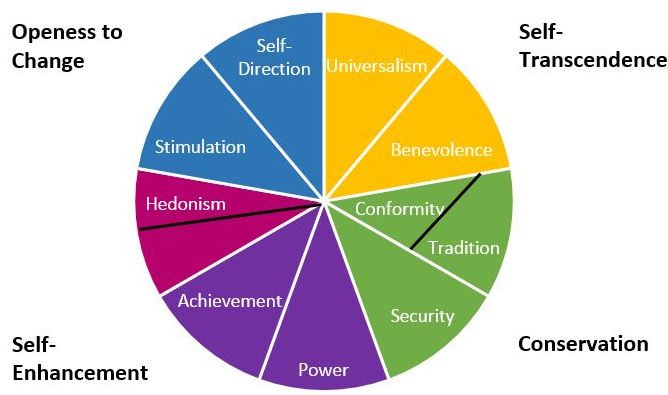
\includegraphics[width=0.7\textwidth]{figures/basicHumanValues}
\end{figure}
\vspace{1cm}
{
\small
\begin{tabular}{ccc}

\textbf{Self-direction}	&	\textbf{Power}					&	\textbf{Spirituality}	\\
Freedom					&	Social power					&	A spiritual life	\\
Creativity				&	Wealth							&	Meaning in life	\\
Independent				&	Authority						&	Inner harmony	\\
Choosing own goals		&	Preserving my public image		&	Detachment	\\
curious					&	Social recognition				&	{}	\\
Self-respect			&	{}								&	\textbf{Benevolence}	\\
{}						&	\textbf{Security}				&	Helpful	\\
\textbf{Stimulation}	&	National security				&	Responsible	\\
An exciting life		&	Reciprocation of favors			&	Forgiving	\\
A varied life			&	Family security					&	Honest	\\
Daring					&	Sense of belonging				&	Loyal	\\
{}						&	Social order					&	Mature love	\\
\textbf{Hedonism}		&	Healthy							&	True friendship	\\
Pleasure				&	Clean							&	{}	\\
Enjoying life			&	{}								&	\textbf{Universalism}	\\
{}						&	\textbf{Conformity}				&	Equality	\\
\textbf{Achievement}	&	Obedient						&	Unity with nature	\\
Ambitious				&	Self-discipline					&	Wisdom	\\
Influential				&	Politeness						&	A world of beauty	\\
Capable					&	Honoring of parents and elders	&	Social justice	\\
Successful				&	{}								&	Broad-minded	\\
Intelligent				&	\textbf{Tradition}				&	Protecting the environment 	\\
Self-respect			&	Respect for tradition			&	A world at peace	\\
{}						&	Devout							&	{}	\\
{}						&	Accepting my portion in life	&	{}	\\
{}						&	Humble							&	{}	\\
{}						&	Moderate						&	{}

\end{tabular}
}
\newpage

% Distributions of Big Five datasets
\section{Distributions of Big Five datasets \label{app:BFdist}}
\thispagestyle{plain}
Trait distributions of each Big Five dataset. Titles are formatted as \texttt{mean(SD)}, histograms are normalized and horizontal axes range from minimum to maximum response value for the respective inventory.

\begin{figure}[!ht]
	\centering
	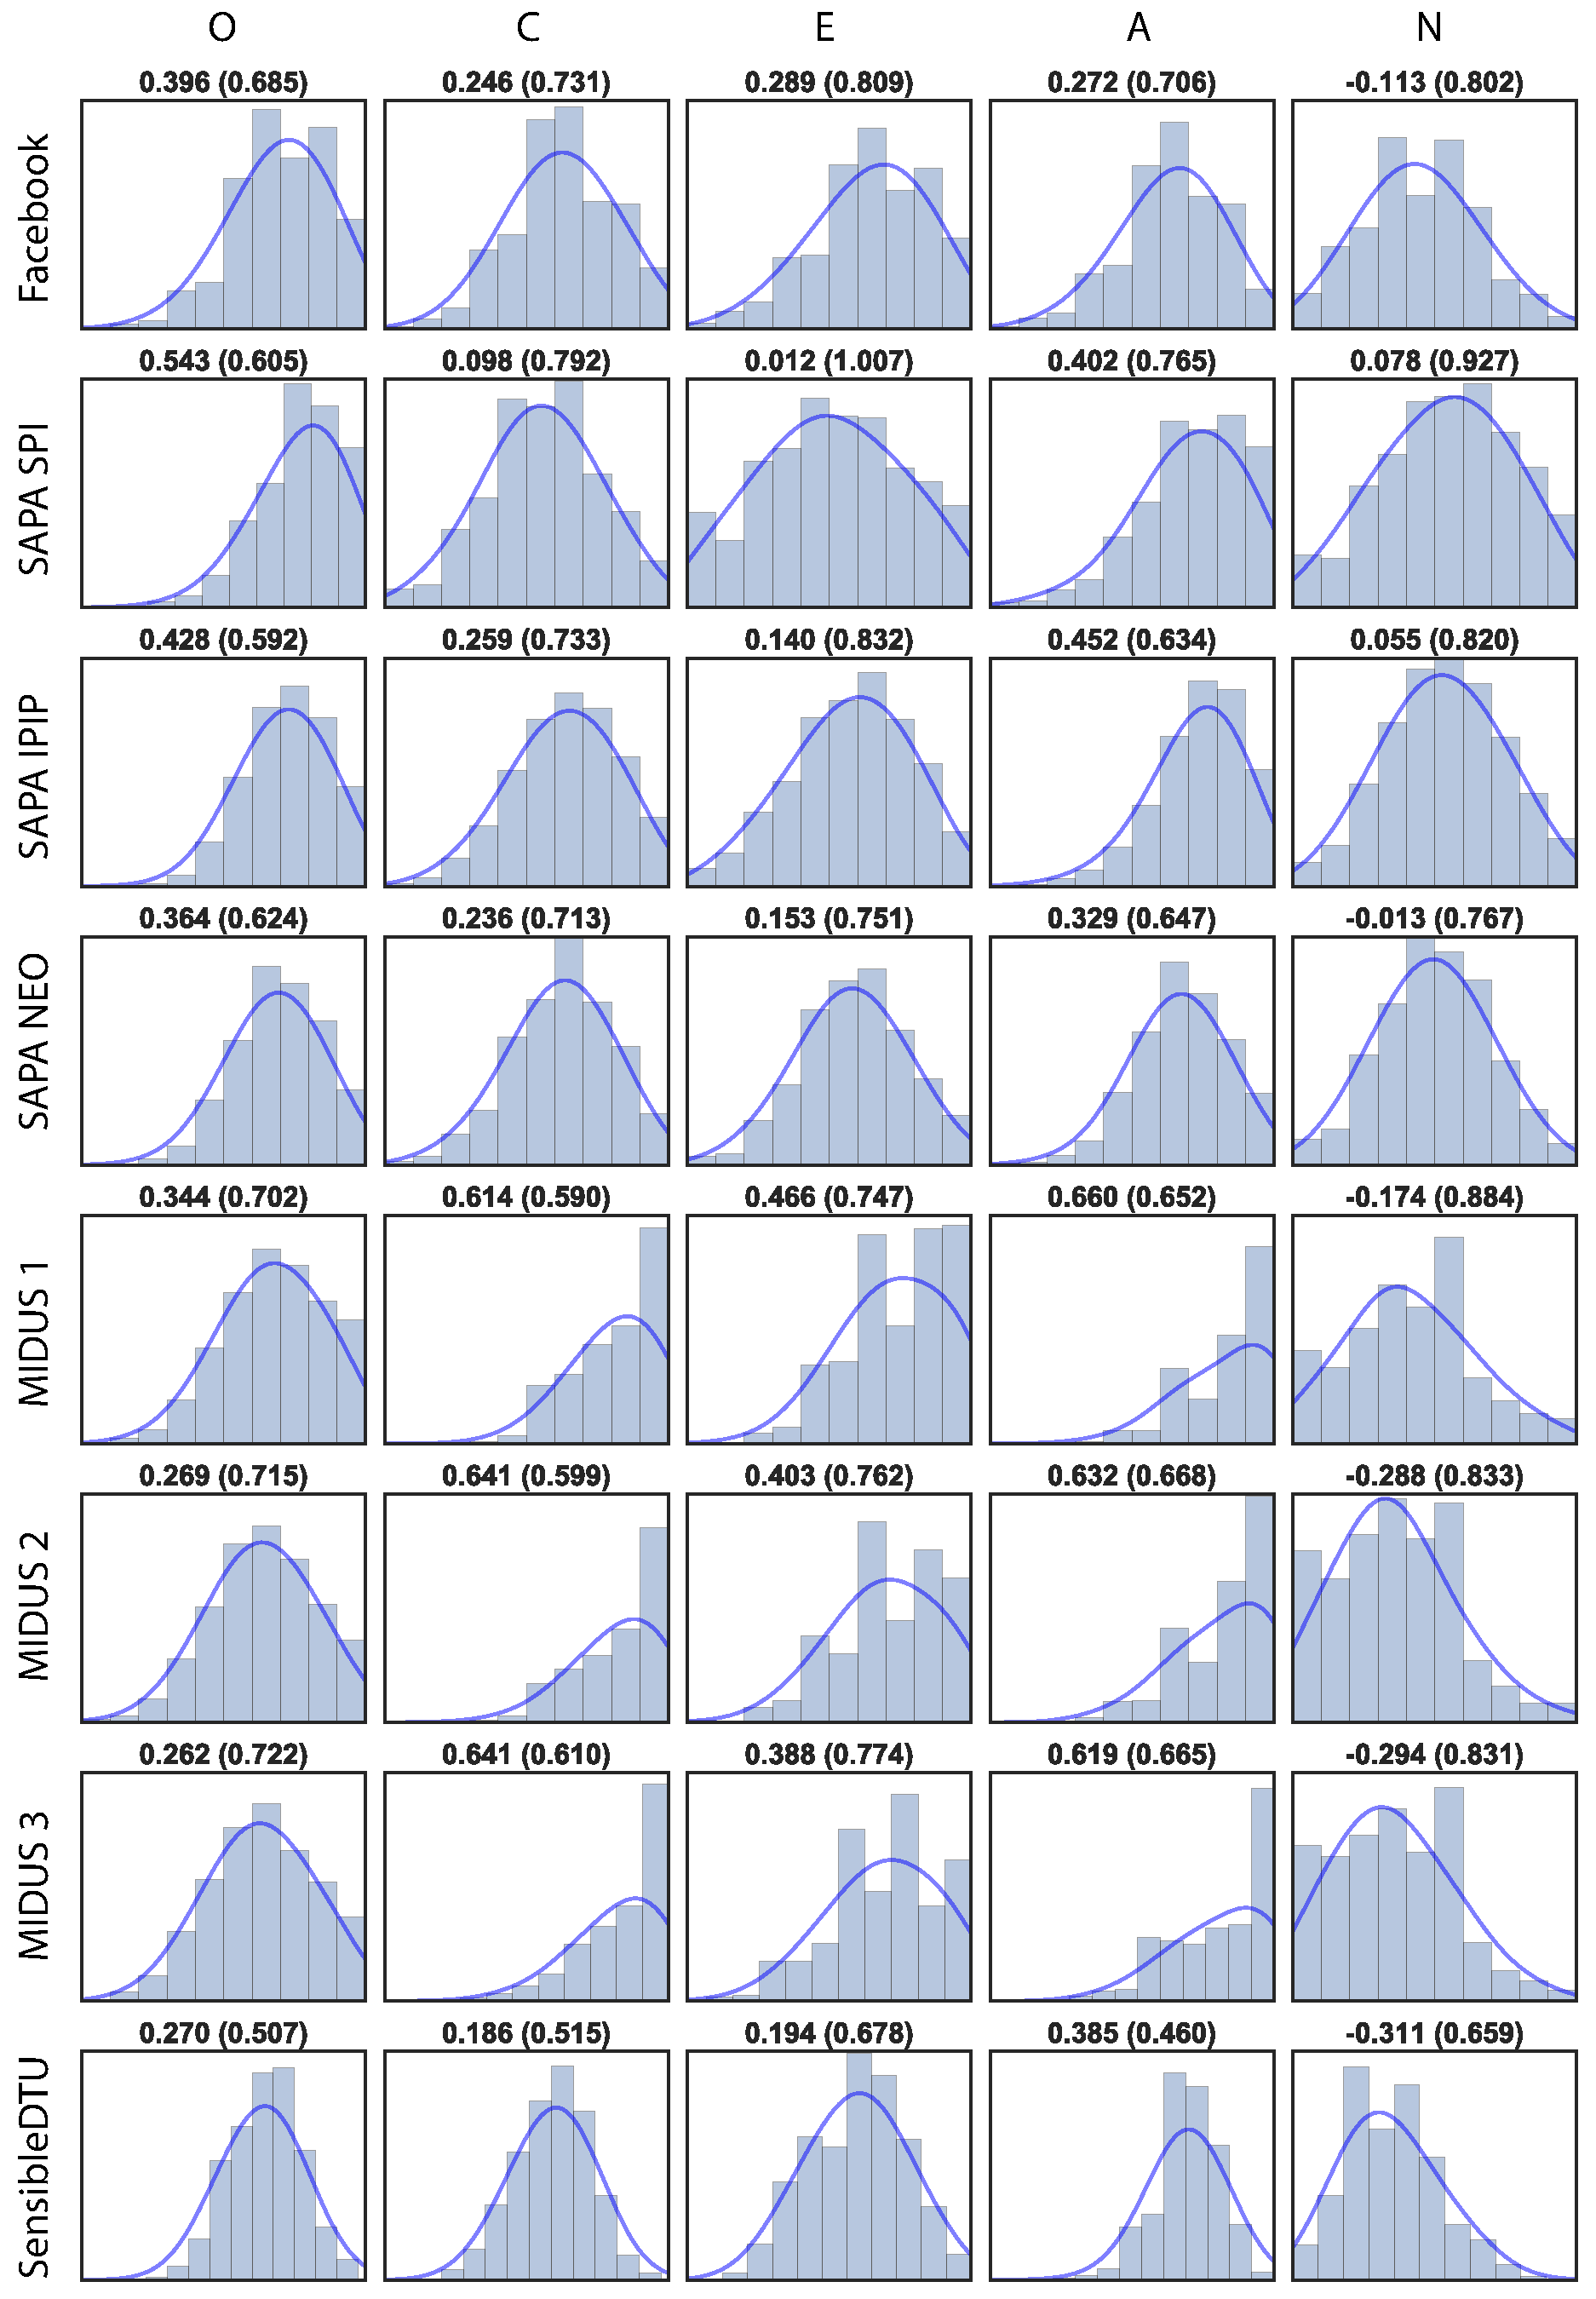
\includegraphics[width=\textwidth]{figures/dataDistributions}
\end{figure}
\newpage

% Code for enrichment of feautres near archetypes
\section{Code for enrichment of feautres near archetypes \label{app:enrichment_code}}
\thispagestyle{plain}
\begin{lstlisting}[language=Python, label={lst:enrichments}, caption="Python code for computing enrichments near archetypes"]
import numpy as np
from collections import Counter

def compute_a_c_bins(D, T):
    """Compute enrichment for features T using precomputed arc.-distances, D.

    Parameters
    ----------
    D : numpy.2darray (N, M)
        Precomputed distances between N points and M archetypes.
    T: pandas.DataFrame (N, K)
        K features for N individuals matching rows in D. Each
        feature (column) must have an associatec column label.

    Output
    ------
    a_c_bins : json-dict
        JSON data structure storing enrichments near each archetype for each
        feature.

        Example
        -------
        {'0': {
            'age': {
                        # 10 bin averages
                [34.1, 33.8, 33.2, 33.4, 32.5, 32.0, 32.2, 31.0, 30.9, 30.5],
                32.35,  # mean
                30.5,   # minimum
                34.1,   # maximum
                1.204,  # SD
                0.0231  # standard error
            }, 
            ...
            'job status', {
                [   
                    Counter({'employed': 42, ... , 'student': 12}),
                    ...
                    Counter({'employed': 12, ... , 'student': 42})
                ],  # 10 bin Counter dictionaries                               
                set(['employed', ..., 'student'])  # set of attributes
            }
        }}
    """
    a_c_bins = {}
    # Loop over arcs
    for a in range(D.shape[1]):
        Da = D[:, a]  # distances from arc
        c_bins = {}
        # Loop over enrichment features and build bins for each (b_bins)
        for c in df.columns:
            # Sort attributes into bins
            ca = np.vstack([df[c], Da]).T
            ca = ca[ca[:, 1].argsort()]
            ca = ca[np.array(map(lambda v: v==v, list(ca[:, 0]))), :]

            N = ca.shape[0]
            bins = []

            bin_intervals = zip(
                np.arange(0*N, 1*N, 0.1*N),
                np.arange(0.1*N, 1.1*N, 0.1*N)
            )

            # Continuous feature
            if type(ca[0, 0]) is not str:
                bins_std, bins_err = [], []
                for p_low, p_upp in bin_intervals:
                    bins.append(np.mean(ca[p_low:p_upp, 0]))
                    bins_std.append(np.std(ca[p_low:p_upp, 0]))
                    bins_err.append(
                        np.std(ca[p_low:p_upp, 0]) / np.sqrt(len(ca[p_low:p_upp, 0]))
                        )
                c_bins[c] = (
                    bins, np.mean(ca[:, 0]), np.min(ca[:, 0]),
                    np.max(ca[:, 0]), bins_std, bins_err
                )
            
            # Categorical feature
            else:
                attrs = set()
                for p_low, p_upp in bin_intervals:
                    counter = Counter(ca[p_low:p_upp, 0])
                    bins.append(counter)
                    attrs.update(counter.keys())
                c_bins[c] = (bins, list(attrs))

        a_c_bins[a] = c_bins
    return a_c_bins
\end{lstlisting}
\newpage

% Online
\section{Online \label{app:onlineAppendix1}}
\thispagestyle{plain}
$\,$\\

\vspace{-0.7cm}
\textbf{a)} Go to \url{ulfaslak.com/master_thesis/online_appendix1.pdf}.\\

% \textbf{b)} Go to \url{ulfaslak.com/master_thesis/online_appendix2.pdf}.\\

\newpage

\end{document}

